\documentclass[11pt]{article}
\usepackage{guide}
\reporttitle{C241 Test 1: The Study Guide I Wanted}{Jeryn Vicari}{Fall 2026}
\setcounter{tocdepth}{1}

\begin{document}
\makereporttitle

\begin{notebox}
\textbf{Unofficial.} This isn't from the course staff, and it doesn't replace the lecture notes. Where this guide and the notes disagree, the notes and your TA win. Every example and practice problem in here is new; none of it comes from the homework or quizzes.
\end{notebox}

\section*{How to use this}
\addcontentsline{toc}{section}{How to use this}

Test 1 covers sets, propositional logic, constrained proofs, relations up to symmetry, functions, and (probably) graphs. On paper that's six topics. In practice it's one idea used over and over: \emph{everything is a claim about membership}, and every claim is either ``for all'' or ``there exists.'' Once that clicks, the proof chapter stops feeling like a separate subject.

Each chapter goes the same way. First the intuition, in plain words. Then the precise definition, because the test grades the precise version. Then a picture, a worked example, and the places people usually slip. Every chapter ends with practice and full answers. The answers were checked by brute force on small examples, so you can trust them.

A few suggestions that are worth more than any single section:
\begin{itemize}
\item \textbf{Do the practice cold.} Read the chapter, close it, then try the problems with nothing open. If you can only do it with the notes next to you, you don't have it yet, and the test is closed-notes apart from one sheet.
\item \textbf{Write every column.} Most lost points on truth tables come from skipping an intermediate column, not from not knowing the connective.
\item \textbf{Proofs need reps, not reading.} Chapter 3 is the longest for a reason. Three short proofs a day for a week beats one long session the night before.
\item \textbf{Say ``member of'' and ``subset of.''} Never ``in.'' That one habit fixes half the set questions.
\end{itemize}

\begin{figure}[H]\centering
\begin{tikzpicture}[node distance=0.55cm and 0.9cm, every node/.style={font=\small}]
  \node[softbox,minimum width=3.1cm] (sets) {Ch 1: Sets\\ $\in$, $\subseteq$, $\cup\ \cap\ -$};
  \node[softbox,minimum width=3.1cm,right=of sets] (logic) {Ch 2: Logic\\ $\land\ \lor\ \lnot\ \to$, truth tables};
  \node[softbox,minimum width=3.1cm,right=of logic] (quant) {Ch 2: ``for all'' /\\ ``there exists''};
  \node[softbox,minimum width=5cm,below=1.1cm of logic,line width=1.2pt] (proofs) {Ch 3: Constrained proofs\\ 5 definitions + 7 rules};
  \node[softbox,minimum width=3.1cm,below=1.3cm of proofs,xshift=-4.4cm] (rel) {Ch 4: Relations\\ symmetry};
  \node[softbox,minimum width=3.1cm,below=1.3cm of proofs,xshift=0cm] (fun) {Ch 4: Functions\\ injective, onto};
  \node[softbox,minimum width=3.1cm,below=1.3cm of proofs,xshift=4.4cm] (gr) {Ch 5: Graphs\\ walks, paths, trees};
  \draw[->] (sets) -- (logic);
  \draw[->] (logic) -- (quant);
  \draw[->] (sets.south) |- ($(proofs.west)+(0,0.15)$);
  \draw[->] (logic) -- (proofs);
  \draw[->] (quant.south) |- ($(proofs.east)+(0,0.15)$);
  \draw[->] (proofs) -- (rel);
  \draw[->] (proofs) -- (fun);
  \draw[->] (proofs) -- (gr);
  \draw[->,dashed] (rel) -- node[lbl,above,font=\scriptsize] {special kind of} (fun);
  \draw[->,dashed] (rel.south) to[out=-25,in=-155] node[lbl,below] {edges are pairs too} (gr.south);
\end{tikzpicture}
\caption{How the chapters lean on each other. Proofs are the hub: symmetry, injectivity and ``is this a path'' are all claims you prove or refute with the same rules.}
\end{figure}

\tableofcontents
\clearpage

% Chapter 1: Sets (notes 1.1-1.5 and 2.5.1). Fragment: \input from the main file.
% Helper macros use the \sets prefix so they can't clash with other chapters.
\newcommand{\setsP}{\mathcal{P}}
\newcommand{\setsSt}{\mathrel{|}}
% \setsVenn{xshift}{fill commands}{label}: one two-circle Venn diagram inside a universe box
\newcommand{\setsVenn}[3]{%
  \begin{scope}[xshift=#1]
    \path[use as bounding box] (-0.2,-1.55) rectangle (2.5,1.1);
    #2
    \draw (-0.1,-0.95) rectangle (2.4,0.95);
    \node[font=\scriptsize,anchor=north west,inner sep=1.5pt] at (-0.1,0.95) {$\mathcal{U}$};
    \draw (0.8,0) circle (0.62);
    \draw (1.5,0) circle (0.62);
    \node[font=\scriptsize] at (0.45,0) {$A$};
    \node[font=\scriptsize] at (1.85,0) {$B$};
    \node[font=\small] at (1.15,-1.3) {#3};
  \end{scope}}

\section{Sets}

Almost everything in this course is built out of sets, and almost every set question on Test~1 comes down to one move: asking whether a specific thing is a member of a specific set. If you get good at that one move, the operations, subsets and power sets stop being separate topics. They're all membership questions in different clothes.

% ------------------------------------------------------------------
\subsection{Membership is the whole story}

Here's a set: $M=\{a,\ \{a\},\ \{b,c\}\}$. How many members does it have? Three. The letter $a$, the set $\{a\}$, and the set $\{b,c\}$. Is $b$ a member of $M$? No. The letter $b$ shows up on the page, but it's sitting inside one of $M$'s members, not in $M$'s own list.

That's the mindset for this whole chapter. A set is defined by which things are its members, and nothing else. There's no first member, no second member, no ``how many times'' a member appears. Something is either a member or it isn't.

\begin{notebox}
\textbf{Set, member.} A set is a thing that has members. $x\in A$ means ``$x$ is a member of $A$''; $x\notin A$ means it isn't. Two sets are the same set exactly when they have the same members.

\textbf{Set-list notation.} List the members between curly braces: $\{1,2,3\}$. Round parentheses or square brackets do \emph{not} make a set.

\textbf{Empty set.} The set with no members, written $\varnothing$ or $\{\}$.
\end{notebox}

Two consequences fall straight out of the definition. Order doesn't matter, so $\{3,1,2\}=\{1,2,3\}$. Repeats don't matter either, so $\{3,1,1,2\}=\{1,2,3\}$: writing $1$ twice just says ``$1$ is a member'' twice. When you write an answer in set-list notation, write each member once anyway. Repeats in an answer look like you think they count.

\textbf{Worked example.} With $M=\{a,\{a\},\{b,c\}\}$:
\begin{itemize}
  \item $a\in M$: yes, it's listed.
  \item $\{a\}\in M$: yes, also listed. So $M$ has both $a$ and $\{a\}$ as members, and they're different members.
  \item $\{b,c\}\in M$: yes.
  \item $b\in M$: no. It's a member of a member, which doesn't count.
  \item $\varnothing\in M$: no. Nothing in the list is the empty set.
\end{itemize}
For a set written in set-list form, membership is the dumbest possible check: is it literally one of the listed items? No other test applies.

\textbf{Where people slip.}
\begin{itemize}
  \item Reading ``$b$ appears somewhere inside the braces'' as ``$b\in M$''. Only the top-level items are members.
  \item Treating $\varnothing$ as a member of every set. It isn't (more on why people think so in \S\ref{sets:ein}).
  \item Writing $\epsilon$ for $\in$. In this course $\varepsilon$ means the empty string, so keep the symbols apart.
\end{itemize}

% ------------------------------------------------------------------
\subsection{Set-builder notation}

Listing members breaks down fast. You can't list the even integers, and ``$\{3,4,6,8,12,\dots\}$'' makes the reader guess the pattern. Set-builder notation gives a recipe instead: a template on the left of the bar, and the conditions the template's variables must meet on the right.

\begin{notebox}
\textbf{Set-builder notation.} $\{\text{template}\setsSt\text{condition}\}$ is the set of everything you can get by plugging values that meet the condition into the template, and nothing else. Read the bar as ``such that'' or ``where''.
\end{notebox}

So $\{3k+1\setsSt k\in\mathbb{N}\}=\{1,4,7,10,\dots\}$. To decide whether some $x$ is a member, you try to \emph{match} $x$ to the template with legal values. One successful match is enough, so a membership claim like this is really a ``there exists'' claim.

\textbf{Worked example.} Let $F=\{3k+1\setsSt k\in\mathbb{N}\}$.
\begin{itemize}
  \item $10\in F$? Set $3k+1=10$, so $k=3$, and $3\in\mathbb{N}$. Yes.
  \item $0\in F$? We'd need $3k+1=0$, so $k=-\tfrac13$, which isn't a natural number. No other $k$ works, so no.
  \item $-2\in F$? We'd need $k=-1\notin\mathbb{N}$. No. But change the condition to $k\in\mathbb{Z}$ and the answer flips to yes. The condition is part of the definition.
\end{itemize}

Sometimes nothing meets the condition. $\{x\in\mathbb{N}\setsSt x<0\}$ has no members, so it's just $\varnothing$ written in a roundabout way.

You'll also see the variable's home set written on the left, as in $\{x\in\mathbb{N}\setsSt x<0\}$. That means the same as $\{x\setsSt x\in\mathbb{N}\text{ and }x<0\}$.

\textbf{Where people slip.}
\begin{itemize}
  \item Finding one value that \emph{doesn't} match and concluding ``not a member''. You need to show that \emph{no} legal value matches.
  \item Forgetting the condition. Plugging $k=-1$ into $3k+1$ gives $-2$, but $-1$ isn't allowed when $k\in\mathbb{N}$.
\end{itemize}

% ------------------------------------------------------------------
\subsection{The number sets}

You'll use these constantly as universes and as conditions in set-builder notation.

\begin{center}
\begin{tabularx}{\linewidth}{@{}lL@{}}
\toprule
\textbf{Set} & \textbf{What's in it}\\
\midrule
$\mathbb{N}$ & natural numbers $\{0,1,2,3,\dots\}$. In this course $0\in\mathbb{N}$, no exceptions.\\
$\mathbb{Z}$ & integers $\{\dots,-2,-1,0,1,2,\dots\}$\\
$\mathbb{Q}$ & rationals: $\{\frac pq\setsSt p\in\mathbb{Z}\text{ and }q\in\mathbb{Z}\text{ and }q\neq0\}$\\
$\mathbb{R}$ & reals: anything on the number line, any decimal expansion\\
\bottomrule
\end{tabularx}
\end{center}

The $\mathbb{Q}$ definition is set-builder notation, so the rule from the last section applies: the question is whether a number \emph{can be written} as an integer over a nonzero integer, not how it happens to be written right now. $\frac{0.5}{0.25}$ doesn't look like it qualifies, but it equals $\frac21$, so it's rational. $\sqrt9=\frac31$ is rational. $\frac{\pi}{2}$ is a ratio, but not of integers, and it can't be rewritten as one, so it isn't.

\textbf{Where people slip.} Leaving $0$ out of $\mathbb{N}$ because an older book did. Also: $\mathbb{N}\subseteq\mathbb{Z}\subseteq\mathbb{Q}\subseteq\mathbb{R}$, so every integer is rational. ``Rational'' doesn't mean ``has a fraction bar''.

% ------------------------------------------------------------------
\subsection{Union, intersection, difference, complement}

You probably learned these as ``smush the lists together'' and ``keep the overlap''. That works for small listed sets, but it falls apart once sets are defined by conditions. The definitions you'll actually use in proofs are membership tests: each operation says exactly when some $x$ is a member of the result.

\begin{notebox}
\textbf{Union.} $x\in A\cup B$ means $x\in A$ or $x\in B$ (or both).\\
\textbf{Intersection.} $x\in A\cap B$ means $x\in A$ and $x\in B$.\\
\textbf{Relative complement (difference).} $x\in A-B$ means $x\in A$ and $x\notin B$.\\
\textbf{Complement.} $x\in\overline{A}$ means $x\notin A$. This only makes sense once a universe $\mathcal{U}$ is fixed; then $\overline{A}=\{x\in\mathcal{U}\setsSt x\notin A\}$.
\end{notebox}

Notice that each operation is a logic connective in disguise: $\cup$ is ``or'', $\cap$ is ``and'', $-$ is ``and not'', and the overline is ``not''. That link is why the logic in \S\ref{logic:start} keeps coming back to sets.

\begin{figure}[H]
\centering

\begin{tikzpicture}[shade/.style={fill=gray!35}]
  \setsVenn{0cm}{\fill[shade] (0.8,0) circle (0.62); \fill[shade] (1.5,0) circle (0.62);}{$A\cup B$}
  \setsVenn{3.05cm}{\begin{scope}\clip (0.8,0) circle (0.62); \fill[shade] (1.5,0) circle (0.62);\end{scope}}{$A\cap B$}
  \setsVenn{6.1cm}{\fill[shade] (0.8,0) circle (0.62); \fill[white] (1.5,0) circle (0.62);}{$A-B$}
  \setsVenn{9.15cm}{\fill[shade] (1.5,0) circle (0.62); \fill[white] (0.8,0) circle (0.62);}{$B-A$}
  \setsVenn{12.2cm}{\fill[shade] (-0.1,-0.95) rectangle (2.4,0.95); \fill[white] (0.8,0) circle (0.62);}{$\overline{A}$}
\end{tikzpicture}
\caption{The shaded region is everything that passes the membership test. $A-B$ and $B-A$ are different regions, and $\overline{A}$ fills the rest of the universe box, so it changes if the box changes.}
\end{figure}

\textbf{Worked example.} Take $\mathcal{U}=\{0,1,\dots,9\}$, $A=\{1,2,3,4\}$, $B=\{3,4,5,6\}$.
\begin{itemize}
  \item $A\cup B=\{1,2,3,4,5,6\}$.
  \item $A\cap B=\{3,4\}$.
  \item $A-B=\{1,2\}$. Go through $A$ member by member and drop anything in $B$.
  \item $B-A=\{5,6\}$. Different set. Difference isn't symmetric, the same way $7-3\neq3-7$.
  \item $\overline{A}=\{0,5,6,7,8,9\}$. Now shrink the universe to $\{1,\dots,6\}$ and $\overline{A}$ becomes $\{5,6\}$. Same $A$, different answer.
\end{itemize}

\textbf{Where people slip.}
\begin{itemize}
  \item Computing $B-A$ when asked for $A-B$. Always start from the \emph{left} set.
  \item Taking a complement without writing down the universe first. If a problem gives you $\overline{A}$, find the stated universe before doing anything else.
  \item Writing $A\land B$ when you mean $A\cap B$. Connectives join statements; $\cap$ and $\cup$ join sets. ``$x\in A\cap B$'' is fine, ``$x\in A\land B$'' is a type error.
\end{itemize}

% ------------------------------------------------------------------
\subsection{Cardinality}

\begin{notebox}
\textbf{Cardinality.} For a finite set $A$, $|A|$ is the number of members of $A$.
\end{notebox}

Count distinct members only, and count members, not symbols:
\begin{itemize}
  \item $|\{3,1,1,2\}|=3$, since the repeat collapses.
  \item $|\{\{1,2,3\}\}|=1$. One member, which happens to be a set with three members.
  \item $|\varnothing|=0$ and $|\{\varnothing,\{\varnothing\}\}|=2$.
  \item $|\{x\in\mathbb{Z}\setsSt 0<x^2<5\}|=4$, because the members are $-2,-1,1,2$.
\end{itemize}
For infinite sets like $\mathbb{Z}$, just say the set is infinite. Comparing sizes of infinite sets is a much later topic.

\textbf{Where people slip.} Counting the members of the members. In $\{\{1,2,3\}\}$ the inner $1,2,3$ are one level too deep to count.

% ------------------------------------------------------------------
\subsection{Subsets, proper subsets, set equality}

Membership relates a thing to a set. Subset relates a set to a set, and it's a statement about all of the first set's members at once.

\begin{notebox}
\textbf{Subset.} $A\subseteq B$ means every member of $A$ is a member of $B$. (Also written $B\supseteq A$, ``$B$ is a superset of $A$''.)\\
\textbf{Proper subset.} $A\subsetneq B$ means $A\subseteq B$ and $A\neq B$.\\
\textbf{Set equality.} $A=B$ exactly when $A\subseteq B$ and $B\subseteq A$.
\end{notebox}

The symbol $\subseteq$ looks like $\leq$ on purpose: every set is a subset of itself, the same way $5\leq5$. Avoid $\subset$ entirely. Some people read it as $\subseteq$ and others as $\subsetneq$.

Because ``every member'' is a universal claim, the two directions of proof are lopsided:
\begin{itemize}
  \item To show $A\subseteq B$, you have to cover \emph{every} member of $A$. For a short list, check them one by one. For a set-builder set, take an arbitrary member and argue it lands in $B$.
  \item To show $A\not\subseteq B$, you need \emph{one} member of $A$ that isn't in $B$. Name it.
\end{itemize}

\textbf{Worked example.}
\begin{itemize}
  \item $\{2,3\}\subseteq\{1,2,3\}$: both $2$ and $3$ are listed on the right. Since the sets differ, it's also $\{2,3\}\subsetneq\{1,2,3\}$.
  \item $\{0,5\}\not\subseteq\{n^2\setsSt n\in\mathbb{Z}\}$: the witness is $5$. It's in the left set, and $n^2=5$ has no integer solution.
  \item $\{n\in\mathbb{Z}\setsSt 0<n<4\}=\{1,2,3\}$. Left to right: an integer strictly between $0$ and $4$ is $1$, $2$ or $3$. Right to left: each of $1,2,3$ is an integer strictly between $0$ and $4$.
  \item $\{1,2\}$ and $\{2,3\}$: neither is a subset of the other ($1$ blocks one direction, $3$ the other). Unlike numbers, two sets don't have to be comparable.
\end{itemize}

One more structural fact: $\subseteq$ chains. If $A\subseteq B$ and $B\subseteq C$, then $A\subseteq C$. Membership does not chain: $1\in\{1\}$ and $\{1\}\in\{\{1\}\}$, but $1\notin\{\{1\}\}$, because the only member of $\{\{1\}\}$ is the set $\{1\}$.

\textbf{Where people slip.}
\begin{itemize}
  \item Proving $A\subseteq B$ by checking a couple of examples. That's evidence, not a proof, unless the examples are all of $A$'s members.
  \item Answering ``no'' to a subset question without naming the member that breaks it.
  \item Writing $\{1,2\}\subsetneq\{1,2\}$. Proper means the sets have to differ.
\end{itemize}

% ------------------------------------------------------------------
\subsection{\texorpdfstring{$\in$ versus $\subseteq$}{Member versus subset}}\label{sets:ein}

This is the single most common way to lose points on set questions, and the cause is a picture most people carry around: a set as a container, with stuff ``in'' it. The trouble is that ``in'' (and ``contains'') covers two different relationships. ``$\{1\}$ is in $\{1,2\}$'' could mean member or subset, and only one of those is true. So stop saying ``in'' and ``contains'' when you study. Say ``member of'' or ``subset of'', and the right answer usually becomes obvious.

\begin{figure}[H]
\centering
\begin{tikzpicture}[item/.style={draw,rectangle,inner sep=3pt,minimum height=1.5em,font=\small},
                    atom/.style={inner sep=2pt,font=\small}]
  % left panel: membership
  \begin{scope}
    \node[draw,rounded corners=3pt,minimum width=5.6cm,minimum height=2.3cm] (M1) at (0,0) {};
    \node[anchor=north west,font=\small] at (M1.north west) {$M$};
    \node[atom] (a1) at (-1.8,0.1) {$a$};
    \node[item] (A1) at (-0.3,0.1) {$a$};
    \node[item,hl] (BC1) at (1.5,0.1) {$b\quad c$};
    \node[font=\scriptsize] (bnote) at (1.5,-0.85) {$b$ is two levels down};
    \node[lbl,align=center] at (0,-1.75) {$\in$: point at \emph{one} item.\\ $\{b,c\}\in M$ \quad but \quad $b\notin M$};
  \end{scope}
  % right panel: subset
  \begin{scope}[xshift=7.4cm]
    \node[draw,rounded corners=3pt,minimum width=5.6cm,minimum height=2.3cm] (M2) at (0,0) {};
    \node[anchor=north west,font=\small] at (M2.north west) {$M$};
    \node[atom] (a2) at (-1.8,0.1) {$a$};
    \node[item] (A2) at (-0.3,0.1) {$a$};
    \node[item] (BC2) at (1.5,0.1) {$b\quad c$};
    \draw[dashed,rounded corners=6pt] ($(a2.south west)+(-0.25,-0.3)$) rectangle ($(A2.north east)+(0.25,0.3)$);
    \node[lbl,align=center] at (0,-1.75) {$\subseteq$: pick \emph{some} items, put them in a new box.\\ $\{a,\{a\}\}\subseteq M$};
  \end{scope}
\end{tikzpicture}
\caption{$M=\{a,\{a\},\{b,c\}\}$ drawn with a box for every pair of braces. Each inner box is a single item of $M$. A member is one item; a subset is a new box whose items all come from $M$'s items.}
\end{figure}

The working test for each:
\begin{itemize}
  \item ``$x\in Y$?'' Is $x$ one of $Y$'s items? Nothing else matters.
  \item ``$X\subseteq Y$?'' First, $X$ has to be a set. Then: is each item of $X$ one of $Y$'s items?
\end{itemize}

\textbf{Worked example.} Still with $M=\{a,\{a\},\{b,c\}\}$:
\begin{itemize}
  \item $\{a\}\in M$ and $\{a\}\subseteq M$. Both! It's listed, \emph{and} its only member $a$ is listed.
  \item $\{b,c\}\in M$, but $\{b,c\}\not\subseteq M$, because $b\notin M$.
  \item $\{b\}\notin M$ and $\{b\}\not\subseteq M$. Neither.
  \item $\varnothing\notin M$, but $\varnothing\subseteq M$.
\end{itemize}

That last pair is the classic. The empty set is a subset of every set: to break $\varnothing\subseteq M$ you'd need a member of $\varnothing$ that isn't in $M$, and $\varnothing$ has no members to offer. (That's vacuous truth, covered in the logic chapter.) But $\varnothing$ is a member of a set only if it's actually listed. The two facts get blurred into ``the empty set is in every set'', and that sentence is half wrong.

\textbf{Where people slip.}
\begin{itemize}
  \item Concluding $\{1,2,3\}\in\{0,1,2,3\}$ because ``all of its members are in there''. That argument proves $\subseteq$, never $\in$.
  \item Writing $2\subseteq\{1,2\}$. A number isn't a set, so it can't be a subset of anything. Write $\{2\}\subseteq\{1,2\}$ or $2\in\{1,2\}$.
\end{itemize}

% ------------------------------------------------------------------
\subsection{\texorpdfstring{Wrapping in braces: $1$ vs $\{1\}$, $\varnothing$ vs $\{\varnothing\}$}{Wrapping in braces}}

Every pair of braces makes a new object. $\{1\}$ is not a fancier way to write $1$; it's a set whose one member is the number $1$. Same for $\varnothing$ and $\{\varnothing\}$: the first is an empty box, the second is a box with one item, and that item happens to be an empty box.

\begin{figure}[H]
\centering
\begin{tikzpicture}[set/.style={draw,rectangle,inner sep=4pt,minimum height=1.6em,minimum width=1.6em,font=\small}]
  \node[font=\small] (n1) at (0,0) {$1$};
  \node[set] (s1) at (2.0,0) {$1$};
  \node[set] (e0) at (4.4,0) {};
  \node[set,minimum width=2.4em,minimum height=2.4em] (e1) at (6.6,0) {};
  \node[set,minimum width=0.9em,minimum height=0.9em,inner sep=0pt] at (e1) {};
  \node[set,minimum width=5.0em,minimum height=2.4em] (e2) at (9.6,0) {};
  \node[set,minimum width=0.9em,minimum height=0.9em,inner sep=0pt] at ($(e2)+(-0.45,0)$) {};
  \node[set,minimum width=1.6em,minimum height=1.6em,inner sep=0pt] (inner) at ($(e2)+(0.45,0)$) {};
  \node[set,minimum width=0.6em,minimum height=0.6em,inner sep=0pt] at (inner) {};
  \foreach \n/\t/\c in {n1/{$1$}/{a number},s1/{$\{1\}$}/{1 member},e0/{$\varnothing$}/{0 members},e1/{$\{\varnothing\}$}/{1 member},e2/{$\{\varnothing,\{\varnothing\}\}$}/{2 members}}
    \node[font=\small,align=center] at ($(\n)+(0,-1.0)$) {\t\\[-1pt]\footnotesize\c};
\end{tikzpicture}
\caption{Each box is one pair of braces. Count a set's members by counting the items directly inside its outer box.}
\end{figure}

Facts worth having cold:
\begin{itemize}
  \item $1\neq\{1\}$. One is a number, the other a set.
  \item $1\in\{1\}$, $\{1\}\in\{\{1\}\}$, but $1\notin\{\{1\}\}$.
  \item $\{1\}\subseteq\{1,2\}$ but $\{1\}\notin\{1,2\}$.
  \item $|\varnothing|=0$ but $|\{\varnothing\}|=1$. So $\{\varnothing\}\neq\varnothing$.
  \item $\varnothing\in\{\varnothing\}$ and $\varnothing\subseteq\{\varnothing\}$. Both, for different reasons.
\end{itemize}

\textbf{Where people slip.} Writing an answer like $A\cap B=3$ when the answer is the set $\{3\}$. An operation on sets always gives a set, even when it has one member.

% ------------------------------------------------------------------
\subsection{Power sets}

\begin{notebox}
\textbf{Power set.} $\setsP(A)=\{B\setsSt B\subseteq A\}$, the set of all subsets of $A$.\\
For finite $A$, $|\setsP(A)|=2^{|A|}$.
\end{notebox}

Read the definition as a membership test, because that's how you'll use it: $X\in\setsP(A)$ means exactly $X\subseteq A$. Every question of the form ``is this in the power set?'' turns into a subset question.

To list $\setsP(A)$ without missing anything, go by size: the empty set, then all one-member subsets, then all two-member subsets, and so on up to $A$ itself.

\begin{figure}[H]
\centering
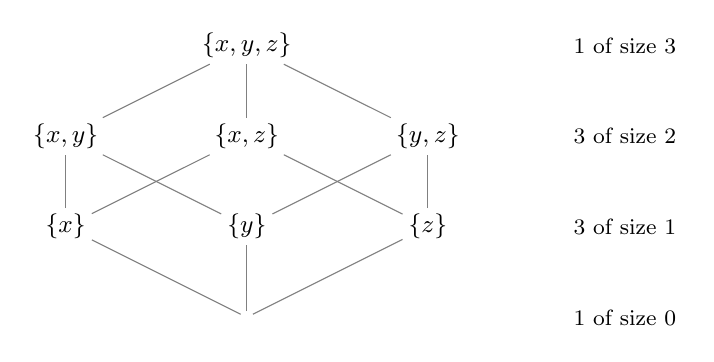
\begin{tikzpicture}[ps/.style={inner sep=2pt,font=\small},x=2.3cm,y=1.15cm]
  \node[ps] (e)   at (0,0)  {$\varnothing$};
  \node[ps] (x)   at (-1,1) {$\{x\}$};
  \node[ps] (y)   at (0,1)  {$\{y\}$};
  \node[ps] (z)   at (1,1)  {$\{z\}$};
  \node[ps] (xy)  at (-1,2) {$\{x,y\}$};
  \node[ps] (xz)  at (0,2)  {$\{x,z\}$};
  \node[ps] (yz)  at (1,2)  {$\{y,z\}$};
  \node[ps] (xyz) at (0,3)  {$\{x,y,z\}$};
  \foreach \a/\b in {e/x,e/y,e/z,x/xy,x/xz,y/xy,y/yz,z/xz,z/yz,xy/xyz,xz/xyz,yz/xyz}
    \draw[gray] (\a) -- (\b);
  \foreach \yy/\c in {0/1,1/3,2/3,3/1}
    \node[font=\footnotesize,anchor=west] at (1.75,\yy) {\c\ of size \yy};
\end{tikzpicture}
\caption{All eight members of $\setsP(\{x,y,z\})$. A line joins two subsets when the upper one adds exactly one member. Row counts $1+3+3+1=8=2^3$.}
\end{figure}

Why $2^{|A|}$? Building a subset means making one yes/no decision per member of $A$: in or out. Three members, three independent binary choices, $2\cdot2\cdot2=8$ subsets. It's the same count as the rows of a truth table with three variables, and that's not a coincidence.

\textbf{Worked example.}
\begin{itemize}
  \item $\setsP(\{x,y,z\})=\{\varnothing,\{x\},\{y\},\{z\},\{x,y\},\{x,z\},\{y,z\},\{x,y,z\}\}$. Both $\varnothing$ and the whole set are always in there.
  \item $\setsP(\varnothing)=\{\varnothing\}$. The empty set has exactly one subset (itself), so $|\setsP(\varnothing)|=1=2^0$.
  \item $|\setsP(\setsP(\{1\}))|$: $\setsP(\{1\})=\{\varnothing,\{1\}\}$ has 2 members, so the answer is $2^2=4$.
\end{itemize}

\textbf{Where people slip.}
\begin{itemize}
  \item Writing $1\in\setsP(\{1,2\})$. Members of a power set are \emph{sets}. The member is $\{1\}$.
  \item Claiming $A\subseteq\setsP(A)$. Usually false: the members of $A$ are things like numbers, the members of $\setsP(A)$ are sets. What's true is $A\in\setsP(A)$.
  \item Forgetting $\varnothing$ or $A$ itself when listing, then getting $2^n-1$ or $2^n-2$.
\end{itemize}

% ------------------------------------------------------------------
\subsection{Practice}

None of these come from homework. Try each one cold before you look at the answers; the point is to find out what you can do with nothing in front of you.

\begin{enumerate}[label=\textbf{\arabic*.},leftmargin=1.8em,itemsep=0.35em]
  \item Let $P=\{2,\{2\},\{2,3\},\varnothing\}$. For each $x$ below, say whether $x\in P$, whether $x\subseteq P$, both, or neither:\\
  (a) $\varnothing$ \quad (b) $\{2\}$ \quad (c) $2$ \quad (d) $\{2,3\}$ \quad (e) $\{\{2\}\}$ \quad (f) $\{3\}$
  \item Universe $\mathcal{U}=\{0,1,\dots,11\}$. Let $E=\{n\in\mathcal{U}\setsSt n\text{ is even}\}$ and $T=\{3k\setsSt k\in\mathbb{N}\text{ and }3k\leq 11\}$. Write in set-list notation: $E\cap T$, $T-E$, $E-T$, $\overline{E\cup T}$. Then compute $\overline{E}\cap\overline{T}$ and compare it with $\overline{E\cup T}$.
  \item Let $W=\{k^2+1\setsSt k\in\mathbb{Z}\}$. Which of $10, 1, 3, 0, 26$ are members of $W$? Then let $H=\{\frac ab\setsSt a\in\mathbb{N}\text{ and }b\in\mathbb{N}\text{ and }b\neq0\}$. Is $0\in H$? Is $0.75\in H$? Is $-\frac23\in H$?
  \item Write $\{x\in\mathbb{Z}\setsSt x^2<10\}$ in set-list notation and give its cardinality. Do the same with $\mathbb{N}$ in place of $\mathbb{Z}$.
  \item Let $Y=\{a,\{b\}\}$. List $\setsP(Y)$. What is $|\setsP(\setsP(Y))|$? Is $\{b\}\in\setsP(Y)$? Is $\{\{b\}\}\in\setsP(Y)$?
  \item True or false, with a one-line reason each:\\
  (a) $\varnothing\subseteq\varnothing$ \quad (b) $\varnothing\in\varnothing$ \quad (c) $\varnothing\in\{\varnothing\}$\\ (d) $\{\varnothing\}\subseteq\varnothing$ \quad (e) $|\{\varnothing,\{\varnothing\}\}|=2$ \quad (f) $\setsP(\varnothing)=\varnothing$
  \item (a) Find a nonempty set $A$ and a set $B$ with both $A\in B$ and $A\subseteq B$.\\
  (b) Find a set $x$ with both $x\in\{x\}$ and $x\subseteq\{x\}$.
  \item Let $A=\{1,2,3\}$ and $B=\{3,4\}$. Each statement has one mistake. Find it and fix it.\\
  (a) ``$\{3\}\in A$, because $3\in A$.'' \quad (b) ``$A-B=\{4\}$.'' \quad (c) ``$A\cap B=3$.''\\
  (d) ``$\varnothing\in A$, because the empty set is in every set.'' \quad (e) ``$\{1,2,3,3\}$ has four members.''
  \item (a) How many subsets of $\{1,2,3,4,5\}$ have $1$ as a member but not $2$?\\
  (b) How many proper subsets does $\{1,2,3,4,5\}$ have?
\\  (c) What is $|\setsP(\{1,2\})\cup\{1,2\}|$?
  \item Let $X=\{1,2\}$. True or false:\\ (a) $X\in\setsP(X)$ \quad (b) $X\subseteq\setsP(X)$ \quad (c) $\{X\}\subseteq\setsP(X)$\\ (d) $\setsP(X)\cap X=\varnothing$ \quad (e) $\varnothing\in\setsP(X)\cap X$
  \item True or false, with justification:\\
  (a) $\{n\in\mathbb{Z}\setsSt n^2=n\}=\{0,1\}$ \quad
  (b) $\{3n+1\setsSt n\in\mathbb{Z}\}=\{3n-2\setsSt n\in\mathbb{Z}\}$\\
  (c) $\{n^2\setsSt n\in\mathbb{N}\}\subsetneq\mathbb{N}$ \quad
  (d) $\{3n+1\setsSt n\in\mathbb{N}\}=\{3n-2\setsSt n\in\mathbb{N}\}$
\end{enumerate}

% ------------------------------------------------------------------
\subsection{Answers}

Every answer here was checked by brute force.

\begin{enumerate}[label=\textbf{\arabic*.},leftmargin=1.8em,itemsep=0.45em]
  \item The members of $P$ are exactly the four listed items: $2$, $\{2\}$, $\{2,3\}$, $\varnothing$.
  \begin{itemize}
    \item (a) $\varnothing$: both. It's listed, and it's a subset of everything.
    \item (b) $\{2\}$: both. It's listed, and its one member $2$ is also listed.
    \item (c) $2$: member only. The subset question doesn't even apply, because $2$ isn't a set.
    \item (d) $\{2,3\}$: member only. It's listed, but $3\notin P$, so it isn't a subset.
    \item (e) $\{\{2\}\}$: subset only. Its one member $\{2\}$ is listed, but $\{\{2\}\}$ itself isn't.
    \item (f) $\{3\}$: neither. Not listed, and $3\notin P$.
  \end{itemize}
  \item First list the sets: $E=\{0,2,4,6,8,10\}$, $T=\{0,3,6,9\}$ (note $k=0$ gives $0$, since $0\in\mathbb{N}$).
  $E\cap T=\{0,6\}$. $T-E=\{3,9\}$. $E-T=\{2,4,8,10\}$. $E\cup T=\{0,2,3,4,6,8,9,10\}$, so $\overline{E\cup T}=\{1,5,7,11\}$.
  $\overline{E}=\{1,3,5,7,9,11\}$ and $\overline{T}=\{1,2,4,5,7,8,10,11\}$, so $\overline{E}\cap\overline{T}=\{1,5,7,11\}$. Same set. That makes sense: ``not in $E$ and not in $T$'' says the same thing as ``not in either''.
  \item $W$: $10=3^2+1$, yes. $1=0^2+1$, yes. $3$ would need $k^2=2$, no integer works, so no. $0$ would need $k^2=-1$, no. $26=5^2+1$, yes.
  $H$: $0=\frac01$ with $0\in\mathbb{N}$ and $1\neq0$, so yes. $0.75=\frac34$, yes. $-\frac23$: no. Both $a$ and $b$ are natural numbers, so every $\frac ab$ is $\geq0$, and no rewriting can make it negative.
  \item The integers with $x^2<10$ are $-3,\dots,3$ (since $4^2=16$). So $\{-3,-2,-1,0,1,2,3\}$, cardinality $7$. With $\mathbb{N}$: $\{0,1,2,3\}$, cardinality $4$.
  \item $\setsP(Y)=\{\varnothing,\{a\},\{\{b\}\},\{a,\{b\}\}\}$. That's $2^2=4$ members, so $|\setsP(\setsP(Y))|=2^4=16$.
  $\{b\}\in\setsP(Y)$ would mean $\{b\}\subseteq Y$, i.e.\ $b\in Y$. But $Y$'s members are $a$ and $\{b\}$, not $b$. So no.
  $\{\{b\}\}\in\setsP(Y)$ means $\{\{b\}\}\subseteq Y$, i.e.\ $\{b\}\in Y$, which is true. Yes.
  \item (a) True: $\varnothing$ is a subset of every set, itself included. (b) False: $\varnothing$ has no members at all. (c) True: it's the one listed member. (d) False: $\varnothing$ is a member of $\{\varnothing\}$ but not of $\varnothing$. (e) True: two distinct listed members. (f) False: $\setsP(\varnothing)=\{\varnothing\}$, which has one member.
  \item (a) One choice: $A=\{1\}$, $B=\{1,\{1\}\}$. $A$ is listed in $B$, so $A\in B$; and $A$'s only member $1$ is listed in $B$, so $A\subseteq B$. (b) $x=\varnothing$. $\varnothing\in\{\varnothing\}$ because it's listed, and $\varnothing\subseteq\{\varnothing\}$ because $\varnothing$ is a subset of everything.
  \item (a) $3\in A$ shows $\{3\}\subseteq A$, not $\{3\}\in A$. $A$'s members are numbers, so no set is a member of $A$.
  (b) $\{4\}$ is $B-A$. Start from $A$: $A-B=\{1,2\}$.
  (c) The intersection is a set: $A\cap B=\{3\}$.
  (d) $\varnothing\subseteq A$ is true, but $\varnothing\notin A$, since it isn't listed.
  (e) Repeats don't count. It has three members.
  \item (a) $1$ is forced in and $2$ is forced out. Each of $3,4,5$ is a free in/out choice: $2^3=8$.
  (b) $2^5=32$ subsets in all, minus the set itself: $31$.
  (c) $\setsP(\{1,2\})$ has four members, all sets: $\varnothing,\{1\},\{2\},\{1,2\}$. The numbers $1$ and $2$ are not among them, so the union has $4+2=6$ members.
  \item (a) True: $X\subseteq X$. (b) False: $1\in X$ but $1\notin\setsP(X)$ (only sets are members of $\setsP(X)$). (c) True: the one member of $\{X\}$ is $X$, and $X\in\setsP(X)$. (d) True: $X$'s members are numbers and $\setsP(X)$'s are sets, so they share nothing. (e) False: by (d), $\setsP(X)\cap X$ is $\varnothing$, which has no members.
  \item (a) True. $n^2=n$ means $n(n-1)=0$, so $n=0$ or $n=1$, and both are integers. Both directions of $\subseteq$ hold.
  (b) True. Every $3n+1$ equals $3(n+1)-2$ with $n+1\in\mathbb{Z}$, so left $\subseteq$ right. Every $3n-2$ equals $3(n-1)+1$ with $n-1\in\mathbb{Z}$, so right $\subseteq$ left. Same set, written two ways.
  (c) True. Every $n^2$ with $n\in\mathbb{N}$ is a natural number, so $\subseteq$ holds. And $2\in\mathbb{N}$ isn't a perfect square, so the sets differ.
  (d) False. $-2=3\cdot0-2$ is a member of the right set, but every member of the left set is at least $1$. The shift trick from (b) needs $n-1\in\mathbb{N}$, which fails at $n=0$.
\end{enumerate}

\clearpage
% Chapter 2: Propositional logic and claims (notes 2.1-2.5.2). Fragment: \input from the main file.
% Helper macros use the \log prefix so they can't clash with other chapters.
% \logCell{col}{row}{T or F}: one cell of a 2x2 assignment grid, shaded when the value is T
\newcommand{\logCell}[3]{%
  \if T#3\fill[gray!35] (#1*0.62,-#2*0.62) rectangle ++(0.62,-0.62);\fi
  \node[font=\scriptsize] at (#1*0.62+0.31,-#2*0.62-0.31) {#3};}
% \logGrid{xshift}{title}{TT}{TF}{FT}{FF}: satisfying assignments of a two-variable connective
\newcommand{\logGrid}[6]{%
  \begin{scope}[xshift=#1]
    \logCell{0}{0}{#3}\logCell{1}{0}{#4}\logCell{0}{1}{#5}\logCell{1}{1}{#6}
    \draw[step=0.62] (0,-1.24) grid (1.24,0);
    \node[font=\scriptsize] at (0.31,0.2) {$\mathrm{T}$};
    \node[font=\scriptsize] at (0.93,0.2) {$\mathrm{F}$};
    \node[font=\scriptsize] at (-0.22,-0.31) {$\mathrm{T}$};
    \node[font=\scriptsize] at (-0.22,-0.93) {$\mathrm{F}$};
    \node[font=\scriptsize] at (-0.3,0.25) {$P\backslash Q$};
    \node[font=\small] at (0.62,-1.62) {#2};
  \end{scope}}
\newcommand{\logT}{\mathrm{T}}
\newcommand{\logF}{\mathrm{F}}

\section{Propositional logic and claims}\label{logic:start}

The ideas in this chapter aren't hard. What costs points is \emph{evidence}, because the course is strict about it: a truth table with a skipped column, ``tautology'' with no table, ``not equivalent'' without naming the assignment that shows it. So along with the ideas, this chapter keeps saying exactly what you have to write down to back each one up.

% ------------------------------------------------------------------
\subsection{Propositions and expressions}

Compare ``$A\cap B$'' with ``$A\cap B=\varnothing$''. The first one names a thing (a set). The second one says something about that thing, and it's either true or false. That's the whole distinction.

\begin{notebox}
\textbf{Proposition.} A statement: something that asserts a fact and so is true or false (even if you don't know which yet, or it depends on a variable).\\
\textbf{Expression.} Something that names a value: a number, a set, a string. ``$x^2-3$'', ``$A\cup B$'', ``the set of odd primes''.
\end{notebox}

``$n^2+1$ is prime'' is a proposition, even though whether it's true depends on $n$. Questions (``Is 7 prime?''), commands (``Close the door.'') and bare noun phrases aren't propositions.

An \emph{atomic} proposition can't be split into smaller propositions. A \emph{compound} one is built from smaller ones with connectives. We use capital letters $P,Q,R$ for atomic propositions and lowercase $p,q$ for any formula.

\textbf{Where people slip.} Treating an expression as a statement. ``Assume $A\cap B$'' is nonsense, because you can't assume a set. You can assume $x\in A\cap B$.

% ------------------------------------------------------------------
\subsection{Connectives and truth tables}

There are six connectives. Each one is defined by its truth table: one row per combination of truth values for its parts.

\begin{center}
\begin{tabular}{cc|c|ccccc}
\toprule
$P$ & $Q$ & $\lnot P$ & $P\land Q$ & $P\lor Q$ & $P\oplus Q$ & $P\to Q$ & $P\leftrightarrow Q$\\
\midrule
T & T & F & T & T & F & T & T\\
T & F & F & F & T & T & F & F\\
F & T & T & F & T & T & T & F\\
F & F & T & F & F & F & T & T\\
\bottomrule
\end{tabular}
\end{center}

Names: $\land$ conjunction (``and''), $\lor$ inclusive disjunction (``or'', and both is fine), $\oplus$ exclusive disjunction (exactly one), $\lnot$ negation, $\to$ conditional (``if \dots\ then''), $\leftrightarrow$ biconditional (``if and only if'').

\begin{figure}[htb]
\centering
\begin{tikzpicture}
  \logGrid{0cm}{$P\land Q$}{T}{F}{F}{F}
  \logGrid{3.1cm}{$P\lor Q$}{T}{T}{T}{F}
  \logGrid{6.2cm}{$P\oplus Q$}{F}{T}{T}{F}
  \logGrid{9.3cm}{$P\to Q$}{T}{F}{T}{T}
  \logGrid{12.4cm}{$P\leftrightarrow Q$}{T}{F}{F}{T}
\end{tikzpicture}
\caption{The same tables as pictures. Each grid has one cell per truth assignment; shaded cells are the ones that satisfy the formula. $P\to Q$ has exactly one unshaded cell.}
\end{figure}

The one that trips people is $\to$. The way to remember it: a conditional is a promise, and the only way to break ``if $P$ then $Q$'' is to have $P$ happen and $Q$ not happen. That's the $(\logT,\logF)$ row. When $P$ is false, the promise was never tested, so the conditional counts as true. A few names you'll need: in $P\to Q$, $P$ is the \emph{premise} and $Q$ is the \emph{conclusion}.

\textbf{Where people slip.}
\begin{itemize}
  \item Making the bottom two rows of $P\to Q$ false. A false premise makes the whole conditional true.
  \item Using $\oplus$ for an ordinary ``or''. Inclusive is the default. Use $\oplus$ only for ``but not both'', ``exactly one of'', or very strong context.
  \item Writing $A\to B\to C$. Arrow isn't associative, so you must parenthesize. ($A\land B\land C$ is fine.)
  \item Mixing up the math symbols with code. In C, \texttt{\^{}} is exclusive or ($\oplus$), and there's no arrow at all.
\end{itemize}

% ------------------------------------------------------------------
\subsection{Translating English}

Translation goes in two steps. First, define atomic propositions, as small as you can, and keep the negation out of them (``$S$: the server is up'', not ``$S$: the server is down''). Then find the connective words and decide which chunk is a premise and which is a conclusion.

\begin{center}
\begin{tabularx}{\linewidth}{@{}Lc@{}}
\toprule
\textbf{English} & \textbf{Logic}\\
\midrule
$P$ and $Q$; $P$ but $Q$; $P$, yet $Q$; $P$, however $Q$ & $P\land Q$\\
$P$ or $Q$ (default); $P$ and/or $Q$; at least one of $P,Q$ & $P\lor Q$\\
exactly one of $P,Q$; $P$ or $Q$ but not both & $P\oplus Q$\\
neither $P$ nor $Q$ & $\lnot P\land\lnot Q$\\
$P$ unless $Q$ & $P\lor Q$\\
if $P$ then $Q$; $Q$ if $P$; $Q$ whenever $P$; $Q$ provided that $P$ & $P\to Q$\\
$P$ only if $Q$ & $P\to Q$\\
$P$ is sufficient for $Q$ & $P\to Q$\\
$P$ is necessary for $Q$ & $Q\to P$\\
$P$ if and only if $Q$; $P$ is necessary and sufficient for $Q$ & $P\leftrightarrow Q$\\
\bottomrule
\end{tabularx}
\end{center}

A few of these deserve a reason, so you can rebuild them under pressure:
\begin{itemize}
  \item \textbf{``But''} has the same truth table as ``and''. The contrast it adds is tone, not logic.
  \item \textbf{``Unless''} is an ``or'' word. ``We'll be there unless the car breaks down'' is false only if we aren't there \emph{and} the car didn't break down. That's the one $\logF$ row of $\lor$. (Context can push it to exclusive, but inclusive is the default.)
  \item \textbf{``If''} marks the premise wherever it appears in the sentence. So do ``whenever'', ``provided that'', ``in case'', ``given that''.
  \item \textbf{``Only if''} flips that: ``only'' plus a premise word marks the \emph{conclusion}. ``You can board only if you have a ticket'' means boarding $\to$ ticket. It does not promise that a ticket gets you on.
  \item \textbf{Sufficient} goes in the premise slot; \textbf{necessary} goes in the conclusion slot. Something necessary for $C$ is something $C$ can't happen without, so $C\to N$.
\end{itemize}

\textbf{Worked example.} Atoms: $S$ = ``the server is up'', $B$ = ``the backup ran'', $A$ = ``an alert fires''.
\begin{itemize}
  \item ``The server is up, but the backup didn't run.'' \quad $S\land\lnot B$
  \item ``An alert fires unless the backup ran.'' \quad $A\lor B$
  \item ``The backup runs only if the server is up.'' \quad $B\to S$
  \item ``The server being up is necessary for the backup to run.'' \quad $B\to S$ (the same claim as the last one)
  \item ``The backup running is sufficient for no alert.'' \quad $B\to\lnot A$
  \item ``Neither is the server up nor did the backup run.'' \quad $\lnot S\land\lnot B$
  \item ``An alert fires if and only if the server is down.'' \quad $A\leftrightarrow\lnot S$
\end{itemize}

\textbf{Where people slip.}
\begin{itemize}
  \item Translating ``$P$ only if $Q$'' as $Q\to P$. Read ``only if'' as ``then''.
  \item Putting the necessary condition in the premise.
  \item Reading an arrow as cause and effect. ``If there's smoke, there's fire'' is $\textit{smoke}\to\textit{fire}$, even though the fire causes the smoke. A conditional only says which combinations are allowed.
\end{itemize}

% ------------------------------------------------------------------
\subsection{Truth assignments and satisfaction}

A formula like $P\to Q$ isn't true or false on its own, any more than $x+y\leq5$ is. You need values for the variables first.

\begin{notebox}
\textbf{Truth assignment.} A choice of $\logT$ or $\logF$ for each atomic variable, e.g.\ $(P{=}\logT,Q{=}\logF)$.\\
\textbf{Satisfies.} An assignment satisfies a formula when the formula comes out $\logT$ under it.\\
\textbf{Satisfiable:} at least one assignment satisfies it.\quad
\textbf{Tautology:} every assignment satisfies it.\\
\textbf{Contradiction:} no assignment satisfies it.\quad
\textbf{Contingency:} at least one assignment satisfies it and at least one doesn't.
\end{notebox}

Say ``truth assignment'' and ``satisfying assignment'', never ``true assignment''. A truth table is just a tidy list of every assignment, one per row. With $n$ variables there are $2^n$ rows (same count as $|\mathcal{P}(A)|$ with $|A|=n$, because each variable is an independent in/out choice).

Every formula is exactly one of tautology, contingency, contradiction. Satisfiable means ``tautology or contingency''.

\begin{figure}[htb]
\centering
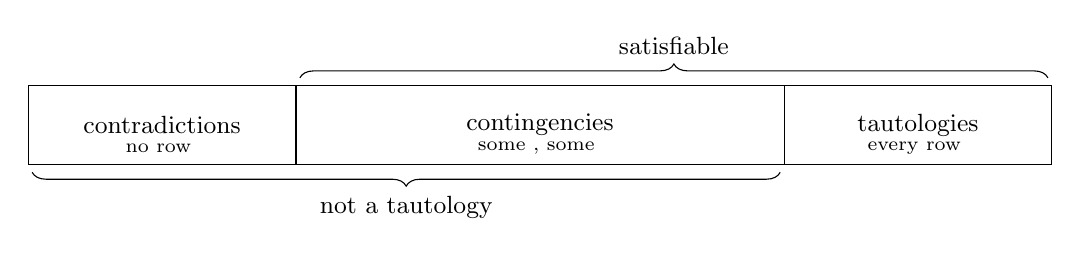
\begin{tikzpicture}[x=1cm,y=1cm]
  \draw (0,0) rectangle (3.4,1) node[midway,font=\small] {contradictions};
  \draw (3.4,0) rectangle (9.6,1) node[midway,font=\small] {contingencies};
  \draw (9.6,0) rectangle (13,1) node[midway,font=\small] {tautologies};
  \node[font=\scriptsize] at (1.7,0.2) {no row $\logT$};
  \node[font=\scriptsize] at (6.5,0.2) {some $\logT$, some $\logF$};
  \node[font=\scriptsize] at (11.3,0.2) {every row $\logT$};
  \draw[decorate,decoration={brace,amplitude=5pt}] (3.45,1.1) -- (12.95,1.1)
    node[midway,above=5pt,font=\small] {satisfiable};
  \draw[decorate,decoration={brace,amplitude=5pt,mirror}] (0.05,-0.1) -- (9.55,-0.1)
    node[midway,below=5pt,font=\small] {not a tautology};
\end{tikzpicture}
\caption{Every formula lands in exactly one box. ``Not a tautology'' covers two boxes, so it is not the same as ``contradiction''. Negating a formula swaps the two outer boxes and leaves a contingency a contingency.}
\end{figure}

\needspace{9\baselineskip}\textbf{Worked example.} Here are three formulas with every intermediate column written out.

\begin{center}
\begin{tabular}{cc|cc>{\bfseries}c|>{\bfseries}c|cc>{\bfseries}c}
\toprule
$P$ & $Q$ & $P\land Q$ & $\lnot(P\land Q)$ & $P\lor\lnot(P\land Q)$ & $(P\land Q)\land\lnot P$ & $\lnot P$ & $Q\land\lnot P$ & $P\to(Q\land\lnot P)$\\
\midrule
T & T & T & F & T & F & F & F & F\\
T & F & F & T & T & F & F & F & F\\
F & T & F & T & T & F & T & T & T\\
F & F & F & T & T & F & T & F & T\\
\bottomrule
\end{tabular}
\end{center}

$P\lor\lnot(P\land Q)$ is a tautology (all four rows $\logT$). $(P\land Q)\land\lnot P$ is a contradiction (all four $\logF$). $P\to(Q\land\lnot P)$ is a contingency: $(P{=}\logF,Q{=}\logT)$ satisfies it and $(P{=}\logT,Q{=}\logT)$ doesn't.

\textbf{What you have to show.} Learn this table. It tells you what a complete answer looks like for each kind of claim.

\begin{center}
\begin{tabularx}{\linewidth}{@{}lLL@{}}
\toprule
\textbf{Claim} & \textbf{To prove it} & \textbf{To disprove it}\\
\midrule
$p$ is satisfiable & one satisfying assignment (name it) & full table, no row $\logT$\\
$p$ is a tautology & full table, every row $\logT$ & one non-satisfying assignment, named explicitly\\
$p$ is a contradiction & full table, no row $\logT$ & one satisfying assignment\\
$p$ is a contingency & one satisfying \emph{and} one non-satisfying assignment & full table: all $\logT$ or all $\logF$\\
$p\equiv q$ & full table, the two columns identical & one assignment that satisfies one but not the other\\
\bottomrule
\end{tabularx}
\end{center}

The pattern: claims that say ``there is'' need one example; claims that say ``every'' or ``no'' need the whole table. Even when your table is on the page, write the witnessing assignment out in words.

\textbf{Where people slip.}
\begin{itemize}
  \item Skipping intermediate columns to save time. That's where evaluation mistakes hide, and a table with missing steps doesn't show your work.
  \item Calling a tautology a contingency (or the reverse) because one row was evaluated wrong. Recheck the $\to$ rows; that's where most errors are.
  \item Saying ``satisfiable'' and stopping. Give the assignment.
\end{itemize}

% ------------------------------------------------------------------
\subsection{Logical equivalence}

Two formulas can look nothing alike and still say the same thing.

\begin{notebox}
\textbf{Logical equivalence.} $p\equiv q$ when every assignment that satisfies one also satisfies the other. Equivalently, their final columns match row for row. (Another way to say it: $p\leftrightarrow q$ is a tautology.)
\end{notebox}

In this course you prove equivalence with a full truth table. Named rewriting laws (De Morgan's, distribution, and so on) are \emph{not} accepted as justification here. You may know them from elsewhere, and they're fine for guessing an answer, but the table is the proof.

\textbf{Worked example.} Is $\lnot(P\land Q)\equiv\lnot P\lor\lnot Q$?

\begin{center}
\begin{tabular}{cc|c>{\bfseries}c|cc>{\bfseries}c}
\toprule
$P$ & $Q$ & $P\land Q$ & $\lnot(P\land Q)$ & $\lnot P$ & $\lnot Q$ & $\lnot P\lor\lnot Q$\\
\midrule
T & T & T & F & F & F & F\\
T & F & F & T & F & T & T\\
F & T & F & T & T & F & T\\
F & F & F & T & T & T & T\\
\bottomrule
\end{tabular}
\end{center}

The two bold columns agree in every row, so yes, they're equivalent. Notice what the answer is made of: the table, plus the sentence saying the columns match.

When two formulas are \emph{not} equivalent, one row is enough, and you should name it. $P\to Q$ and $Q\to P$ differ at $(P{=}\logT,Q{=}\logF)$: that assignment satisfies $Q\to P$ but not $P\to Q$.

One more equivalence worth knowing because it describes how a conditional fails: $\lnot(P\to Q)\equiv P\land\lnot Q$. Check it with a four-row table yourself.

\textbf{Where people slip.}
\begin{itemize}
  \item Checking two or three rows and declaring the formulas equivalent. Matching on some rows proves nothing; every row has to match.
  \item Citing ``by De Morgan's law''. Here, that's an unsupported claim. Draw the table.
  \item Confusing $\equiv$ with $=$. $\equiv$ compares formulas across all assignments; $=$ is for sets and numbers.
\end{itemize}

% ------------------------------------------------------------------
\subsection{Converse, inverse, contrapositive}

Take a conditional $P\to Q$. Swap the parts, negate the parts, or do both, and you get three relatives:

\begin{center}
\begin{tabular}{lc}
\toprule
converse & $Q\to P$\\
inverse & $\lnot P\to\lnot Q$\\
contrapositive & $\lnot Q\to\lnot P$\\
\bottomrule
\end{tabular}
\qquad
\begin{tabular}{cc|>{\bfseries}cccc}
\toprule
$P$ & $Q$ & $P\to Q$ & $Q\to P$ & $\lnot P\to\lnot Q$ & $\lnot Q\to\lnot P$\\
\midrule
T & T & T & T & T & T\\
T & F & F & T & T & F\\
F & T & T & F & F & T\\
F & F & T & T & T & T\\
\bottomrule
\end{tabular}
\end{center}

Read the columns. The contrapositive matches the original in every row, so $P\to Q\equiv\lnot Q\to\lnot P$. The converse and the inverse each differ from the original (at $(\logT,\logF)$ and $(\logF,\logT)$), so neither is equivalent to it. They are equivalent to each other, though.

\begin{figure}[H]
\centering
\begin{tikzpicture}[x=5.2cm,y=2.1cm]
  \node[box] (o) at (0,1) {$P\to Q$\\[-2pt]\footnotesize original};
  \node[box] (c) at (1,1) {$Q\to P$\\[-2pt]\footnotesize converse};
  \node[box] (i) at (0,0) {$\lnot P\to\lnot Q$\\[-2pt]\footnotesize inverse};
  \node[box] (k) at (1,0) {$\lnot Q\to\lnot P$\\[-2pt]\footnotesize contrapositive};
  \draw[dashed] (o) -- node[lbl] {swap} (c);
  \draw[dashed] (o) -- node[lbl] {negate both} (i);
  \draw[dashed] (c) -- node[lbl] {negate both} (k);
  \draw[dashed] (i) -- node[lbl] {swap} (k);
  \draw[hl] (o) -- node[lbl,pos=0.3] {$\equiv$} (k);
  \draw[hl] (c) -- node[lbl,pos=0.3] {$\equiv$} (i);
\end{tikzpicture}
\caption{Thick diagonals join equivalent pairs (checked by the table above). Dashed sides are not equivalences.}
\end{figure}

\textbf{Worked example.} ``If a number is a multiple of 4, it's even.'' True for integers. Converse: ``if it's even, it's a multiple of 4'', false ($2$). Contrapositive: ``if it's odd, it's not a multiple of 4'', true, and it had to be, because it's equivalent to the original.

\textbf{Where people slip.} Assuming the converse because it ``feels'' like the same rule. People do this all the time outside class, too. If the course asks why two of these are or aren't equivalent, the answer is the table, not the vocabulary.

% ------------------------------------------------------------------
\subsection{Negation is not the opposite}

The negation of a statement is the statement that's true exactly when the original is false. That's often not the ``opposite'' that comes to mind.

\begin{itemize}
  \item ``He is tall'' negates to ``he is not tall'', not ``he is short''. Someone of medium height is neither tall nor short.
  \item ``$p$ is a tautology'' negates to ``$p$ is not a tautology'': some assignment fails to satisfy $p$. That's not the same as ``$p$ is a contradiction'' (see the figure in the satisfaction section).
  \item ``Every test case passed'' negates to ``at least one test case failed'', not ``every test case failed''.
  \item ``No integer squares to $-1$'' negates to ``some integer squares to $-1$''.
\end{itemize}

The general rule for claims about collections:

\begin{center}
\begin{tabular}{ll}
\toprule
\textbf{Claim} & \textbf{Negation}\\
\midrule
every $X$ is $Y$ & some $X$ is not $Y$\\
some $X$ is $Y$ & no $X$ is $Y$\\
no $X$ is $Y$ & some $X$ is $Y$\\
\bottomrule
\end{tabular}
\end{center}

Watch where you put the ``not''. The negation of ``some prime is even'' is ``no prime is even''. ``Some prime is not even'' is a true sentence, but it isn't the negation: it's true at the same time as the original ($2$ is an even prime, $3$ is an odd one).

\textbf{Where people slip.} Sticking ``not'' in the first grammatical spot that fits. Test your answer: exactly one of the original and your negation should be true, in every situation.

% ------------------------------------------------------------------
\subsection{Universal and existential claims}

Most claims you'll prove or disprove in this course are one of two kinds, and the kind tells you what kind of evidence you need.

\begin{notebox}
\textbf{Universal claim:} ``for every \dots'', ``all \dots'', ``no \dots'', ``if \dots\ then \dots''. Prove it by covering every case (one by one, or with a general argument). Disprove it with one counterexample.\\
\textbf{Existential claim:} ``there is \dots'', ``some \dots'', ``at least one \dots'', ``can'', ``possible''. Prove it with one example. Disprove it by showing every case fails.
\end{notebox}

Negating swaps the kind: the negation of a universal claim is existential, and the other way around. That's why one counterexample is enough to sink a universal claim.

The tricky part is that a lot of claims hide their quantifier inside a definition. Unpack it before you decide what evidence to give.

\begin{center}
\begin{tabularx}{\linewidth}{@{}lLc@{}}
\toprule
\textbf{Claim} & \textbf{What it says once you unpack it} & \textbf{Kind}\\
\midrule
$A\subseteq B$ & every member of $A$ is a member of $B$ & universal\\
$A=B$ & every member of either set is in the other & universal\\
$A\cap B=\varnothing$ & nothing is a member of both & universal\\
$p$ is a tautology & every assignment satisfies $p$ & universal\\
$p$ is not satisfiable & no assignment satisfies $p$ & universal\\
$n$ is prime & no $m$ with $1<m<n$ divides $n$ & universal\\
\midrule
$A\not\subseteq B$ & some member of $A$ isn't in $B$ & existential\\
$x\in\mathbb{Q}$ & there are integers $p,q$ ($q\neq0$) with $x=\frac pq$ & existential\\
$x\in\{n^2\mathrel{|} n\in\mathbb{Z}\}$ & some integer $n$ has $n^2=x$ & existential\\
$p$ is satisfiable & some assignment satisfies $p$ & existential\\
$p$ is a contingency & some assignment satisfies $p$ and some doesn't & existential\\
\bottomrule
\end{tabularx}
\end{center}

\textbf{Worked example.} ``$\{1,4,8\}\subseteq\{n^2\mathrel{|} n\in\mathbb{Z}\}$.'' Universal, so a single counterexample settles it: $8$ is in the left set and isn't a perfect square. False. Compare ``$9\in\{n^2\mathrel{|} n\in\mathbb{Z}\}$'': existential, so one witness settles it: $n=3$. True. (Membership in a set-builder set is existential, as in the sets chapter.)

\textbf{Where people slip.}
\begin{itemize}
  \item Proving a universal claim with one example. Examples prove existential claims only.
  \item Disproving an existential claim with one non-example. You need to rule out everything.
\end{itemize}

% ------------------------------------------------------------------
\subsection{Vacuous truth}

Here's a claim: ``Every member of $\{n\in\mathbb{Z}\mathrel{|} n^2<0\}$ is a prime number.'' True or false?

It's true. The set is empty, so there's nothing to check. To show it's false you'd need a counterexample, which would have to be a member of the set that isn't prime, and there are no members at all. A universal claim with no counterexample is true.

\begin{notebox}
\textbf{Vacuous truth.} A universal claim whose premise nothing can satisfy is true, whatever the conclusion says.
\end{notebox}

This is the same thing as the bottom two rows of the $\to$ table. When the premise is false, the conditional is true.

More examples:
\begin{itemize}
  \item $\varnothing\subseteq A$ for every set $A$. ``Every member of $\varnothing$ is in $A$'' has nothing to check.
  \item An empty dishwasher is ``all clean'' and also ``all dirty''. Both are vacuously true.
  \item $(P\land\lnot P)\to Q$ is a tautology. The premise is never satisfied, so no row can break it.
  \item The existential version flips: ``\emph{some} member of $\{n\in\mathbb{Z}\mathrel{|} n^2<0\}$ is prime'' is false, since there's no member to be the example.
\end{itemize}

\textbf{Where people slip.} Answering ``false'' or ``doesn't make sense'' because the conclusion sounds wrong, or because there's nothing to talk about. If the premise can't happen, the universal claim is true. Say so, and say why: ``vacuously true, since nothing satisfies the premise.''

% ------------------------------------------------------------------
\subsection{Practice}

None of these come from homework. For anything that needs a table, write every intermediate column.

\begin{enumerate}[label=\textbf{\arabic*.},leftmargin=1.8em,itemsep=0.35em]
  \item Proposition, expression, or neither?\\
  (a) ``$x+3$ is even'' \quad (b) ``the set of odd primes'' \quad (c) ``Close the door.''\\ (d) $\{1,2\}\cup\{3\}$ \quad (e) $\{1,2\}\subseteq\{3\}$ \quad (f) ``Is 7 prime?''
  \item Atoms: $R$ = ``it rains'', $G$ = ``the game is on'', $T$ = ``we have tickets'', $I$ = ``we get in''. Translate:\\
  (a) The game is on unless it rains. \quad (b) The game is on only if it isn't raining.\\
  (c) Having tickets is necessary for getting in. \quad (d) Rain is sufficient for the game to be off.\\
  (e) It's raining, but the game is on. \quad (f) We get in if and only if we have tickets and the game is on.\\
  (g) It's neither raining nor is the game on.
  \item (a) Does $(P{=}\logT,Q{=}\logF,R{=}\logT)$ satisfy $(P\to Q)\lor(Q\oplus R)$?\\
  (b) Does $(P{=}\logF,Q{=}\logF,R{=}\logF)$ satisfy $\lnot(P\lor R)\leftrightarrow Q$?
  \item Classify each as tautology, contradiction, or contingency, with the evidence the obligation table asks for:\\
  (a) $(P\to Q)\lor(Q\to P)$ \quad (b) $(P\leftrightarrow Q)\land(P\oplus Q)$ \quad (c) $(P\land\lnot Q)\to\lnot P$\\
  (d) $((P\to Q)\land\lnot Q)\to\lnot P$ \quad (e) $(P\lor Q)\to(P\lor R)$
  \item Equivalent or not? Prove your answer.\\
  (a) $\lnot(P\leftrightarrow Q)$ and $P\oplus Q$ \quad (b) $P\to(Q\to R)$ and $(P\land Q)\to R$\\
  (c) $(P\to R)\land(Q\to R)$ and $(P\land Q)\to R$ \quad (d) $\lnot(P\land Q)$ and $\lnot P\land\lnot Q$
  \item For integers: ``If $n$ is divisible by 6, then $n$ is even.'' Write the converse, inverse and contrapositive, and say which of the four statements are true.
  \item Negate each (a real negation, not an opposite):\\
  (a) Every bus today was late. \quad (b) Some password on the list is shorter than 8 characters.\\
  (c) The formula $p$ is a tautology. \quad (d) No square of an integer is negative.
  \item Say whether each claim is universal or existential (after unpacking), then whether it's true:\\
  (a) $\{4,9\}\subseteq\{n^2\mathrel{|} n\in\mathbb{Z}\}$ \quad (b) $12\in\{n^2-n\mathrel{|} n\in\mathbb{Z}\}$ \quad (c) $P\land\lnot P$ is not satisfiable\\
  (d) $\{1,2\}\neq\{2,1,1\}$ \quad (e) $P\to Q$ is a contingency
  \item True or false?\\
  (a) Every member of $\{n\in\mathbb{N}\mathrel{|} n<0\}$ is odd. \quad (b) Some member of $\{n\in\mathbb{N}\mathrel{|} n<0\}$ is odd.\\
  (c) Every truth assignment that satisfies $P\land\lnot P$ also satisfies $Q$.\\
  (d) Every subset $A$ of $\{7\}$ with $|A|=2$ is empty. \quad (e) ``If 3 is even, then 3 is prime.''
  \item (a) How many rows does a truth table with atoms $P,Q,R,S$ have?\\
  (b) A formula in $P$ and $Q$ has a final column of four $\logT$/$\logF$ entries. How many different final columns are possible? How many belong to tautologies, contradictions, contingencies?
  \item One friend says ``$P$ only if $Q$'' means ``if $Q$ then $P$''. Another says it means ``$Q$ is necessary for $P$''. Who's right? Back it up with a table.
\end{enumerate}

% ------------------------------------------------------------------
\subsection{Answers}

Every table and classification here was checked by brute force.

\begin{enumerate}[label=\textbf{\arabic*.},leftmargin=1.8em,itemsep=0.45em]
  \item (a) Proposition: it's true or false once $x$ has a value. (b) Expression: it names a set. (c) Neither: a command. (d) Expression: it names the set $\{1,2,3\}$. (e) Proposition (a false one, since $1\notin\{3\}$). (f) Neither: a question.
  \item (a) $G\lor R$. (b) $G\to\lnot R$. (c) $I\to T$ (necessary goes in the conclusion). (d) $R\to\lnot G$. (e) $R\land G$. (f) $I\leftrightarrow(T\land G)$. (g) $\lnot R\land\lnot G$.
  \item (a) $P\to Q$ is $\logT\to\logF=\logF$. $Q\oplus R$ is $\logF\oplus\logT=\logT$. So $\logF\lor\logT=\logT$. Yes, it satisfies the formula.
  (b) $P\lor R=\logF$, so $\lnot(P\lor R)=\logT$, and $\logT\leftrightarrow\logF=\logF$. No.
  \item Parts (a) and (b), with every intermediate column:

  \smallskip\begin{tabular}{cc|cc>{\bfseries}c|cc>{\bfseries}c}
  \toprule
  $P$ & $Q$ & $P\to Q$ & $Q\to P$ & (a) & $P\leftrightarrow Q$ & $P\oplus Q$ & (b)\\
  \midrule
  T & T & T & T & T & T & F & F\\
  T & F & F & T & T & F & T & F\\
  F & T & T & F & T & F & T & F\\
  F & F & T & T & T & T & F & F\\
  \bottomrule
  \end{tabular}\par\smallskip

  (a) \textbf{Tautology}: every row is $\logT$. (b) \textbf{Contradiction}: no row is $\logT$. The two parts can never agree, since $\oplus$ is $\logT$ exactly where $\leftrightarrow$ is $\logF$.

  Parts (c) and (d):

  \smallskip\begin{tabular}{cc|ccc>{\bfseries}c|cc>{\bfseries}c}
  \toprule
  $P$ & $Q$ & $\lnot P$ & $\lnot Q$ & $P\land\lnot Q$ & (c) & $P\to Q$ & $(P\to Q)\land\lnot Q$ & (d)\\
  \midrule
  T & T & F & F & F & T & T & F & T\\
  T & F & F & T & T & F & F & F & T\\
  F & T & T & F & F & T & T & F & T\\
  F & F & T & T & F & T & T & T & T\\
  \bottomrule
  \end{tabular}\par\smallskip

  (c) \textbf{Contingency}: $(P{=}\logF,Q{=}\logT)$ satisfies it and $(P{=}\logT,Q{=}\logF)$ doesn't. (d) \textbf{Tautology}: every row is $\logT$.

  (e) \textbf{Contingency}, and two assignments are all you need. $(P{=}\logF,Q{=}\logT,R{=}\logF)$: the premise $P\lor Q$ is $\logT$ and the conclusion $P\lor R$ is $\logF$, so it isn't satisfied. $(P{=}\logT,Q{=}\logT,R{=}\logT)$: both sides are $\logT$, so it is.
  \item (a) \textbf{Equivalent.} The full table:

  \smallskip\begin{tabular}{cc|c>{\bfseries}c>{\bfseries}c}
  \toprule
  $P$ & $Q$ & $P\leftrightarrow Q$ & $\lnot(P\leftrightarrow Q)$ & $P\oplus Q$\\
  \midrule
  T & T & T & F & F\\
  T & F & F & T & T\\
  F & T & F & T & T\\
  F & F & T & F & F\\
  \bottomrule
  \end{tabular}\par\smallskip

  The bold columns match in all four rows.

  (b) \textbf{Equivalent.} Eight rows this time:

  \smallskip\begin{tabular}{ccc|c>{\bfseries}c|c>{\bfseries}c}
  \toprule
  $P$ & $Q$ & $R$ & $Q\to R$ & $P\to(Q\to R)$ & $P\land Q$ & $(P\land Q)\to R$\\
  \midrule
  T & T & T & T & T & T & T\\
  T & T & F & F & F & T & F\\
  T & F & T & T & T & F & T\\
  T & F & F & T & T & F & T\\
  F & T & T & T & T & F & T\\
  F & T & F & F & T & F & T\\
  F & F & T & T & T & F & T\\
  F & F & F & T & T & F & T\\
  \bottomrule
  \end{tabular}\par\smallskip

  The bold columns match in all eight rows. Both formulas fail only when $P$ and $Q$ are true and $R$ is false.

  (c) \textbf{Not equivalent.} At $(P{=}\logT,Q{=}\logF,R{=}\logF)$: $P\to R$ is $\logF$, so the left side is $\logF$; $P\land Q$ is $\logF$, so the right side is $\logT$. That assignment satisfies the right formula but not the left. One row is enough.

  (d) \textbf{Not equivalent.} At $(P{=}\logT,Q{=}\logF)$: $\lnot(P\land Q)=\logT$ but $\lnot P\land\lnot Q=\logF$.
  \item Original: if $6\mid n$ then $n$ is even. True (a multiple of 6 is a multiple of 2).
  Converse: if $n$ is even then $6\mid n$. False, $n=2$.
  Inverse: if $6\nmid n$ then $n$ is odd. False, $n=2$ again.
  Contrapositive: if $n$ is odd then $6\nmid n$. True. It's equivalent to the original, so it had to be.
  \item (a) At least one bus today was not late. (b) Every password on the list has at least 8 characters. (c) Some truth assignment doesn't satisfy $p$. (Not ``$p$ is a contradiction''.) (d) Some integer has a negative square.
  \item (a) Universal (every member of the left is a square). True: $4=2^2$, $9=3^2$.
  (b) Existential (some integer $n$ gives $n^2-n=12$). True: $n=4$ works ($n=-3$ also does).
  (c) Universal (no assignment satisfies it). True: $P\land\lnot P$ is $\logF$ in both rows.
  (d) Existential (some member of one set isn't in the other). False: both sets are $\{1,2\}$.
  (e) Existential (one satisfying and one non-satisfying assignment). True: $(\logT,\logT)$ satisfies it, $(\logT,\logF)$ doesn't.
  \item (a) True, vacuously: no natural number is negative, so there's nothing to be a counterexample.
  (b) False: an existential claim needs a member to point at, and there isn't one.
  (c) True, vacuously: no assignment satisfies $P\land\lnot P$.
  (d) True, vacuously: $\{7\}$ has no two-member subsets.
  (e) True: the premise is false, so the conditional is true.
  \item (a) $2^4=16$.
  (b) Each of the four rows independently gets $\logT$ or $\logF$, so $2^4=16$ possible columns. Exactly one is all $\logT$ (tautologies), exactly one is all $\logF$ (contradictions), and the other $14$ are contingencies. Any two formulas with the same column are equivalent, so up to equivalence there are only 16 formulas in two variables.
  \item The second friend. ``$P$ only if $Q$'' is $P\to Q$, and ``$Q$ is necessary for $P$'' is also $P\to Q$, so they're literally the same formula. ``If $Q$ then $P$'' is $Q\to P$, the converse.

  \smallskip\begin{tabular}{cc|cc}
  \toprule
  $P$ & $Q$ & $P\to Q$ & $Q\to P$\\
  \midrule
  T & T & T & T\\
  T & F & F & T\\
  F & T & T & F\\
  F & F & T & T\\
  \bottomrule
  \end{tabular}\par\smallskip

  The columns differ at $(P{=}\logT,Q{=}\logF)$ (and at $(P{=}\logF,Q{=}\logT)$), so the first friend's version is not equivalent.
\end{enumerate}

\clearpage
\section{Proofs: the constrained style}
\label{sec:proofs}

% ---------------------------------------------------------------------------
% Fitch-style proof drawing macros (local to this chapter, \prf prefix).
%   \prfstart                          origin node (p0); call first
%   \prfline{name}{prev}{depth}{num}{text}{rule}
%        one proof line, placed under node {prev}; depth 0 = outside every
%        subproof; the rule label sits right-aligned in its own column
%   \prfscope{first}{last}{depth}{bar}
%        vertical scope bar from line {first} to line {last} at {depth},
%        plus the short horizontal "assumption" bar under {first}
% ---------------------------------------------------------------------------
\newcommand{\prfgap}{0.5cm}
\newcommand{\prfstart}{\node[inner sep=0pt,minimum size=0pt] (p0) at (0,0) {};}
\newcommand{\prfline}[6]{%
  \node[anchor=north west,inner sep=2pt,font=\small,align=flush left,
        text width=\dimexpr 10.9cm-#3\dimexpr\prfgap\relax\relax]
    (#1t) at ($(0,0 |- #2.south)+(0.7cm+#3*\prfgap,-1.2pt)$) {#5};
  \node[anchor=north east,inner sep=2pt,font=\small,align=flush right,text width=4.3cm]
    (#1r) at ($(0,0 |- #1t.north)+(16.3cm,0)$) {#6};
  \node[anchor=north west,inner sep=2pt,font=\small] at (0,0 |- #1t.north) {#4};
  \node[fit=(#1t)(#1r),inner sep=0pt] (#1) {};}
\newcommand{\prfscope}[4]{%
  \draw ($(0,0 |- #1.north)+(0.7cm+#3*\prfgap-0.16cm,-1.2pt)$)
     -- ($(0,0 |- #2.south)+(0.7cm+#3*\prfgap-0.16cm,1.2pt)$);
  \draw ($(0,0 |- #1t.south)+(0.7cm+#3*\prfgap-0.16cm,0)$) -- ++(#4,0);}
\newcommand{\prfqed}{\ $\mdlgwhtsquare$}

This is the part of Test 1 where points actually get lost. Computing $A-B$ or filling in a truth table is mechanical. A constrained proof isn't: you have to pick a move, justify it with exactly the right rule, and not take a step that only \emph{feels} valid. The good news is that the moves are few and the choice of move is almost always forced by what the goal looks like. This chapter is about learning to see that.

Everything here comes from notes \S3.1--3.13 and the subset material in \S2.5.1. Every claim in this chapter was written fresh for this guide, and each was checked by brute force over all subsets of $\{0,1,2,3\}$.

\subsection{What counts as a proof in this course}

A proof is a chain of reasoning where every step follows logically from things you already have. That's it. How much detail you show, and what format you use, varies a lot, and the notes sort proofs into three kinds:

\begin{itemize}
  \item A \emph{formal proof} uses a fixed, small set of logical rules and a rigid format, like source code for an argument. Logicians write these when they're studying logic itself or feeding proofs to a computer.
  \item An \emph{informal proof} is everything else: textbook proofs, papers, the stuff on a whiteboard. Still airtight, but any valid rule is allowed and the writer decides how much detail the reader needs. Informal doesn't mean sloppy.
  \item A \emph{constrained proof} is the middle ground this course uses for now. It's written in ordinary English sentences, but you may only use the rules and definitions on the list you're given, at most one rule (plus at most one definition) per line, and you must name what you used.
\end{itemize}

Why bother with the constrained style? Because it makes every step checkable. In an informal proof, ``clearly $x\notin B$'' can hide a broken inference. In a constrained proof, that line has to carry a rule name, and the grader can hold it up against the rule's exact wording. So can you.

Here's the mental model that makes the rest of this chapter click. Think of a proof as a game. The \emph{goal} (what you're trying to show) has a shape, and that shape tells you your opening move. The facts you're \emph{holding} also have shapes, and they tell you what you can do next. You win when what you hold matches the goal.

\subsection{The toolkit}

\subsubsection{Five definitions}

For set proofs you'll get these definitions, and only these. Each one turns a statement about sets into a statement about a single member $x$, which is what makes the rules usable.

\begin{center}
\begin{tabularx}{\linewidth}{@{}l>{\raggedright\arraybackslash}p{6.6cm}L@{}}
\toprule
\textbf{Cite as} & \textbf{Definition} & \textbf{Logic inside it}\\
\midrule
def.\ of compl. & $x\in\overline{A}$ means $x\notin A$ & a ``not'' (needs a universe $\mathcal{U}$)\\
def.\ of $\cap$ & $x\in A\cap B$ means $x\in A$ and $x\in B$ & an ``and''\\
def.\ of $\cup$ & $x\in A\cup B$ means $x\in A$ or $x\in B$ (or both) & an inclusive ``or''\\
def.\ of $-$ & $x\in A-B$ means $x\in A$ and $x\notin B$ & an ``and'' with a ``not''\\
def.\ of $\subseteq$ & $A\subseteq B$ means for every $x\in A$, we also have $x\in B$ & a universal claim\\
\bottomrule
\end{tabularx}
\end{center}

Definitions work in both directions. ``$x\in A\cap B$, so $x\in A$ and $x\in B$'' is def.\ of $\cap$, and so is ``$x\in A$ and $x\in B$, so $x\in A\cap B$''. You'll use both directions in almost every proof: once to \emph{unpack} what you were given, once to \emph{pack up} what you need.

You are not allowed to use known set facts that aren't on the list. ``Obviously $A\subseteq A\cup B$'' or a De Morgan law can't be cited; if you need one, you prove that piece with the rules.

\subsubsection{The rules}

Seven rules, plus one way to disprove things. Learn the names \emph{and} the abbreviations; the abbreviation is what goes in the parentheses at the end of each line.

\begin{longtable}{@{}>{\raggedright\arraybackslash}p{3.3cm}>{\raggedright\arraybackslash}p{6.5cm}>{\raggedright\arraybackslash}p{5.8cm}@{}}
\toprule
\textbf{Rule (cite as)} & \textbf{What it says} & \textbf{Reach for it when}\\
\midrule
\endhead
Universal Introduction (univ.\ intro.) & Assume an object with property $P$, give it a currently unused name, prove it has $Q$. Then every object with $P$ has $Q$. & The goal says ``every'', ``for any'', or is $X\subseteq Y$.\\
\addlinespace
Implication Introduction (impl.\ intro.) & Assume $X$, prove $Y$. Then ``if $X$, then $Y$''. & The goal is an if--then.\\
\addlinespace
Application (appl.) & You know everything with $P$ has $Q$, and you have an object with $P$. Then it has $Q$. & You hold $A\subseteq B$ \emph{and} a member of $A$.\\
\addlinespace
Weakening (weak.) & From $X$, conclude ``$X$ or $Y$'' for any $Y$ at all. & The goal is an ``or'' (often $x\in A\cup B$).\\
\addlinespace
Disjunctive Syllogism (disj.\ syll.) & From ``$X$ or $Y$'' and ``$X$ is false'', conclude $Y$. & You hold an ``or'' and one side is already ruled out.\\
\addlinespace
Proof by Cases (pf.\ by cases) & From ``$X$ or $Y$'', a subproof assuming $X$ that reaches $Z$, and a subproof assuming $Y$ that reaches $Z$: conclude $Z$. & You hold an ``or'' and neither side is ruled out.\\
\addlinespace
Proof by Contradiction (contrad.) & Assume $X$ in a subproof, prove some $Y$ is both true and false. Then $X$ is false. & The goal is a ``not'': $x\notin S$, or $x\in\overline{A}$ via $x\notin A$.\\
\midrule
Proof by Counterexample & Name a specific object, show it has $P$, show it lacks $Q$. Then ``everything with $P$ has $Q$'' is false. & You suspect the claim is false.\\
\bottomrule
\end{longtable}

\begin{notebox}
\textbf{Two small slips in the notes' summary list.} In the \S3.13 summary, Weakening is listed with the alias ``$\vee$-Elimination''. Section~3.6 has it right: Weakening is \emph{$\vee$-Introduction} (it creates an ``or''); $\vee$-Elimination is Proof by Cases (it uses one up). And the guidelines say to mark a contradiction subproof ``towards an introduction''; the phrase you want is ``Suppose \emph{towards a contradiction} that \dots''.
\end{notebox}

\subsection{House rules for writing one}

These are the constrained-proof guidelines from \S3.13, said plainly. Graders check every one.

\begin{enumerate}
  \item \textbf{Write the claim first}, before the proof starts.
  \item \textbf{Every proof and subproof opens with its assumptions.} A univ.\ intro.\ or impl.\ intro.\ opening also states its goal, like ``(Goal: $A-C\subseteq B$)''. You may merge the ``for any sets'' and the ``if'' into one opening line. A contradiction subproof says so: ``Suppose towards a contradiction that \dots''.
  \item \textbf{One step, one rule, and at most one definition.} Each non-assumption line uses at most one rule and at most one definition, all from the list you're given. ``(appl., def.\ of $\subseteq$)'' is fine. ``(appl., def.\ of $\subseteq$, def.\ of $\cup$)'' is two definitions, so it's two lines.
  \item \textbf{Name the rule or definition} on every line.
  \item \textbf{Name the facts you used.} ``Since $x\in A$ and $A\subseteq B$, \dots'' rather than just ``so $x\in B$''. If the fact is the line right above, ``so'', ``thus'' or ``hence'' is enough. If you apply a theorem, name it.
  \item \textbf{Restate after a subproof closes.} After univ.\ intro., say what you assumed and what you proved: ``We chose an arbitrary $x\in A$ and proved $x\in B$, so \dots''. After contrad., say what you assumed \emph{and} the two facts that clashed.
  \item \textbf{End with} $\mdlgwhtsquare$.
\end{enumerate}

\subsubsection{How to read the diagrams in this chapter}

The proofs below are drawn Fitch-style. Each line has a number on the left and its justification on the right. A vertical bar marks how long a subproof lasts; the short horizontal bar sits under the line that opens it (its assumption). When a bar ends, that subproof is closed. You don't have to draw bars on the test (indenting is enough), but picturing them is the fastest way to keep scope straight.

Here's the skeleton that most Test 1 proofs follow. If the goal is $X\subseteq Y$, you can write five of these lines before you've thought about anything.

\begin{center}
\begin{tikzpicture}
  \prfstart
  \prfline{s1}{p0}{1}{1}{Let $A,B,\dots$ be sets and assume [hypothesis].}{(Goal: $X\subseteq Y$)}
  \prfline{s2}{s1}{2}{2}{Let $x\in X$.}{(Subgoal: $x\in Y$)}
  \prfline{s3}{s2}{2}{3}{[unpack $x\in X$ with its definition]}{(def.\ of $\cap$ / $\cup$ / $-$ / compl.)}
  \prfline{s4}{s3}{2}{4}{[feed a \emph{member} into the hypothesis]}{(appl., def.\ of $\subseteq$)}
  \prfline{s5}{s4}{2}{5}{[build $x\in Y$ from the pieces]}{(def.\ / weak.\ / disj.\ syll.\ / \dots)}
  \prfline{s6}{s5}{1}{6}{We chose an arbitrary $x\in X$ and proved $x\in Y$, so $X\subseteq Y$.}{(univ.\ intro., def.\ of $\subseteq$)}
  \prfline{s7}{s6}{0}{7}{We chose sets $A,B,\dots$ with [hypothesis] and proved $X\subseteq Y$, which proves the claim.\prfqed}{(univ.\ intro.)}
  \prfscope{s1}{s6}{1}{3.4cm}
  \prfscope{s2}{s5}{2}{1.4cm}
\end{tikzpicture}
\end{center}

Line 2 is the heart of univ.\ intro.: pick a nameless representative. $x$ isn't any particular member of $X$; it's \emph{a} member you know nothing else about. Whatever you prove about it, you could prove about every member, which is why line 6 gets to say ``so $X\subseteq Y$''. The name has to be fresh: if $x$ already meant something earlier, you'd be smuggling in extra facts. Lowercase for members, uppercase for sets.

\subsection{Scope: subproofs are temporary worlds}

Every subproof is a ``what if''. Inside it you get to assume something extra, and you can use everything from the outer proof too. Facts flow \emph{in}. But anything you derive inside depends on that extra assumption, so when the subproof closes, those facts die with it. The only thing that gets out is the conclusion of the rule that closes the subproof.

\begin{center}
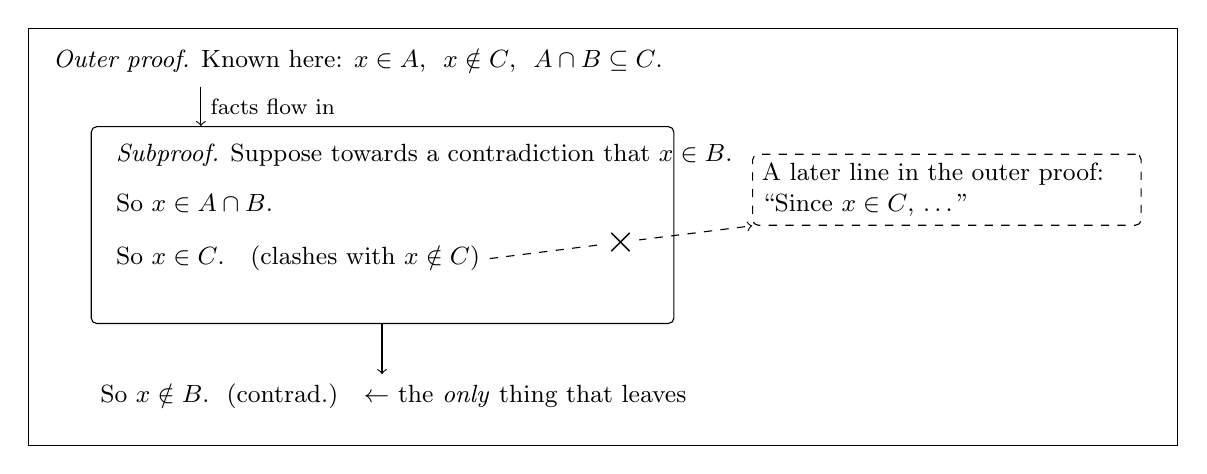
\begin{tikzpicture}[font=\small]
  \node[draw,rectangle,minimum width=14.6cm,minimum height=5.3cm,anchor=north west] (outer) at (0,0) {};
  \node[anchor=north west,align=left] at (0.2,-0.15) {\textit{Outer proof.} Known here: $x\in A$,\ \ $x\notin C$,\ \ $A\cap B\subseteq C$.};
  \draw[->] (2.2,-0.75) -- (2.2,-1.25) node[midway,right,font=\footnotesize] {facts flow in};
  \node[draw,rounded corners=2pt,minimum width=7.4cm,minimum height=2.5cm,anchor=north west] (inner) at (0.8,-1.25) {};
  \node[anchor=north west,align=left] (i1) at (1.0,-1.35) {\textit{Subproof.} Suppose towards a contradiction that $x\in B$.};
  \node[anchor=north west,align=left] (i2) at (1.0,-2.0) {So $x\in A\cap B$.};
  \node[anchor=north west,align=left] (i3) at (1.0,-2.65) {So $x\in C$.\quad (clashes with $x\notin C$)};
  \draw[->] (4.5,-3.75) -- (4.5,-4.4);
  \node[anchor=north west,align=left] (out) at (0.8,-4.4) {So $x\notin B$.\ \ (contrad.)\quad $\leftarrow$ the \emph{only} thing that leaves};
  \node[draw,dashed,rounded corners=2pt,align=left,text width=4.7cm,anchor=north west] (later) at (9.2,-1.6)
     {A later line in the outer proof: ``Since $x\in C$, \dots''};
  \draw[->,dashed] (i3.east) -- node[pos=0.5,fill=white,inner sep=1pt,font=\Large] {$\times$} (later.south west);
\end{tikzpicture}
\end{center}

The dashed arrow is the mistake. $x\in C$ was only true \emph{if} $x\in B$, and the whole point of the subproof was to show that $x\in B$ is false. Citing $x\in C$ outside would be citing something you now know rests on a false assumption. Same story with cases: what you prove inside Case 1 was only true in Case 1. Proof by Cases lets you export one thing, the common conclusion $Z$ you reached in \emph{both} cases.

\subsection{Choosing your move}

Most of being good at these is reading two things: the shape of your goal, and the shape of what you hold. Start from the goal, because it decides the frame of the whole proof.

\begin{figure}[H]
\centering
\begin{tikzpicture}
  \node[softbox,text width=6.2cm,anchor=north west] (start) at (-2.9,0) {Look at your \textbf{goal}. What shape is it?};
  \matrix[matrix of nodes,anchor=north west,column sep=0.75cm,row sep=0.16cm,
    nodes={draw,rectangle,align=left,font=\small,inner sep=3pt},
    column 1/.style={nodes={text width=4.1cm}},
    column 2/.style={nodes={text width=9.1cm}}] (g) at (-2.0,-0.8) {
    ``every \dots'', ``for any \dots'' & univ.\ intro.: name a fresh, arbitrary object with the premise property; write the Goal.\\
    ``if $P$, then $Q$'' & impl.\ intro.: assume $P$, make $Q$ the goal. With ``for any'', fold both into one opening line.\\
    $X\subseteq Y$ & It's universal (def.\ of $\subseteq$). Let $x\in X$, subgoal $x\in Y$; close with (univ.\ intro., def.\ of $\subseteq$).\\
    $X=Y$ & Two $\subseteq$ subproofs: $X\subseteq Y$, then $Y\subseteq X$.\\
    $x\in A\cap B$ & Get $x\in A$ and $x\in B$ separately, then (def.\ of $\cap$).\\
    $x\in A\cup B$ & Get \emph{one} side, then (weak.) and (def.\ of $\cup$). Aim at the side you can reach.\\
    $x\in A-B$ & Get $x\in A$ and $x\notin B$, then (def.\ of $-$).\\
    $x\in\overline{A}$ & Get $x\notin A$, then (def.\ of compl.).\\
    $x\notin S$, or ``not $P$'' & contrad.: ``Suppose towards a contradiction that $x\in S$'', then hunt for a fact and its opposite.\\
    You suspect it's false & Counterexample: specific sets that make the premise true and the conclusion false.\\
  };
  \draw (-2.4,0 |- start.south) -- (-2.4,0 |- g-10-1.west);
  \foreach \i in {1,...,10} { \draw[->] (-2.4,0 |- g-\i-1.west) -- (g-\i-1.west); \draw[->] (g-\i-1.east) -- (g-\i-2.west); }
\end{tikzpicture}
\caption{Goal shape $\to$ first move. Work top-down: the outer shape first (``for any \dots, if \dots, then $X\subseteq Y$''), then the shape of each subgoal as it appears.}
\label{fig:goalchooser}
\end{figure}

Once the frame is up, you're inside a subproof holding some facts. Now the question flips: what can I \emph{do} with what I have?

\begin{figure}[H]
\centering
\begin{tikzpicture}[
  hold/.style={draw,rectangle,align=left,font=\small,text width=3.3cm,inner sep=3pt},
  move/.style={draw,rectangle,align=left,font=\small,text width=6.6cm,inner sep=3pt},
  ask/.style={draw,diamond,aspect=2.3,align=center,font=\footnotesize,inner sep=1pt,text width=2.3cm},
  yn/.style={font=\footnotesize,fill=white,inner sep=1pt}]
  \node[font=\small\itshape] at (1.8,0.55) {You hold \dots};
  \node[font=\small\itshape] at (12.4,0.55) {Your move};
  \node[hold] (h1) at (1.8,0) {$x\in A\cap B$};
  \node[move] (m1) at (12.4,0) {Split it: $x\in A$, and $x\in B$. (def.\ of $\cap$)};
  \node[hold] (h2) at (1.8,-0.85) {$x\in A-B$};
  \node[move] (m2) at (12.4,-0.85) {Split it: $x\in A$, and $x\notin B$. (def.\ of $-$)};
  \node[hold] (h3) at (1.8,-1.7) {$x\in\overline{A}$};
  \node[move] (m3) at (12.4,-1.7) {$x\notin A$. (def.\ of compl.)};
  \foreach \i in {1,2,3} \draw[->] (h\i) -- (m\i);
  % or
  \node[hold] (h4) at (1.8,-3.35) {$x\in A\cup B$, so ``$x\in A$ or $x\in B$'' (def.\ of $\cup$)};
  \node[ask] (q4) at (6.4,-3.35) {Is one side already known false?};
  \node[move] (y4) at (12.4,-2.75) {disj.\ syll.: conclude the other side.};
  \node[move] (n4) at (12.4,-3.95) {pf.\ by cases: one subproof per side; reach the same $Z$ in both.};
  \draw[->] (h4) -- (q4);
  \draw[->] (q4.north) |- node[yn,pos=0.75] {yes} (y4.west);
  \draw[->] (q4.south) |- node[yn,pos=0.75] {no} (n4.west);
  % subset
  \node[hold] (h5) at (1.8,-6.0) {A subset fact $A\subseteq B$};
  \node[ask] (q5) at (6.4,-6.0) {Do you have a \emph{member} of $A$?};
  \node[move] (y5) at (12.4,-5.4) {appl.: that member is in $B$. (appl., def.\ of $\subseteq$)};
  \node[move] (n5) at (12.4,-6.6) {You only have $x\notin A$? Then \textbf{nothing} follows about $B$. Look for another route.};
  \draw[->] (h5) -- (q5);
  \draw[->] (q5.north) |- node[yn,pos=0.75] {yes} (y5.west);
  \draw[->] (q5.south) |- node[yn,pos=0.75] {no} (n5.west);
  % contradiction
  \node[hold] (h6) at (1.8,-8.15) {Some $Y$ and also not-$Y$, inside a subproof that assumed $X$};
  \node[move] (m6) at (12.4,-8.15) {Close it: $X$ is false. Name $X$ and both clashing facts. (contrad.)};
  \draw[->] (h6) -- (m6);
  \node[hold] (h7) at (1.8,-9.45) {A fact from inside a closed subproof};
  \node[move] (m7) at (12.4,-9.45) {Unusable. Only the closing line's conclusion survives.};
  \draw[->] (h7) -- (m7);
\end{tikzpicture}
\caption{What you hold $\to$ next move. The two diamonds are where most wrong steps come from: using disj.\ syll.\ without a side ruled out, and using a subset fact without a member.}
\label{fig:holdchooser}
\end{figure}

\subsubsection{The classic invalid step}

This one deserves its own heading because it's the single most common way to wreck a proof. You hold $x\notin A$ and $A\subseteq B$, and you write ``so $x\notin B$ (appl.)''.

It's invalid. $A\subseteq B$ talks about members of $A$: every one of them is in $B$. It says nothing at all about things outside $A$. Picture $A$ as a small circle inside a big circle $B$. A point outside the small circle can easily sit inside the big one. Application needs an object \emph{with} the property; $x\notin A$ is the object \emph{without} it.

If you genuinely need $x\notin B$, the route is a contradiction subproof: suppose $x\in B$, and find something that breaks. Whether that works depends on what else you know. Sometimes it doesn't work because the claim is false.

\subsection{Worked proofs}

Each proof below starts with the plan, the way you'd think it through on scratch paper, and then the finished proof. Read the plan; it's the part that transfers to new problems.

\subsubsection{A plain subset proof: unpack, apply, pack up}

\textbf{Claim.} For any sets $A$, $B$, $C$ in a universe $\mathcal{U}$, if $A\subseteq B-C$, then $A\subseteq B\cap\overline{C}$.

\emph{Plan.} Goal shape is $A\subseteq\dots$, so: let $x\in A$, subgoal $x\in B\cap\overline{C}$. That's an $\cap$, so I need $x\in B$ and $x\in\overline{C}$ separately, and $x\in\overline{C}$ means $x\notin C$. What do I hold? A member of $A$ and the fact $A\subseteq B-C$. That's exactly the setup for appl.

\begin{center}
\begin{tikzpicture}
  \prfstart
  \prfline{a1}{p0}{1}{1}{Let $A,B,C$ be sets in $\mathcal{U}$ and assume $A\subseteq B-C$.}{(Goal: $A\subseteq B\cap\overline{C}$)}
  \prfline{a2}{a1}{2}{2}{Let $x\in A$.}{(Subgoal: $x\in B\cap\overline{C}$)}
  \prfline{a3}{a2}{2}{3}{Since $x\in A$ and $A\subseteq B-C$, $x\in B-C$.}{(appl., def.\ of $\subseteq$)}
  \prfline{a4}{a3}{2}{4}{So $x\in B$ and $x\notin C$.}{(def.\ of $-$)}
  \prfline{a5}{a4}{2}{5}{Since $x\notin C$, $x\in\overline{C}$.}{(def.\ of compl.)}
  \prfline{a6}{a5}{2}{6}{We have $x\in B$ (line 4) and $x\in\overline{C}$, so $x\in B\cap\overline{C}$.}{(def.\ of $\cap$)}
  \prfline{a7}{a6}{1}{7}{We chose an arbitrary $x\in A$ and proved $x\in B\cap\overline{C}$, so $A\subseteq B\cap\overline{C}$.}{(univ.\ intro., def.\ of $\subseteq$)}
  \prfline{a8}{a7}{0}{8}{We chose sets $A,B,C$ with $A\subseteq B-C$ and proved $A\subseteq B\cap\overline{C}$, which proves the claim.\prfqed}{(univ.\ intro.)}
  \prfscope{a1}{a7}{1}{3.6cm}
  \prfscope{a2}{a6}{2}{1.2cm}
\end{tikzpicture}
\end{center}

Notice the rhythm: definitions to unpack (line 4), one rule to move information (line 3), definitions to pack up (lines 5 and 6). Line 3 uses appl.\ and def.\ of $\subseteq$ together; that's one rule plus one definition, so it's allowed.

\subsubsection{Weakening into a union}

\textbf{Claim.} For any sets $A$, $B$, $C$, if $B\subseteq C$, then $A\cap B\subseteq (C-A)\cup(A\cap C)$.

\emph{Plan.} Let $x\in A\cap B$; subgoal $x\in (C-A)\cup(A\cap C)$. The goal is a union, so I only need one side. Which one? $x\in A$, so $x\in C-A$ is hopeless (it would need $x\notin A$). Aim for $A\cap C$: I have $x\in A$, and I can get $x\in C$ by feeding $x\in B$ into $B\subseteq C$.

\begin{center}
\begin{tikzpicture}
  \prfstart
  \prfline{b1}{p0}{1}{1}{Let $A,B,C$ be sets and assume $B\subseteq C$.}{(Goal: $A\cap B\subseteq (C-A)\cup(A\cap C)$)}
  \prfline{b2}{b1}{2}{2}{Let $x\in A\cap B$.}{(Subgoal: $x\in (C-A)\cup(A\cap C)$)}
  \prfline{b3}{b2}{2}{3}{So $x\in A$ and $x\in B$.}{(def.\ of $\cap$)}
  \prfline{b4}{b3}{2}{4}{Since $x\in B$ and $B\subseteq C$, $x\in C$.}{(appl., def.\ of $\subseteq$)}
  \prfline{b5}{b4}{2}{5}{We have $x\in A$ and $x\in C$, so $x\in A\cap C$.}{(def.\ of $\cap$)}
  \prfline{b6}{b5}{2}{6}{So $x\in C-A$ or $x\in A\cap C$.}{(weak.)}
  \prfline{b7}{b6}{2}{7}{So $x\in (C-A)\cup(A\cap C)$.}{(def.\ of $\cup$)}
  \prfline{b8}{b7}{1}{8}{We chose an arbitrary $x\in A\cap B$ and proved $x\in (C-A)\cup(A\cap C)$, so $A\cap B\subseteq (C-A)\cup(A\cap C)$.}{(univ.\ intro., def.\ of $\subseteq$)}
  \prfline{b9}{b8}{0}{9}{We chose sets $A,B,C$ with $B\subseteq C$ and proved $A\cap B\subseteq (C-A)\cup(A\cap C)$, which proves the claim.\prfqed}{(univ.\ intro.)}
  \prfscope{b1}{b8}{1}{3.2cm}
  \prfscope{b2}{b7}{2}{1.6cm}
\end{tikzpicture}
\end{center}

Line 6 is the whole point. Weakening lets you tack on \emph{any} statement with ``or'', even one you know is false, and on either side. Lines 6 and 7 could be merged into ``So $x\in(C-A)\cup(A\cap C)$ (weak., def.\ of $\cup$)'', since that's one rule plus one definition. Both versions are fine.

The trap here is starting with the wrong side. If you'd aimed at $x\in C-A$ you'd have stalled, and the temptation is to fudge. Before committing to a side, ask whether that side can even be true for your $x$.

\subsubsection{Disjunctive syllogism: kill one option}

\textbf{Claim.} For any sets $A$, $B$, $C$, if $B\subseteq A\cup C$, then $B-A\subseteq C\cap B$.

\emph{Plan.} Let $x\in B-A$, so $x\in B$ and $x\notin A$. Subgoal $x\in C\cap B$; I already have $x\in B$, so I really need $x\in C$. Feeding $x\in B$ into the hypothesis gives $x\in A\cup C$, an ``or''. One side ($x\in A$) is already known false. That's disj.\ syll.

\begin{center}
\begin{tikzpicture}
  \prfstart
  \prfline{c1}{p0}{1}{1}{Let $A,B,C$ be sets and assume $B\subseteq A\cup C$.}{(Goal: $B-A\subseteq C\cap B$)}
  \prfline{c2}{c1}{2}{2}{Let $x\in B-A$.}{(Subgoal: $x\in C\cap B$)}
  \prfline{c3}{c2}{2}{3}{So $x\in B$ and $x\notin A$.}{(def.\ of $-$)}
  \prfline{c4}{c3}{2}{4}{Since $x\in B$ and $B\subseteq A\cup C$, $x\in A\cup C$.}{(appl., def.\ of $\subseteq$)}
  \prfline{c5}{c4}{2}{5}{So $x\in A$ or $x\in C$.}{(def.\ of $\cup$)}
  \prfline{c6}{c5}{2}{6}{Since $x\in A$ or $x\in C$, and $x\notin A$ (line 3), $x\in C$.}{(disj.\ syll.)}
  \prfline{c7}{c6}{2}{7}{We have $x\in C$ and $x\in B$ (line 3), so $x\in C\cap B$.}{(def.\ of $\cap$)}
  \prfline{c8}{c7}{1}{8}{We chose an arbitrary $x\in B-A$ and proved $x\in C\cap B$, so $B-A\subseteq C\cap B$.}{(univ.\ intro., def.\ of $\subseteq$)}
  \prfline{c9}{c8}{0}{9}{We chose sets $A,B,C$ with $B\subseteq A\cup C$ and proved $B-A\subseteq C\cap B$, which proves the claim.\prfqed}{(univ.\ intro.)}
  \prfscope{c1}{c8}{1}{3.4cm}
  \prfscope{c2}{c7}{2}{1.2cm}
\end{tikzpicture}
\end{center}

Lines 4 and 5 can't be merged: that would be appl.\ plus \emph{two} definitions ($\subseteq$ and $\cup$). Disj.\ syll.\ needs the \emph{negation} of one side. Knowing that one side is \emph{true} gives you nothing about the other, because inclusive ``or'' allows both. That mistake shows up again in the proof-checking section.

\subsubsection{Proof by cases: when you can't rule either side out}

\textbf{Claim.} For any sets $A$, $B$, $C$, if $A\subseteq B\cup C$ and $A\cap B\subseteq C$, then $A\subseteq C$.

\emph{Plan.} Let $x\in A$; subgoal $x\in C$. Apply the first hypothesis: $x\in B$ or $x\in C$. Is either side known false? No. So split. If $x\in C$, I'm done on the spot. If $x\in B$, then together with $x\in A$ (which I still have, because it came from the outer proof) I get $x\in A\cap B$, and the second hypothesis finishes it.

\begin{center}
\begin{tikzpicture}
  \prfstart
  \prfline{d1}{p0}{1}{1}{Let $A,B,C$ be sets and assume $A\subseteq B\cup C$ and $A\cap B\subseteq C$.}{(Goal: $A\subseteq C$)}
  \prfline{d2}{d1}{2}{2}{Let $x\in A$.}{(Subgoal: $x\in C$)}
  \prfline{d3}{d2}{2}{3}{Since $x\in A$ and $A\subseteq B\cup C$, $x\in B\cup C$.}{(appl., def.\ of $\subseteq$)}
  \prfline{d4}{d3}{2}{4}{So $x\in B$ or $x\in C$.}{(def.\ of $\cup$)}
  \prfline{d5}{d4}{3}{5}{Case 1: assume $x\in B$.}{(Case goal: $x\in C$)}
  \prfline{d6}{d5}{3}{6}{We have $x\in A$ (line 2) and $x\in B$, so $x\in A\cap B$.}{(def.\ of $\cap$)}
  \prfline{d7}{d6}{3}{7}{Since $x\in A\cap B$ and $A\cap B\subseteq C$, $x\in C$.}{(appl., def.\ of $\subseteq$)}
  \prfline{d8}{d7}{3}{8}{Case 2: assume $x\in C$. This is already the case goal.}{(Case goal: $x\in C$)}
  \prfline{d9}{d8}{2}{9}{We know $x\in B$ or $x\in C$ (line 4), and both cases (lines 5--7 and line 8) give $x\in C$, so $x\in C$.}{(pf.\ by cases)}
  \prfline{d10}{d9}{1}{10}{We chose an arbitrary $x\in A$ and proved $x\in C$, so $A\subseteq C$.}{(univ.\ intro., def.\ of $\subseteq$)}
  \prfline{d11}{d10}{0}{11}{We chose sets $A,B,C$ with $A\subseteq B\cup C$ and $A\cap B\subseteq C$ and proved $A\subseteq C$, which proves the claim.\prfqed}{(univ.\ intro.)}
  \prfscope{d1}{d10}{1}{5.6cm}
  \prfscope{d2}{d9}{2}{1.0cm}
  \prfscope{d5}{d7}{3}{2.6cm}
  \prfscope{d8}{d8}{3}{2.6cm}
\end{tikzpicture}
\end{center}

Two things to notice. Line 6 reaches \emph{out} of Case 1 to grab $x\in A$ from line 2. That's legal: facts flow into a subproof. And line 7's $x\in C$ isn't usable after Case 1 closes; line 9 is what carries $x\in C$ out, and only because \emph{both} cases reached it. A case that's trivially done (Case 2 here) still has to appear, so the reader sees you covered it.

\subsubsection{Proof by contradiction: proving a ``not''}

\textbf{Claim.} For any sets $A$, $B$, $C$ in a universe $\mathcal{U}$, if $A\cap B\subseteq C$, then $A-C\subseteq\overline{B}$.

\begin{center}
\begin{minipage}[c]{0.56\linewidth}
\emph{Plan.} Let $x\in A-C$, so $x\in A$ and $x\notin C$. Subgoal $x\in\overline{B}$, which means $x\notin B$. That's a ``not'' goal, and nothing I hold says anything about $B$ directly. So: assume the bad thing, $x\in B$, and watch it break. With $x\in A$ and $x\in B$ I get $x\in A\cap B$, then $x\in C$ from the hypothesis, and that clashes with $x\notin C$.\par\smallskip
\emph{Sanity check (right).} $A-C$ is the grey part plus the cross-hatched part. The cross-hatched part ($A\cap B$ outside $C$) is empty by the hypothesis, so all that's left of $A-C$ is grey, and grey misses $B$ entirely. A picture isn't a proof, but it tells you the claim is worth trying to prove.
\end{minipage}\hfill
\begin{minipage}[c]{0.4\linewidth}
\centering
\begin{tikzpicture}[scale=0.95]
  \def\cA{(0,0) circle (1.05)}
  \def\cB{(1.25,0) circle (1.05)}
  \def\cC{(0.62,-1.05) circle (1.05)}
  \begin{scope}\clip \cA; \fill[gray!35] \cA; \end{scope}
  \begin{scope}\clip \cA; \clip \cB; \fill[white] \cB; \fill[pattern=crosshatch] \cB; \end{scope}
  \begin{scope}\clip \cA; \fill[white] \cC; \end{scope}
  \draw \cA; \draw \cB; \draw \cC;
  \draw (-1.4,-2.45) rectangle (2.65,1.3);
  \node[font=\scriptsize,anchor=north west] at (-1.4,1.3) {$\mathcal{U}$};
  \node[font=\small] at (-0.55,0.45) {$A$};
  \node[font=\small] at (1.8,0.45) {$B$};
  \node[font=\small] at (0.62,-1.75) {$C$};
  \node[font=\scriptsize,align=center,fill=white,inner sep=1pt] at (0.62,1.6) {hatched: $A\cap B$ outside $C$ (empty)};
\end{tikzpicture}
\end{minipage}
\end{center}

\begin{center}
\begin{tikzpicture}
  \prfstart
  \prfline{e1}{p0}{1}{1}{Let $A,B,C$ be sets in $\mathcal{U}$ and assume $A\cap B\subseteq C$.}{(Goal: $A-C\subseteq\overline{B}$)}
  \prfline{e2}{e1}{2}{2}{Let $x\in A-C$.}{(Subgoal: $x\in\overline{B}$)}
  \prfline{e3}{e2}{2}{3}{So $x\in A$ and $x\notin C$.}{(def.\ of $-$)}
  \prfline{e4}{e3}{3}{4}{Suppose towards a contradiction that $x\in B$.}{(Goal: a contradiction)}
  \prfline{e5}{e4}{3}{5}{We have $x\in A$ (line 3) and $x\in B$, so $x\in A\cap B$.}{(def.\ of $\cap$)}
  \prfline{e6}{e5}{3}{6}{Since $x\in A\cap B$ and $A\cap B\subseteq C$, $x\in C$.}{(appl., def.\ of $\subseteq$)}
  \prfline{e7}{e6}{2}{7}{I assumed $x\in B$ and proved $x\in C$, but $x\notin C$ (line 3). So $x\notin B$.}{(contrad.)}
  \prfline{e8}{e7}{2}{8}{So $x\in\overline{B}$.}{(def.\ of compl.)}
  \prfline{e9}{e8}{1}{9}{We chose an arbitrary $x\in A-C$ and proved $x\in\overline{B}$, so $A-C\subseteq\overline{B}$.}{(univ.\ intro., def.\ of $\subseteq$)}
  \prfline{e10}{e9}{0}{10}{We chose sets $A,B,C$ with $A\cap B\subseteq C$ and proved $A-C\subseteq\overline{B}$, which proves the claim.\prfqed}{(univ.\ intro.)}
  \prfscope{e1}{e9}{1}{4.6cm}
  \prfscope{e2}{e8}{2}{1.2cm}
  \prfscope{e4}{e6}{3}{5.4cm}
\end{tikzpicture}
\end{center}

Line 7 is the closing line, and it does three jobs: names the assumption ($x\in B$), names both clashing facts ($x\in C$ from inside, $x\notin C$ from outside), and states what follows ($x\notin B$). Leave out any of those and you'll lose points even if the logic is right.

A few more things about contradiction:

\begin{itemize}
  \item It's the tool for any $\notin$ goal, and for $x\in\overline{A}$ and $x\in A-B$, since those both hide a $\notin$.
  \item It also works for positive goals. Assume $x\notin B$, break it, and you've shown ``$x\notin B$'' is false, which is $x\in B$. Practice problem 7 uses this.
  \item Subproofs nest. You can open a contradiction inside a contradiction (Practice problem 13). Keep the bars straight and close the inner one first.
  \item The clash can be any statement and its opposite. Usually one half comes from inside the subproof and the other half from outside.
\end{itemize}

\subsubsection{Set equality: two subset proofs}

To prove $X=Y$, prove $X\subseteq Y$ and $Y\subseteq X$, then put them together. The notes give this as the way to show two sets are equal (\S2.5.1), but ``def.\ of $=$'' isn't in the notes' table of definitions for constrained proofs. Check the rule sheet on your test. If it lists set equality, cite it as below. If it doesn't, you can still do both directions, but ask how they want the last line justified.

\textbf{Claim.} For any sets $A$, $B$ in a universe $\mathcal{U}$, $A-B=A\cap\overline{B}$.

\begin{center}
\begin{tikzpicture}
  \prfstart
  \prfline{q1}{p0}{1}{1}{Let $A,B$ be sets in $\mathcal{U}$.}{(Goal: $A-B=A\cap\overline{B}$)}
  \prfline{q2}{q1}{2}{2}{Let $x\in A-B$.}{(Subgoal: $x\in A\cap\overline{B}$)}
  \prfline{q3}{q2}{2}{3}{So $x\in A$ and $x\notin B$.}{(def.\ of $-$)}
  \prfline{q4}{q3}{2}{4}{Since $x\notin B$, $x\in\overline{B}$.}{(def.\ of compl.)}
  \prfline{q5}{q4}{2}{5}{We have $x\in A$ and $x\in\overline{B}$, so $x\in A\cap\overline{B}$.}{(def.\ of $\cap$)}
  \prfline{q6}{q5}{1}{6}{We chose an arbitrary $x\in A-B$ and proved $x\in A\cap\overline{B}$, so $A-B\subseteq A\cap\overline{B}$.}{(univ.\ intro., def.\ of $\subseteq$)}
  \prfline{q7}{q6}{2}{7}{Let $y\in A\cap\overline{B}$.}{(Subgoal: $y\in A-B$)}
  \prfline{q8}{q7}{2}{8}{So $y\in A$ and $y\in\overline{B}$.}{(def.\ of $\cap$)}
  \prfline{q9}{q8}{2}{9}{Since $y\in\overline{B}$, $y\notin B$.}{(def.\ of compl.)}
  \prfline{q10}{q9}{2}{10}{We have $y\in A$ and $y\notin B$, so $y\in A-B$.}{(def.\ of $-$)}
  \prfline{q11}{q10}{1}{11}{We chose an arbitrary $y\in A\cap\overline{B}$ and proved $y\in A-B$, so $A\cap\overline{B}\subseteq A-B$.}{(univ.\ intro., def.\ of $\subseteq$)}
  \prfline{q12}{q11}{1}{12}{By lines 6 and 11, $A-B\subseteq A\cap\overline{B}$ and $A\cap\overline{B}\subseteq A-B$, so $A-B=A\cap\overline{B}$.}{(def.\ of $=$, if your sheet lists it)}
  \prfline{q13}{q12}{0}{13}{We chose arbitrary sets $A,B$ and proved $A-B=A\cap\overline{B}$, which proves the claim.\prfqed}{(univ.\ intro.)}
  \prfscope{q1}{q12}{1}{2.4cm}
  \prfscope{q2}{q5}{2}{1.2cm}
  \prfscope{q7}{q10}{2}{1.4cm}
\end{tikzpicture}
\end{center}

The second direction uses $y$ instead of $x$. Reusing $x$ would actually be legal, since the first $x$ died when its subproof closed at line 5, but a new letter keeps the reader from wondering.

One more thing worth knowing. The rule list has no ``either $x\in B$ or $x\notin B$''. So if your plan is ``split on whether $x$ is in $B$'', you can't just write that line. You'd need it handed to you as a given ``or'' (to use cases) or you'd restructure the argument around a contradiction instead.

\subsection{Disproving a claim: counterexamples}

A universal claim is false as soon as one example breaks it. You don't write a constrained proof for this (the notes say so), just specific sets plus the reason they work.

\textbf{Claim.} For any sets $A$, $B$, $C$, if $A\cap C\subseteq B\cap C$, then $A\subseteq B$. True or false?

This looks like ``cancel the $\cap C$ from both sides'', which is exactly why it's suspicious. Try to prove it and you get stuck fast: from $x\in A$ you can't reach anything, because the hypothesis only talks about members of $A\cap C$, and you don't know $x\in C$.

\textbf{How to hunt.} Force the premise true and the conclusion false, then solve for the sets.
\begin{enumerate}
  \item For the conclusion to fail, some element must be in $A$ but not in $B$. Call it $1$: $1\in A$, $1\notin B$.
  \item Now protect the premise. If $1$ were in $C$, then $1\in A\cap C$ would have to be in $B\cap C$, so in $B$. It isn't. So keep $1$ out of $C$.
  \item Use the smallest sets that do the job: $A=\{1\}$, $B=\varnothing$, $C=\varnothing$.
\end{enumerate}

\textbf{Write-up.} Let $A=\{1\}$, $B=\varnothing$, $C=\varnothing$. Then $A\cap C=\varnothing$ and $B\cap C=\varnothing$, so $A\cap C\subseteq B\cap C$. But $1\in A$ and $1\notin B$, so $A\not\subseteq B$. The premise holds and the conclusion fails, so the claim is false.

Always name the specific element that breaks the conclusion ($1$ here). ``Clearly $A\not\subseteq B$'' is weaker than pointing at the element.

\subsection{Checking a proof someone else wrote}

The notes warn that a test may hand you a proof attempt and ask whether it's valid: for each line, name the rule it uses, or say it's invalid. For every line, ask three questions.

\begin{enumerate}
  \item \emph{Do the facts it cites exist, and are they in scope?} They must appear on an earlier line, and not inside a subproof that has already closed.
  \item \emph{Does the rule fit the facts, in the right direction?} Appl.\ needs a \emph{member} of the left-hand set. Disj.\ syll.\ needs one side shown \emph{false}. Contrad.\ needs a statement and its opposite. Weakening only builds ``or'', it never removes one.
  \item \emph{Is it one rule plus at most one definition?} And are both on the list?
\end{enumerate}

\textbf{Walkthrough.} Claim: for any sets $A$, $B$, $C$, if $A\subseteq B\cup C$, then $A\cap C\subseteq B$. Here's an attempt, with the attempt's own labels.

\begin{center}
\begin{tikzpicture}
  \prfstart
  \prfline{w1}{p0}{1}{1}{Let $A,B,C$ be sets and assume $A\subseteq B\cup C$.}{(Goal: $A\cap C\subseteq B$)}
  \prfline{w2}{w1}{2}{2}{Let $x\in A\cap C$.}{(Subgoal: $x\in B$)}
  \prfline{w3}{w2}{2}{3}{So $x\in A$ and $x\in C$.}{(def.\ of $\cap$)}
  \prfline{w4}{w3}{2}{4}{Since $x\in A$ and $A\subseteq B\cup C$, $x\in B\cup C$.}{(appl., def.\ of $\subseteq$)}
  \prfline{w5}{w4}{2}{5}{So $x\in B$ or $x\in C$.}{(def.\ of $\cup$)}
  \prfline{w6}{w5}{2}{6}{Since $x\in B$ or $x\in C$, and $x\in C$ (line 3), $x\in B$.}{(disj.\ syll.)\quad \textbf{invalid}}
  \prfline{w7}{w6}{1}{7}{We chose an arbitrary $x\in A\cap C$ and proved $x\in B$, so $A\cap C\subseteq B$.}{(univ.\ intro., def.\ of $\subseteq$)}
  \prfline{w8}{w7}{0}{8}{We chose sets $A,B,C$ with $A\subseteq B\cup C$ and proved $A\cap C\subseteq B$, which proves the claim.\prfqed}{(univ.\ intro.)}
  \prfscope{w1}{w7}{1}{3.4cm}
  \prfscope{w2}{w6}{2}{1.2cm}
\end{tikzpicture}
\end{center}

Lines 1--5 pass all three questions. Line 6 fails question 2. Disj.\ syll.\ needs one side to be \emph{false}; here one side ($x\in C$) is known \emph{true}. With inclusive ``or'', knowing one side is true tells you nothing about the other. Lines 7 and 8 are correctly formed but rest on line 6, so the proof is broken.

Is the claim itself false, or is the proof just bad? Hunt: I want $x\in A\cap C$ with $x\notin B$, and the premise only needs $x\in B\cup C$, which $x\in C$ already gives. So $A=\{1\}$, $B=\varnothing$, $C=\{1\}$: then $A\subseteq B\cup C=\{1\}$, but $1\in A\cap C$ and $1\notin B$. The claim is false, which is why no valid proof could finish.

When you grade a line, grade the line, not the claim. A step can be invalid even when the claim is true, and a proof of a false claim always has at least one invalid step somewhere.

\subsection{When you're stuck}

Getting stuck is normal, and the notes go further: being able to get stuck is the most important proof-writing skill. Someone who never gets stuck will ``prove'' false claims. When you stall, there are three possible reasons, and you can't tell which right away:

\begin{enumerate}
  \item \emph{You haven't found the right strategy yet.} Re-read the goal's shape (Figure~\ref{fig:goalchooser}). Are you holding an ``or'' you haven't split? A $\notin$ goal you're trying to reach directly instead of by contradiction?
  \item \emph{You made an error earlier, or copied the claim wrong.} Run the three questions over each line you've written. Compare the claim on your page to the one on the test, symbol by symbol. $A-B$ and $B-A$ are different sets.
  \item \emph{The claim is false.} Hunt for a counterexample: force the premise true and the conclusion false, then build the smallest sets that do it. If you find one, you're done. On a true/false item, that counterexample is the answer.
\end{enumerate}

\begin{notebox}
\textbf{Partial credit, straight from the notes:} an incomplete proof with no errors earns more than a ``complete'' proof with a logical error in it. If you can't finish, write the frame correctly (opening lines, goals, the closing lines you'd use), fill in every step you can justify, and leave a visible gap with a note like ``still need $x\in C$''. Never write ``so $x\in C$'' with a rule you know doesn't fit. A confident wrong step costs you more than an honest gap.
\end{notebox}

\subsection{Practice}

All claims are about arbitrary sets in a universe $\mathcal{U}$ (needed wherever a complement appears). Write constrained proofs using only the five definitions and the rules in this chapter.

\textbf{Write a proof.}
\begin{enumerate}[label=\arabic*.,leftmargin=1.8em]
  \item If $A\subseteq B$, then $A\cap\overline{C}\subseteq B-C$.
  \item If $A\subseteq B$, then $A-C\subseteq (B-C)\cup(C-B)$.
  \item If $A\subseteq B\cup C$ and $A\subseteq\overline{B}$, then $A\subseteq C$.
  \item If $A\subseteq B$ and $C\subseteq B$, then $(A\cap\overline{C})\cup C\subseteq B$.
  \item If $A\subseteq B-C$, then $C\subseteq\overline{A}$.
\end{enumerate}

\textbf{True or false? Decide, then prove it or give a counterexample.}
\begin{enumerate}[label=\arabic*.,leftmargin=1.8em,resume]
  \item If $A\cup C\subseteq B\cup C$, then $A\subseteq B$.
  \item If $A-B\subseteq C$, then $A-C\subseteq B$.
  \item If $A\subseteq B\cup C$, then $A-C\subseteq B-C$.
  \item If $A\cap B\subseteq C$, then $A\cap C\subseteq B$.
\end{enumerate}

\textbf{Check the proof. For each line, name the rule it uses or mark it invalid and say why. Then decide whether the claim is true.}

\begin{enumerate}[label=\arabic*.,leftmargin=1.8em,resume]
  \item Claim: if $B\subseteq C$, then $A-B\subseteq A-C$.
\end{enumerate}

\begin{center}
\begin{tikzpicture}
  \prfstart
  \prfline{x1}{p0}{1}{1}{Let $A,B,C$ be sets and assume $B\subseteq C$.}{(Goal: $A-B\subseteq A-C$)}
  \prfline{x2}{x1}{2}{2}{Let $x\in A-B$.}{(Subgoal: $x\in A-C$)}
  \prfline{x3}{x2}{2}{3}{So $x\in A$ and $x\notin B$.}{(\underline{\hspace{2.2cm}})}
  \prfline{x4}{x3}{2}{4}{Since $x\notin B$ and $B\subseteq C$, $x\notin C$.}{(\underline{\hspace{2.2cm}})}
  \prfline{x5}{x4}{2}{5}{We have $x\in A$ and $x\notin C$, so $x\in A-C$.}{(\underline{\hspace{2.2cm}})}
  \prfline{x6}{x5}{1}{6}{We chose an arbitrary $x\in A-B$ and proved $x\in A-C$, so $A-B\subseteq A-C$.}{(\underline{\hspace{2.2cm}})}
  \prfline{x7}{x6}{0}{7}{We chose sets $A,B,C$ with $B\subseteq C$ and proved $A-B\subseteq A-C$.\prfqed}{(\underline{\hspace{2.2cm}})}
  \prfscope{x1}{x6}{1}{3.4cm}
  \prfscope{x2}{x5}{2}{1.2cm}
\end{tikzpicture}
\end{center}

\begin{enumerate}[label=\arabic*.,leftmargin=1.8em,resume]
  \item Claim: if $A\subseteq B\cup C$ and $C\subseteq A$, then $A\subseteq B$.
\end{enumerate}

\begin{center}
\begin{tikzpicture}
  \prfstart
  \prfline{y1}{p0}{1}{1}{Let $A,B,C$ be sets and assume $A\subseteq B\cup C$ and $C\subseteq A$.}{(Goal: $A\subseteq B$)}
  \prfline{y2}{y1}{2}{2}{Let $x\in A$.}{(Subgoal: $x\in B$)}
  \prfline{y3}{y2}{2}{3}{Since $x\in A$ and $A\subseteq B\cup C$, $x\in B\cup C$.}{(\underline{\hspace{2.2cm}})}
  \prfline{y4}{y3}{2}{4}{So $x\in B$ or $x\in C$.}{(\underline{\hspace{2.2cm}})}
  \prfline{y5}{y4}{3}{5}{Case 1: assume $x\in B$. That's the case goal.}{(Case goal: $x\in B$)}
  \prfline{y6}{y5}{3}{6}{Case 2: assume $x\in C$.}{(Case goal: $x\in B$)}
  \prfline{y7}{y6}{3}{7}{Since $x\in C$ and $C\subseteq A$, $x\in A$.}{(\underline{\hspace{2.2cm}})}
  \prfline{y8}{y7}{3}{8}{From line 5, $x\in B$.}{(\underline{\hspace{2.2cm}})}
  \prfline{y9}{y8}{2}{9}{Both cases give $x\in B$, so $x\in B$.}{(\underline{\hspace{2.2cm}})}
  \prfline{y10}{y9}{1}{10}{We chose an arbitrary $x\in A$ and proved $x\in B$, so $A\subseteq B$.}{(\underline{\hspace{2.2cm}})}
  \prfline{y11}{y10}{0}{11}{We chose sets $A,B,C$ with the two assumptions and proved $A\subseteq B$.\prfqed}{(\underline{\hspace{2.2cm}})}
  \prfscope{y1}{y10}{1}{5.4cm}
  \prfscope{y2}{y9}{2}{1.0cm}
  \prfscope{y5}{y5}{3}{2.6cm}
  \prfscope{y6}{y8}{3}{2.2cm}
\end{tikzpicture}
\end{center}

\textbf{Longer ones.}
\begin{enumerate}[label=\arabic*.,leftmargin=1.8em,resume]
  \item Prove $A\cap(B-C)=(A\cap B)-C$. (Assume your sheet lists def.\ of $=$.)
  \item Prove: if $A-B\subseteq C$ and $B\subseteq C$, then $A\subseteq C$. Hint: you can't split on ``$x\in B$ or $x\notin B$''. Try assuming the conclusion fails.
\end{enumerate}

\subsection{Answers}

Opening and closing lines follow the same pattern every time, so after the first few answers they're written out but not discussed. All true claims were checked by brute force and all counterexamples were tested.

\textbf{1.} Unpack $\cap$ and compl., apply, pack into $-$.

\begin{center}
\begin{tikzpicture}
  \prfstart
  \prfline{r1}{p0}{1}{1}{Let $A,B,C$ be sets in $\mathcal{U}$ and assume $A\subseteq B$.}{(Goal: $A\cap\overline{C}\subseteq B-C$)}
  \prfline{r2}{r1}{2}{2}{Let $x\in A\cap\overline{C}$.}{(Subgoal: $x\in B-C$)}
  \prfline{r3}{r2}{2}{3}{So $x\in A$ and $x\in\overline{C}$.}{(def.\ of $\cap$)}
  \prfline{r4}{r3}{2}{4}{Since $x\in\overline{C}$, $x\notin C$.}{(def.\ of compl.)}
  \prfline{r5}{r4}{2}{5}{Since $x\in A$ and $A\subseteq B$, $x\in B$.}{(appl., def.\ of $\subseteq$)}
  \prfline{r6}{r5}{2}{6}{We have $x\in B$ and $x\notin C$ (line 4), so $x\in B-C$.}{(def.\ of $-$)}
  \prfline{r7}{r6}{1}{7}{We chose an arbitrary $x\in A\cap\overline{C}$ and proved $x\in B-C$, so $A\cap\overline{C}\subseteq B-C$.}{(univ.\ intro., def.\ of $\subseteq$)}
  \prfline{r8}{r7}{0}{8}{We chose sets $A,B,C$ with $A\subseteq B$ and proved $A\cap\overline{C}\subseteq B-C$, which proves the claim.\prfqed}{(univ.\ intro.)}
  \prfscope{r1}{r7}{1}{3.6cm}
  \prfscope{r2}{r6}{2}{1.4cm}
\end{tikzpicture}
\end{center}

\textbf{2.} Get $x\in B-C$, then weaken. Line 6 does the weakening and the def.\ of $\cup$ in one step, which is allowed: one rule plus one definition.

\begin{center}
\begin{tikzpicture}
  \prfstart
  \prfline{r1}{p0}{1}{1}{Let $A,B,C$ be sets and assume $A\subseteq B$.}{(Goal: $A-C\subseteq (B-C)\cup(C-B)$)}
  \prfline{r2}{r1}{2}{2}{Let $x\in A-C$.}{(Subgoal: $x\in (B-C)\cup(C-B)$)}
  \prfline{r3}{r2}{2}{3}{So $x\in A$ and $x\notin C$.}{(def.\ of $-$)}
  \prfline{r4}{r3}{2}{4}{Since $x\in A$ and $A\subseteq B$, $x\in B$.}{(appl., def.\ of $\subseteq$)}
  \prfline{r5}{r4}{2}{5}{We have $x\in B$ and $x\notin C$ (line 3), so $x\in B-C$.}{(def.\ of $-$)}
  \prfline{r6}{r5}{2}{6}{So $x\in (B-C)\cup(C-B)$.}{(weak., def.\ of $\cup$)}
  \prfline{r7}{r6}{1}{7}{We chose an arbitrary $x\in A-C$ and proved $x\in (B-C)\cup(C-B)$, so $A-C\subseteq (B-C)\cup(C-B)$.}{(univ.\ intro., def.\ of $\subseteq$)}
  \prfline{r8}{r7}{0}{8}{We chose sets $A,B,C$ with $A\subseteq B$ and proved $A-C\subseteq (B-C)\cup(C-B)$, which proves the claim.\prfqed}{(univ.\ intro.)}
  \prfscope{r1}{r7}{1}{3.2cm}
  \prfscope{r2}{r6}{2}{1.2cm}
\end{tikzpicture}
\end{center}

\textbf{3.} Apply \emph{both} hypotheses to the same $x$. The second one is what rules out a side for disj.\ syll.

\begin{center}
\begin{tikzpicture}
  \prfstart
  \prfline{r1}{p0}{1}{1}{Let $A,B,C$ be sets in $\mathcal{U}$ and assume $A\subseteq B\cup C$ and $A\subseteq\overline{B}$.}{(Goal: $A\subseteq C$)}
  \prfline{r2}{r1}{2}{2}{Let $x\in A$.}{(Subgoal: $x\in C$)}
  \prfline{r3}{r2}{2}{3}{Since $x\in A$ and $A\subseteq B\cup C$, $x\in B\cup C$.}{(appl., def.\ of $\subseteq$)}
  \prfline{r4}{r3}{2}{4}{So $x\in B$ or $x\in C$.}{(def.\ of $\cup$)}
  \prfline{r5}{r4}{2}{5}{Since $x\in A$ and $A\subseteq\overline{B}$, $x\in\overline{B}$.}{(appl., def.\ of $\subseteq$)}
  \prfline{r6}{r5}{2}{6}{So $x\notin B$.}{(def.\ of compl.)}
  \prfline{r7}{r6}{2}{7}{Since $x\in B$ or $x\in C$ (line 4), and $x\notin B$, $x\in C$.}{(disj.\ syll.)}
  \prfline{r8}{r7}{1}{8}{We chose an arbitrary $x\in A$ and proved $x\in C$, so $A\subseteq C$.}{(univ.\ intro., def.\ of $\subseteq$)}
  \prfline{r9}{r8}{0}{9}{We chose sets $A,B,C$ with $A\subseteq B\cup C$ and $A\subseteq\overline{B}$ and proved $A\subseteq C$, which proves the claim.\prfqed}{(univ.\ intro.)}
  \prfscope{r1}{r8}{1}{5.6cm}
  \prfscope{r2}{r7}{2}{1.0cm}
\end{tikzpicture}
\end{center}

\textbf{4.} The thing you hold is a union with neither side ruled out, so it's cases. Each case uses a different hypothesis.

\begin{center}
\begin{tikzpicture}
  \prfstart
  \prfline{r1}{p0}{1}{1}{Let $A,B,C$ be sets in $\mathcal{U}$ and assume $A\subseteq B$ and $C\subseteq B$.}{(Goal: $(A\cap\overline{C})\cup C\subseteq B$)}
  \prfline{r2}{r1}{2}{2}{Let $x\in (A\cap\overline{C})\cup C$.}{(Subgoal: $x\in B$)}
  \prfline{r3}{r2}{2}{3}{So $x\in A\cap\overline{C}$ or $x\in C$.}{(def.\ of $\cup$)}
  \prfline{r4}{r3}{3}{4}{Case 1: assume $x\in A\cap\overline{C}$.}{(Case goal: $x\in B$)}
  \prfline{r5}{r4}{3}{5}{So $x\in A$ and $x\in\overline{C}$.}{(def.\ of $\cap$)}
  \prfline{r6}{r5}{3}{6}{Since $x\in A$ and $A\subseteq B$, $x\in B$.}{(appl., def.\ of $\subseteq$)}
  \prfline{r7}{r6}{3}{7}{Case 2: assume $x\in C$.}{(Case goal: $x\in B$)}
  \prfline{r8}{r7}{3}{8}{Since $x\in C$ and $C\subseteq B$, $x\in B$.}{(appl., def.\ of $\subseteq$)}
  \prfline{r9}{r8}{2}{9}{We know $x\in A\cap\overline{C}$ or $x\in C$ (line 3), and both cases (lines 4--6, 7--8) give $x\in B$, so $x\in B$.}{(pf.\ by cases)}
  \prfline{r10}{r9}{1}{10}{We chose an arbitrary $x\in (A\cap\overline{C})\cup C$ and proved $x\in B$, so $(A\cap\overline{C})\cup C\subseteq B$.}{(univ.\ intro., def.\ of $\subseteq$)}
  \prfline{r11}{r10}{0}{11}{We chose sets $A,B,C$ with $A\subseteq B$ and $C\subseteq B$ and proved $(A\cap\overline{C})\cup C\subseteq B$, which proves the claim.\prfqed}{(univ.\ intro.)}
  \prfscope{r1}{r10}{1}{5.4cm}
  \prfscope{r2}{r9}{2}{2.2cm}
  \prfscope{r4}{r6}{3}{3.2cm}
  \prfscope{r7}{r8}{3}{2.2cm}
\end{tikzpicture}
\end{center}

The $x\in\overline{C}$ in line 5 is never used. That's fine; unpacking gives you both halves whether you need them or not.

\textbf{5.} The goal $x\in\overline{A}$ means $x\notin A$, so contradiction. The clash comes from the hypothesis handing you $x\notin C$ while you started with $x\in C$.

\begin{center}
\begin{tikzpicture}
  \prfstart
  \prfline{r1}{p0}{1}{1}{Let $A,B,C$ be sets in $\mathcal{U}$ and assume $A\subseteq B-C$.}{(Goal: $C\subseteq\overline{A}$)}
  \prfline{r2}{r1}{2}{2}{Let $x\in C$.}{(Subgoal: $x\in\overline{A}$)}
  \prfline{r3}{r2}{3}{3}{Suppose towards a contradiction that $x\in A$.}{(Goal: a contradiction)}
  \prfline{r4}{r3}{3}{4}{Since $x\in A$ and $A\subseteq B-C$, $x\in B-C$.}{(appl., def.\ of $\subseteq$)}
  \prfline{r5}{r4}{3}{5}{So $x\in B$ and $x\notin C$.}{(def.\ of $-$)}
  \prfline{r6}{r5}{2}{6}{I assumed $x\in A$ and proved $x\notin C$, but $x\in C$ (line 2). So $x\notin A$.}{(contrad.)}
  \prfline{r7}{r6}{2}{7}{So $x\in\overline{A}$.}{(def.\ of compl.)}
  \prfline{r8}{r7}{1}{8}{We chose an arbitrary $x\in C$ and proved $x\in\overline{A}$, so $C\subseteq\overline{A}$.}{(univ.\ intro., def.\ of $\subseteq$)}
  \prfline{r9}{r8}{0}{9}{We chose sets $A,B,C$ with $A\subseteq B-C$ and proved $C\subseteq\overline{A}$, which proves the claim.\prfqed}{(univ.\ intro.)}
  \prfscope{r1}{r8}{1}{3.8cm}
  \prfscope{r2}{r7}{2}{1.0cm}
  \prfscope{r3}{r5}{3}{5.2cm}
\end{tikzpicture}
\end{center}

\textbf{6. False.} Let $A=\{1\}$, $B=\varnothing$, $C=\{1\}$. Then $A\cup C=\{1\}$ and $B\cup C=\{1\}$, so $A\cup C\subseteq B\cup C$. But $1\in A$ and $1\notin B$, so $A\not\subseteq B$. (Hunt: put the bad element in $A$ but not $B$; to keep the premise, it has to be in $B\cup C$, so put it in $C$.)

\textbf{7. True.} The goal $x\in B$ is positive, but there's no direct route: nothing you hold mentions $B$ except the hypothesis, and it only fires on members of $A-B$. So assume $x\notin B$ and break it.

\begin{center}
\begin{tikzpicture}
  \prfstart
  \prfline{r1}{p0}{1}{1}{Let $A,B,C$ be sets and assume $A-B\subseteq C$.}{(Goal: $A-C\subseteq B$)}
  \prfline{r2}{r1}{2}{2}{Let $x\in A-C$.}{(Subgoal: $x\in B$)}
  \prfline{r3}{r2}{2}{3}{So $x\in A$ and $x\notin C$.}{(def.\ of $-$)}
  \prfline{r4}{r3}{3}{4}{Suppose towards a contradiction that $x\notin B$.}{(Goal: a contradiction)}
  \prfline{r5}{r4}{3}{5}{We have $x\in A$ (line 3) and $x\notin B$, so $x\in A-B$.}{(def.\ of $-$)}
  \prfline{r6}{r5}{3}{6}{Since $x\in A-B$ and $A-B\subseteq C$, $x\in C$.}{(appl., def.\ of $\subseteq$)}
  \prfline{r7}{r6}{2}{7}{I assumed $x\notin B$ and proved $x\in C$, but $x\notin C$ (line 3). So ``$x\notin B$'' is false: $x\in B$.}{(contrad.)}
  \prfline{r8}{r7}{1}{8}{We chose an arbitrary $x\in A-C$ and proved $x\in B$, so $A-C\subseteq B$.}{(univ.\ intro., def.\ of $\subseteq$)}
  \prfline{r9}{r8}{0}{9}{We chose sets $A,B,C$ with $A-B\subseteq C$ and proved $A-C\subseteq B$, which proves the claim.\prfqed}{(univ.\ intro.)}
  \prfscope{r1}{r8}{1}{3.4cm}
  \prfscope{r2}{r7}{2}{1.2cm}
  \prfscope{r4}{r6}{3}{5.4cm}
\end{tikzpicture}
\end{center}

\textbf{8. True.} Same moves as the disj.\ syll.\ worked proof: unpack, apply, eliminate the side you know is false.

\begin{center}
\begin{tikzpicture}
  \prfstart
  \prfline{r1}{p0}{1}{1}{Let $A,B,C$ be sets and assume $A\subseteq B\cup C$.}{(Goal: $A-C\subseteq B-C$)}
  \prfline{r2}{r1}{2}{2}{Let $x\in A-C$.}{(Subgoal: $x\in B-C$)}
  \prfline{r3}{r2}{2}{3}{So $x\in A$ and $x\notin C$.}{(def.\ of $-$)}
  \prfline{r4}{r3}{2}{4}{Since $x\in A$ and $A\subseteq B\cup C$, $x\in B\cup C$.}{(appl., def.\ of $\subseteq$)}
  \prfline{r5}{r4}{2}{5}{So $x\in B$ or $x\in C$.}{(def.\ of $\cup$)}
  \prfline{r6}{r5}{2}{6}{Since $x\in B$ or $x\in C$, and $x\notin C$ (line 3), $x\in B$.}{(disj.\ syll.)}
  \prfline{r7}{r6}{2}{7}{We have $x\in B$ and $x\notin C$, so $x\in B-C$.}{(def.\ of $-$)}
  \prfline{r8}{r7}{1}{8}{We chose an arbitrary $x\in A-C$ and proved $x\in B-C$, so $A-C\subseteq B-C$.}{(univ.\ intro., def.\ of $\subseteq$)}
  \prfline{r9}{r8}{0}{9}{We chose sets $A,B,C$ with $A\subseteq B\cup C$ and proved $A-C\subseteq B-C$, which proves the claim.\prfqed}{(univ.\ intro.)}
  \prfscope{r1}{r8}{1}{3.4cm}
  \prfscope{r2}{r7}{2}{1.2cm}
\end{tikzpicture}
\end{center}

\textbf{9. False.} Let $A=\{1\}$, $B=\varnothing$, $C=\{1\}$. Then $A\cap B=\varnothing\subseteq C$, so the premise holds. But $1\in A\cap C$ and $1\notin B$, so $A\cap C\not\subseteq B$. (Hunt: you need an element of $A\cap C$ outside $B$; keeping it out of $B$ makes $A\cap B$ empty, so the premise is automatic.)

\textbf{10.} Line 3: def.\ of $-$. Line 4: \emph{invalid}. It ``applies'' $B\subseteq C$ to a \emph{non}-member of $B$, which is the classic invalid step; $B\subseteq C$ says nothing about things outside $B$. Line 5: def.\ of $-$ (correct in form, but it relies on line 4). Line 6: univ.\ intro., def.\ of $\subseteq$. Line 7: univ.\ intro. The claim is false: $A=\{1\}$, $B=\varnothing$, $C=\{1\}$ gives $B\subseteq C$, and $1\in A-B$ but $1\notin A-C$.

\textbf{11.} Line 3: appl., def.\ of $\subseteq$. Line 4: def.\ of $\cup$. Line 5: case assumption, fine. Line 6: case assumption, fine. Line 7: appl., def.\ of $\subseteq$ (valid, just useless: it tells you something you already knew). Line 8: \emph{invalid}. Line 5 is the assumption of Case 1, and Case 1 closed at line 5; its facts are dead inside Case 2. Lines 9--11 are correctly formed but rest on line 8. The claim is false: $A=\{1\}$, $B=\varnothing$, $C=\{1\}$ satisfies $A\subseteq B\cup C=\{1\}$ and $C\subseteq A$, but $1\in A$ and $1\notin B$. Case 2 is exactly where the counterexample lives, which is why it couldn't be finished honestly.

\textbf{12.} Two directions. Building $x\in(A\cap B)-C$ takes two lines (5 and 6), one per definition, because a step may use only one.

\begin{center}
\begin{tikzpicture}
  \prfstart
  \prfline{r1}{p0}{1}{1}{Let $A,B,C$ be sets.}{(Goal: $A\cap(B-C)=(A\cap B)-C$)}
  \prfline{r2}{r1}{2}{2}{Let $x\in A\cap(B-C)$.}{(Subgoal: $x\in(A\cap B)-C$)}
  \prfline{r3}{r2}{2}{3}{So $x\in A$ and $x\in B-C$.}{(def.\ of $\cap$)}
  \prfline{r4}{r3}{2}{4}{Since $x\in B-C$, $x\in B$ and $x\notin C$.}{(def.\ of $-$)}
  \prfline{r5}{r4}{2}{5}{We have $x\in A$ and $x\in B$, so $x\in A\cap B$.}{(def.\ of $\cap$)}
  \prfline{r6}{r5}{2}{6}{We have $x\in A\cap B$ and $x\notin C$ (line 4), so $x\in(A\cap B)-C$.}{(def.\ of $-$)}
  \prfline{r7}{r6}{1}{7}{We chose an arbitrary $x\in A\cap(B-C)$ and proved $x\in(A\cap B)-C$, so $A\cap(B-C)\subseteq(A\cap B)-C$.}{(univ.\ intro., def.\ of $\subseteq$)}
  \prfline{r8}{r7}{2}{8}{Let $y\in(A\cap B)-C$.}{(Subgoal: $y\in A\cap(B-C)$)}
  \prfline{r9}{r8}{2}{9}{So $y\in A\cap B$ and $y\notin C$.}{(def.\ of $-$)}
  \prfline{r10}{r9}{2}{10}{Since $y\in A\cap B$, $y\in A$ and $y\in B$.}{(def.\ of $\cap$)}
  \prfline{r11}{r10}{2}{11}{We have $y\in B$ and $y\notin C$ (line 9), so $y\in B-C$.}{(def.\ of $-$)}
  \prfline{r12}{r11}{2}{12}{We have $y\in A$ (line 10) and $y\in B-C$, so $y\in A\cap(B-C)$.}{(def.\ of $\cap$)}
  \prfline{r13}{r12}{1}{13}{We chose an arbitrary $y\in(A\cap B)-C$ and proved $y\in A\cap(B-C)$, so $(A\cap B)-C\subseteq A\cap(B-C)$.}{(univ.\ intro., def.\ of $\subseteq$)}
  \prfline{r14}{r13}{1}{14}{By lines 7 and 13, $A\cap(B-C)=(A\cap B)-C$.}{(def.\ of $=$)}
  \prfline{r15}{r14}{0}{15}{We chose arbitrary sets $A,B,C$ and proved $A\cap(B-C)=(A\cap B)-C$, which proves the claim.\prfqed}{(univ.\ intro.)}
  \prfscope{r1}{r14}{1}{2.2cm}
  \prfscope{r2}{r6}{2}{2.0cm}
  \prfscope{r8}{r12}{2}{2.0cm}
\end{tikzpicture}
\end{center}

\textbf{13.} The direct route stalls: from $x\in A$ you'd want $x\in A-B$, which needs $x\notin B$, and you can't split on whether $x\in B$. So assume the goal fails ($x\notin C$). Inside that world, a second contradiction shows $x\notin B$; then $x\in A-B$ gives $x\in C$, which breaks the outer assumption.

\begin{center}
\begin{tikzpicture}
  \prfstart
  \prfline{r1}{p0}{1}{1}{Let $A,B,C$ be sets and assume $A-B\subseteq C$ and $B\subseteq C$.}{(Goal: $A\subseteq C$)}
  \prfline{r2}{r1}{2}{2}{Let $x\in A$.}{(Subgoal: $x\in C$)}
  \prfline{r3}{r2}{3}{3}{Suppose towards a contradiction that $x\notin C$.}{(Goal: a contradiction)}
  \prfline{r4}{r3}{4}{4}{Suppose towards a contradiction that $x\in B$.}{(Goal: a contradiction)}
  \prfline{r5}{r4}{4}{5}{Since $x\in B$ and $B\subseteq C$, $x\in C$.}{(appl., def.\ of $\subseteq$)}
  \prfline{r6}{r5}{3}{6}{I assumed $x\in B$ and proved $x\in C$, but $x\notin C$ (line 3). So $x\notin B$.}{(contrad.)}
  \prfline{r7}{r6}{3}{7}{We have $x\in A$ (line 2) and $x\notin B$, so $x\in A-B$.}{(def.\ of $-$)}
  \prfline{r8}{r7}{3}{8}{Since $x\in A-B$ and $A-B\subseteq C$, $x\in C$.}{(appl., def.\ of $\subseteq$)}
  \prfline{r9}{r8}{2}{9}{I assumed $x\notin C$ and proved $x\in C$ (line 8), so ``$x\notin C$'' is false: $x\in C$.}{(contrad.)}
  \prfline{r10}{r9}{1}{10}{We chose an arbitrary $x\in A$ and proved $x\in C$, so $A\subseteq C$.}{(univ.\ intro., def.\ of $\subseteq$)}
  \prfline{r11}{r10}{0}{11}{We chose sets $A,B,C$ with $A-B\subseteq C$ and $B\subseteq C$ and proved $A\subseteq C$, which proves the claim.\prfqed}{(univ.\ intro.)}
  \prfscope{r1}{r10}{1}{5.0cm}
  \prfscope{r2}{r9}{2}{1.0cm}
  \prfscope{r3}{r8}{3}{4.2cm}
  \prfscope{r4}{r5}{4}{4.0cm}
\end{tikzpicture}
\end{center}

Line 6 uses $x\notin C$ from line 3, which is one level out; that's allowed because the outer contradiction subproof is still open there. Once line 9 closes it, $x\notin C$ and everything after it in that subproof are dead, which is fine, since the only thing you needed out was $x\in C$.

\clearpage
\section{Relations and functions}
% Covers lecture notes sections 4.1--4.4.1 and 5.0--5.4 (Sep 29 build of the notes).

% ---- helper macros for this chapter (prefix \rel) ----
% \relPanel{x}{y}{domain items}{#domain}{codomain items}{#codomain}{title}{caption}
% Draws two ellipses with dots; names the dots d1,d2,... and c1,c2,... so you can draw arrows after.
\newcommand{\relPanel}[8]{%
  \begin{scope}[shift={(#1,#2)}]
    \node[font=\small] at (1.3,1.55) {#7};
    \draw (0,0) ellipse (0.75 and 1.2);
    \draw (2.6,0) ellipse (0.75 and 1.2);
    \node[font=\scriptsize] at (0,-1.42) {domain};
    \node[font=\scriptsize] at (2.6,-1.42) {codomain};
    \foreach \k [count=\j] in {#3} {\node[circle,fill,inner sep=1.3pt] (d\j) at (0.3,{((#4+1)/2-\j)*0.62}) {}; \node[font=\scriptsize,inner sep=1pt,left=4pt of d\j] {$\k$};}
    \foreach \k [count=\j] in {#5} {\node[circle,fill,inner sep=1.3pt] (c\j) at (2.3,{((#6+1)/2-\j)*0.62}) {}; \node[font=\scriptsize,inner sep=1pt,right=4pt of c\j] {$\k$};}
    \node[font=\footnotesize,align=center,text width=5cm,anchor=north] at (1.3,-1.65) {#8};
  \end{scope}}
% \relMiss{node}: dashed ring marking the input or output that breaks a property
\newcommand{\relMiss}[1]{\node[draw,dashed,circle,inner sep=2.5pt] at (#1) {};}

So far every object has been a set or a proposition. This chapter adds one new object, the ordered pair, and then builds two ideas on top of it. A relation is a set of pairs. A function is a relation that behaves well enough to be read as ``input goes in, output comes out.'' Almost every question in this chapter comes down to looking at a set of pairs and checking a rule.

% ------------------------------------------------------------------
\subsection{Ordered pairs and tuples}

Sets forget order. $\{5,-3\}$ and $\{-3,5\}$ are the same set, so a set can't tell the point five right and three down apart from the point three left and five up. Sets also forget repeats, so the point $(7,7)$ would collapse to $\{7\}$. You need an object that keeps both.

\begin{notebox}
\textbf{Ordered pair.} $(a,b)$ has a first component $a$ and a second component $b$. Order matters and repeats are allowed: $(1,2)\neq(2,1)$, and $(4,4)$ is a perfectly good pair.

\textbf{$n$-tuple.} The same idea with $n$ slots: pair (or couple), triple, quadruple, \dots, $n$-tuple. Two tuples are equal only when they have the same length and match slot by slot.
\end{notebox}

Round parentheses mean ``tuple.'' Curly braces mean ``set.'' Mixing them up changes the object, so read the brackets before anything else. The notes also mention sequences: ordered like tuples, but with no fixed length, and they can even be infinite.

\textbf{Worked example.} True or false?
\begin{itemize}
\item $(3,4)=\{3,4\}$. False. One is a pair, the other is a set. They aren't even the same kind of thing.
\item $(2,2,5)=(2,5)$. False. A triple is never equal to a pair.
\item $\{(1,2),(2,1)\}=\{(2,1),(1,2)\}$. True. Both sets have the same two members; the order you list members of a set in never matters.
\item $\{(1,2),(3,4)\}=\{(2,1),(3,4)\}$. False. $(1,2)$ is a member of the left set but not the right one. Order inside each pair still matters.
\end{itemize}

% ------------------------------------------------------------------
\subsection{The Cartesian product}

Given two sets, you often want every pair you could build by taking the first component from one set and the second from the other. That collection has a name.

\begin{notebox}
\textbf{Cartesian product.} $X\times Y=\{(x,y)\mid x\in X\land y\in Y\}$.

\textbf{Size.} For finite sets, $|A\times B|=|A|\cdot|B|$.
\end{notebox}

Picture it as a grid. Put the members of the first set along the bottom and the members of the second set up the side. Every crossing point is one pair.

\begin{figure}[H]
\centering
\begin{tikzpicture}[x=1.5cm,y=0.95cm]
  \draw[->] (-0.3,-0.4) -- (2.6,-0.4) node[right,font=\footnotesize] {first component from $A$};
  \draw[->] (-0.3,-0.4) -- (-0.3,2.7) node[above,font=\footnotesize] {second from $B$};
  \foreach \a [count=\i] in {p,q} \node[font=\small] at (\i,-0.75) {$\a$};
  \foreach \b [count=\j] in {0,1,2} \node[font=\small] at (-0.6,\j-0.5) {$\b$};
  \foreach \a [count=\i] in {p,q} \foreach \b [count=\j] in {0,1,2} {
    \node[circle,draw,inner sep=2pt] (g\i\j) at (\i,\j-0.5) {};
    \node[font=\scriptsize,anchor=west] at ($(g\i\j)+(0.1,0)$) {$(\a,\b)$};
  }
  \foreach \i/\j in {1/1,1/3,2/2} \node[circle,fill,inner sep=2pt] at (g\i\j) {};
  \node[font=\footnotesize,align=left,anchor=west] at (3.3,1.0) {$A=\{p,q\}$, $B=\{0,1,2\}$\\[2pt]$|A\times B|=2\cdot 3=6$ crossing points\\[2pt]Filled dots: the relation\\$\{(p,0),(p,2),(q,1)\}$, one of\\the $2^6=64$ subsets of the grid};
\end{tikzpicture}
\caption{$A\times B$ as a grid. Every relation from $A$ to $B$ is some choice of dots from this grid, which is where the next section starts.}
\end{figure}

\textbf{Worked example.} Let $A=\{p,q\}$ and $B=\{0,1,2\}$.
\begin{itemize}
\item $A\times B=\{(p,0),(p,1),(p,2),(q,0),(q,1),(q,2)\}$, six pairs.
\item Is $(0,p)\in A\times B$? No. The first component has to come from $A$, and $0\notin A$. But $(0,p)\in B\times A$. The $\times$ sign looks symmetric, yet $A\times B\neq B\times A$ here.
\item $|A\times A|=4$: the pairs $(p,p),(p,q),(q,p),(q,q)$. Repeats are allowed in a pair, so $(p,p)$ counts.
\item $|A\times\emptyset|=2\cdot 0=0$. There's nothing to put in the second slot, so there are no pairs at all.
\end{itemize}

\textbf{Slips.} If your copy of the notes writes the set-builder as $\{(x,y)\mid x\in X\land x\in Y\}$, that's a typo. The second condition is $y\in Y$. And count distinct members before you multiply: $\{1,1,2\}$ has two members, not three.

% ------------------------------------------------------------------
\subsection{Relations}

``24 is a multiple of 6'' is true, ``6 is a multiple of 24'' is false. A relation is about which pairs of things are connected, and often the direction matters. So the formal version is simply a set of ordered pairs.

\begin{notebox}
\textbf{Relation.} A relation from $A$ to $B$ is a set of ordered pairs whose first components are all in $A$ and whose second components are all in $B$. Equivalently, it's any subset of $A\times B$. $A$ is the \emph{domain}, $B$ is the \emph{codomain}. If both are the same set $A$, it's a relation \emph{on} $A$.
\end{notebox}

There are four interchangeable ways to say that a relation $R$ connects $2$ to $3$:
\begin{itemize}
\item set membership: $(2,3)\in R$;
\item English: ``$R$ relates $2$ to $3$'';
\item prefix: $R(2,3)$;
\item infix: $2\,R\,3$ (the usual style when the relation is a symbol, like $2<3$).
\end{itemize}
All four mean the same thing, and ``$R(2,3)$ is false'' means $(2,3)\notin R$.

You can define a relation by listing its pairs, by drawing it, or with set-builder notation. Drawings come in two styles. With separate domain and codomain, you draw two columns and put an arrow from $x$ to $y$ for every pair $(x,y)$. For a relation on a single set, you can draw each member once and let arrows run between them (an arrow from a node back to itself is the pair $(x,x)$).

\begin{figure}[H]
\centering
\begin{tikzpicture}
  \relPanel{0}{0}{1,2,3,4}{4}{x,y,z}{3}{$R$ from $A$ to $B$}{$R=\{(1,y),(2,x),(2,z),(4,z)\}$\\$3$ is related to nothing; that's allowed}
  \draw[->] (d1) -- (c2); \draw[->] (d2) -- (c1); \draw[->] (d2) -- (c3); \draw[->] (d4) -- (c3);
  \begin{scope}[xshift=7.2cm,yshift=0.2cm]
    \node[font=\small] at (1.1,1.35) {$S$ on $\{1,2,3\}$};
    \node[vert] (s1) at (0,0) {1}; \node[vert] (s2) at (2.2,0) {2}; \node[vert] (s3) at (1.1,-1.4) {3};
    \draw[->] (s1) -- (s2);
    \draw[->] (s2) -- (s3);
    \draw[->] (s3) to[out=-60,in=-120,looseness=6] (s3);
    \node[font=\footnotesize,align=center,anchor=north] at (1.1,-2.25) {$S=\{(1,2),(2,3),(3,3)\}$\\one drawing of each member};
  \end{scope}
\end{tikzpicture}
\caption{Two ways to draw a relation. Each arrow is exactly one pair. Nothing else in the picture (positions, lengths, crossings) carries any meaning.}
\end{figure}

For big or infinite relations you'll use set-builder notation. Let $V=\{(s,n)\mid n \text{ is the number of \texttt{a}'s in } s\}$, a relation from strings to $\mathbb{N}$. To decide whether $V(\texttt{"banana"},3)$, you just ask whether \texttt{"banana"} has three \texttt{a}'s. It does, so yes. $V(\texttt{"banana"},2)$ is false.

\textbf{Worked example.} On $\mathbb{Z}$, let $T=\{(n,m)\mid n-m=3\}$. Is $T(5,2)$? $5-2=3$, so yes. Is $T(2,5)$? $2-5=-3\neq 3$, so no. Is $(0,-3)\in T$? $0-(-3)=3$, so yes.

A side note from the notes: something like $\{(n,m)\mid n \text{ and } m \text{ are both prime}\}$ is technically a relation and gets full credit on a test, but it doesn't say anything about how $n$ and $m$ relate. The notes call these ``two properties in a trench coat.'' Don't study with them; they only teach you the edge cases.

% ------------------------------------------------------------------
\subsection{Edge-case relations}

Three relations exist for any domain and codomain, and you should know them by name.

\begin{notebox}
\textbf{Empty relation:} $\emptyset$. Relates nothing to anything.\\
\textbf{Identity relation} on $A$: $\{(x,y)\mid x=y\}$. Relates each member to itself and to nothing else.\\
\textbf{Total relation} from $A$ to $B$: $A\times B$ itself. Relates everything to everything, and it's the biggest possible relation from $A$ to $B$.
\end{notebox}

\textbf{Worked example.} Take $A=\{1,2,3\}$. The empty relation on $A$ has $0$ pairs. The identity relation has three,
\[\{(1,1),(2,2),(3,3)\},\]
and the total relation $A\times A$ has $9$ pairs. Since a relation from $A$ to $B$ is just a subset of $A\times B$, there are $2^{|A\times B|}$ of them in all; here that's $2^9=512$ relations on $A$.

If a question asks for a relation where nothing is related, say ``the empty relation'' or write $\emptyset$. Don't be sneaky with something like $\{(x,y)\mid x<y\land x>y\}$. It's the same set, just harder to read.

% ------------------------------------------------------------------
\subsection{Symmetry}

Some relations don't care which slot is first. ``$n+m$ is even'' gives the same answer whichever number you call $n$. That's symmetry.

\begin{notebox}
\textbf{Symmetric.} A relation $R$ on a set $A$ is symmetric if and only if for every $x,y\in A$, if $R(x,y)$ then $R(y,x)$.
\end{notebox}

Read the definition as a claim about \emph{every} pair. That tells you what each answer costs:
\begin{itemize}
\item \textbf{To show it's not symmetric:} give one pair with $R(x,y)$ true and $R(y,x)$ false. One is enough. Don't argue that every pair fails.
\item \textbf{To show it is symmetric:} for a small finite relation, check that every pair has its mirror. For an infinite one, give a reason that works for any $x$ and $y$.
\end{itemize}

In an arrow drawing, a symmetric relation is one where every arrow has a partner going back. A loop $(x,x)$ is its own partner.

\begin{figure}[H]
\centering
\begin{tikzpicture}
  \begin{scope}
    \node[vert] (1) at (0,0) {1}; \node[vert] (2) at (1.8,0) {2}; \node[vert] (3) at (3.6,0) {3};
    \draw[->] (1) to[bend left=25] (2);
    \draw[->] (2) to[bend left=25] (1);
    \draw[->] (3) to[out=60,in=120,looseness=6] (3);
    \node[font=\footnotesize,align=center] at (1.8,-1.1) {$\{(1,2),(2,1),(3,3)\}$: symmetric\\every arrow has its mirror};
  \end{scope}
  \begin{scope}[xshift=7.4cm]
    \node[vert] (1) at (0,0) {1}; \node[vert] (2) at (1.8,0) {2}; \node[vert] (3) at (3.6,0) {3};
    \draw[->,hl] (1) -- (2);
    \draw[->] (2) to[bend left=25] (3);
    \draw[->] (3) to[bend left=25] (2);
    \node[font=\footnotesize,align=center] at (1.8,-1.1) {$\{(1,2),(2,3),(3,2)\}$: not symmetric\\the bold $(1,2)$ has no $(2,1)$};
  \end{scope}
\end{tikzpicture}
\caption{On the right, $2$ and $3$ point at each other, and that proves nothing. The single bold arrow without a partner is what settles the question.}
\end{figure}

\textbf{Worked examples.}
\begin{itemize}
\item $\{(n,m)\mid n\cdot m>0\}$ on $\mathbb{Z}$ is symmetric. If $n\cdot m>0$, then $m\cdot n>0$ too, because $m\cdot n=n\cdot m$.
\item $T=\{(n,m)\mid n-m=3\}$ on $\mathbb{Z}$ is not symmetric. $T(5,2)$ holds, but $T(2,5)$ doesn't, since $2-5=-3$.
\item $\{(s,t)\mid s \text{ is a prefix of } t\}$ on strings is not symmetric. \texttt{"ab"} is a prefix of \texttt{"abc"}, but \texttt{"abc"} isn't a prefix of \texttt{"ab"}.
\item The identity relation on any set is symmetric. Its only pairs are $(x,x)$, and each one is its own mirror.
\item The empty relation is symmetric. The condition ``if $R(x,y)$ then \dots'' never has a true premise, so it's vacuously true.
\end{itemize}

\textbf{Slip.} Finding one pair that \emph{does} mirror, say $R(\texttt{"tab"},\texttt{"bat"})$ and $R(\texttt{"bat"},\texttt{"tab"})$, does not show the relation is symmetric. That's checking one case of a ``for every'' claim. One unmirrored pair disproves symmetry; one mirrored pair proves nothing.

\textbf{Coming next: reflexive and transitive.} The notes define two more properties right after symmetry. \emph{Reflexive}: for every $x\in A$, $R(x,x)$ (every node has a loop). \emph{Transitive}: for every $x,y,z\in A$, if $R(x,y)$ and $R(y,z)$, then $R(x,z)$; watch the case where $x$ and $z$ are the same. Read them so the words aren't new later, but check with your TA before treating them as Test~1 material.

% ------------------------------------------------------------------
\subsection{Functions: uniqueness and totality}

You already know functions as ``input in, output out.'' Formally a function is a relation, so it's a set of pairs, with the first component as the input and the second as the output. For that reading to work, each input needs exactly one output. The notes split ``exactly one'' into ``at most one'' and ``at least one,'' and give each half a name.

\begin{notebox}
\textbf{Function.} A function from $A$ to $B$ is a relation from $A$ to $B$ that satisfies
\begin{itemize}
\item \textbf{(Uniqueness)} no $x\in A$ is related to two different members of $B$, and
\item \textbf{(Totality)} every $x\in A$ is related to some $y\in B$.
\end{itemize}
The one output for $x$ is written $f(x)$. We say $f$ \emph{maps} $x$ to $f(x)$. Signature: $f:A\to B$. If $A=B$, $f$ is a function \emph{on} $A$.
\end{notebox}

\textbf{Ways to define one.} An English description, a formula like $f(x)=x^2+1$, a table of inputs and outputs, a set-list of pairs, an arrow diagram, or set-builder notation. They all pin down the same thing: which output goes with each input. Always say the domain and codomain too.

\textbf{Same pairs means same function.} A function is its set of pairs, not its formula. $f(n)=n^2-1$ and $g(n)=(n-1)(n+1)$ on $\mathbb{Z}$ are the same function, because they send every input to the same output. It's the same reason $\{1,2\}$ and $\{2,1\}$ are the same set.

\textbf{A formula isn't automatically a function.} You have to check that the output exists for every input and actually lands in the codomain. Take $h:\mathbb{Z}\to\mathbb{Z}$ with $h(n)=n/2$. Then $h(3)=1.5$, which isn't in $\mathbb{Z}$. So $h$ fails totality as written; $h(3)$ is undefined.

% ------------------------------------------------------------------
\subsection{Partial functions}

Failing totality is a much milder problem than failing uniqueness. You can still talk about inputs and outputs; some inputs just don't have one. So it gets its own name.

\begin{notebox}
\textbf{Partial function.} A relation that satisfies uniqueness (totality optional).

Every relation lands in exactly one of three buckets:
\begin{enumerate}
\item not a partial function (fails uniqueness);
\item a partial function but not a total function (uniqueness holds, totality fails);
\item a (total) function (both hold).
\end{enumerate}
\end{notebox}

The word ``partial'' is the trap. In everyday English it means ``not total.'' Here it means ``not \emph{necessarily} total.'' So every function is also a partial function, since it passes uniqueness. ``Total function'' is just ``function'' said with emphasis.

Programming functions fit here naturally. A function that throws an error or loops forever on some input has no output there, so it describes a partial function.

\textbf{Worked example.} $d:\mathbb{R}\times\mathbb{R}\to\mathbb{R}$ with $d(x,y)=x/y$ is a partial function. Uniqueness holds (division gives one answer), but $d(1,0)$ is undefined, so it isn't total. Likewise ``the last character of $s$'' on strings is partial, because the empty string has no last character.

The five arrow diagrams below cover every case you'll need. Read them with one rule: uniqueness and totality are about arrows \emph{leaving} inputs; injective and onto (next section) are about arrows \emph{arriving} at outputs.

\begin{figure}[H]
\centering
\begin{tikzpicture}
  \relPanel{0}{0}{1,2,3}{3}{a,b,c,d}{4}{not a partial function}{$1$ has two outputs:\\uniqueness fails}
  \draw[->] (d1) -- (c1); \draw[->,hl] (d1) -- (c2); \draw[->] (d2) -- (c3); \draw[->] (d3) -- (c4);
  \relPanel{5.6}{0}{1,2,3}{3}{a,b,c,d}{4}{partial, not total}{$3$ has no output:\\totality fails}
  \draw[->] (d1) -- (c1); \draw[->] (d2) -- (c3); \relMiss{d3}
  \relPanel{11.2}{0}{1,2,3}{3}{a,b,c}{3}{bijection}{every output reached\\exactly once}
  \draw[->] (d1) -- (c1); \draw[->] (d2) -- (c2); \draw[->] (d3) -- (c3);
  \relPanel{2.8}{-4.6}{1,2,3}{3}{a,b,c,d}{4}{injective, not onto}{no output reached twice,\\but $d$ is never reached}
  \draw[->] (d1) -- (c1); \draw[->] (d2) -- (c2); \draw[->] (d3) -- (c3); \relMiss{c4}
  \relPanel{8.4}{-4.6}{-1,0,1}{3}{0,1}{2}{onto, not injective}{$n\mapsto|n|$: both outputs reached,\\but $-1$ and $1$ collide}
  \draw[->,hl] (d1) -- (c2); \draw[->] (d2) -- (c1); \draw[->,hl] (d3) -- (c2);
\end{tikzpicture}
\caption{The function zoo. Dashed rings mark the input or output that breaks a property; bold arrows mark the collision.}
\end{figure}

% ------------------------------------------------------------------
\subsection{Injective, onto, bijection}

Play the backwards game: someone tells you an output, and you try to name the input. It can fail in two ways. There might be \emph{several} inputs with that output, so you can't say which one it was. Or there might be \emph{no} input with that output. Injective rules out the first failure, onto rules out the second.

\begin{notebox}
\textbf{Injective (one-to-one).} A function or partial function $f:A\to B$ is injective if and only if for every $x,y\in A$, if $f(x)=f(y)$, then $x=y$.

\textbf{Onto (surjective).} $f:A\to B$ is onto if and only if for every $y\in B$ there is an $x\in A$ with $f(x)=y$. Every member of the \emph{declared} codomain is an actual output.

\textbf{Bijection.} Injective and onto.
\end{notebox}

The injective definition reads backwards at first. It says: if two outputs match, the inputs were the same all along. The intuitive version is the contrapositive: you can't have two different inputs with the same output. Use the intuitive one to hunt for a counterexample, and the official one when you write the argument.

Each property tells you what an answer has to contain:
\begin{center}
\begin{tabularx}{\linewidth}{@{}lLL@{}}
\toprule
 & To show it holds & To show it fails\\
\midrule
injective & explain why $f(x)=f(y)$ forces $x=y$ & two different inputs with the same output\\
onto & for an arbitrary $y$ in the codomain, show how to find an input & one $y$ in the codomain, plus why nothing maps to it\\
\bottomrule
\end{tabularx}
\end{center}

\textbf{Worked examples.}
\begin{itemize}
\item $f:\mathbb{N}\to\mathbb{N}$, $f(n)=n+2$. Injective: if $n+2=m+2$ then $n=m$. Not onto: $0$ is in the codomain, but $n+2=0$ needs $n=-2\notin\mathbb{N}$.
\item $g:\mathbb{Z}\to\mathbb{Z}$, $g(n)=n+2$. Same rule, new domain and codomain. Still injective, and now onto: for any $y\in\mathbb{Z}$, the input $y-2$ is in $\mathbb{Z}$ and $g(y-2)=y$. So $g$ is a bijection.
\item $a:\mathbb{Z}\to\mathbb{N}$, $a(n)=|n|$. Onto: for any $y\in\mathbb{N}$, $a(y)=y$. Not injective: $a(-1)=a(1)=1$.
\item $t:\text{Str}\to\text{Str}$, $t(s)=s+s$ (concatenate $s$ with itself). Injective: if $s+s=u+u$, the first half of each string is the same, so $s=u$. Not onto: \texttt{"a"} has odd length, and every output has even length.
\end{itemize}

\subsubsection{The four-way contrast}

This is the most common mix-up in the chapter. Uniqueness sounds like injective, and totality sounds like onto. They aren't the same, and the cleanest way to see the difference is to ask which end of the arrow you're counting.

\begin{figure}[H]
\centering
\begin{tikzpicture}[dt/.style={circle,fill,inner sep=1.2pt}]
  \node[font=\footnotesize] at (3.0,1.15) {at most one};
  \node[font=\footnotesize] at (7.6,1.15) {at least one};
  \node[font=\footnotesize,align=right,anchor=east] at (0.6,0) {arrows \emph{leaving}\\each input};
  \node[font=\footnotesize,align=right,anchor=east] at (0.6,-3.0) {arrows \emph{arriving}\\at each output};
  \foreach \cx/\cy in {3.0/0,7.6/0,3.0/-3.0,7.6/-3.0} \draw[gray] (\cx-2.1,\cy-1.35) rectangle (\cx+2.1,\cy+0.85);
  % uniqueness fails
  \begin{scope}[shift={(2.0,0.35)}]
    \node[dt] (i1) at (0,0) {}; \node[dt] (o1) at (2,0.3) {}; \node[dt] (o2) at (2,-0.4) {};
    \draw[->,hl] (i1) -- (o1); \draw[->,hl] (i1) -- (o2);
  \end{scope}
  \node[font=\footnotesize,align=center] at (3.0,-0.85) {\textbf{uniqueness}: one input,\\never two outputs};
  % totality fails
  \begin{scope}[shift={(6.6,0.35)}]
    \node[dt] (i1) at (0,0.3) {}; \node[dt] (i2) at (0,-0.4) {}; \node[dt] (o1) at (2,0.3) {};
    \draw[->] (i1) -- (o1); \relMiss{i2}
  \end{scope}
  \node[font=\footnotesize,align=center] at (7.6,-0.85) {\textbf{totality}: every input\\has some output};
  % injective fails
  \begin{scope}[shift={(2.0,-2.65)}]
    \node[dt] (i1) at (0,0.3) {}; \node[dt] (i2) at (0,-0.4) {}; \node[dt] (o1) at (2,0) {};
    \draw[->,hl] (i1) -- (o1); \draw[->,hl] (i2) -- (o1);
  \end{scope}
  \node[font=\footnotesize,align=center] at (3.0,-3.85) {\textbf{injective}: one output,\\never two inputs};
  % onto fails
  \begin{scope}[shift={(6.6,-2.65)}]
    \node[dt] (i1) at (0,0.3) {}; \node[dt] (o1) at (2,0.3) {}; \node[dt] (o2) at (2,-0.4) {};
    \draw[->] (i1) -- (o1); \relMiss{o2}
  \end{scope}
  \node[font=\footnotesize,align=center] at (7.6,-3.85) {\textbf{onto}: every codomain\\member gets an arrow};
\end{tikzpicture}
\caption{Each cell shows what a \emph{failure} of that property looks like. Top row: the two parts of being a function. Bottom row: the two extra properties a function may or may not have.}
\end{figure}

\begin{itemize}
\item uniqueness: you can't have one input with several outputs;
\item injective: you can't have one output with several inputs;
\item totality: every member of the domain has some output;
\item onto: every member of the codomain comes from some input.
\end{itemize}

\subsubsection{The declared sets decide}

The rule alone doesn't settle injective or onto. Onto depends on the codomain you declare, and injective depends on the domain.

\begin{figure}[H]
\centering
\begin{tikzpicture}
  \relPanel{0}{0}{0,1,2,3}{4}{0,1}{2}{codomain $\{0,1\}$}{onto: $0$ and $1$ both reached}
  \draw[->] (d1) -- (c1); \draw[->] (d2) -- (c1); \draw[->] (d3) -- (c2); \draw[->] (d4) -- (c2);
  \relPanel{6.4}{0}{0,1,2,3}{4}{0,1,2}{3}{codomain $\{0,1,2\}$}{not onto: nothing reaches $2$}
  \draw[->] (d1) -- (c1); \draw[->] (d2) -- (c1); \draw[->] (d3) -- (c2); \draw[->] (d4) -- (c2); \relMiss{c3}
\end{tikzpicture}
\caption{The same rule, $n\mapsto\lfloor n/2\rfloor$ on $\{0,1,2,3\}$, with two declared codomains. The arrows are identical; only the codomain changed, and with it the answer to ``onto?''}
\end{figure}

\begin{itemize}
\item $\lfloor x\rfloor$ as a function $\mathbb{R}\to\mathbb{R}$ is not onto ($0.5$ is never an output). As $\mathbb{R}\to\mathbb{Z}$, it is onto: $\lfloor y\rfloor=y$ for any integer $y$.
\item $n\mapsto n^2$ on $\mathbb{Z}$ is not injective ($(-2)^2=2^2$). On $\mathbb{N}$, it is injective, because there are no negative inputs left to collide with.
\end{itemize}

% ------------------------------------------------------------------
\subsection{Functions on sets}

Functions can take sets as inputs or give sets as outputs. Read the signature first, because it tells you what kind of thing goes in and comes out.
\begin{itemize}
\item $k:\mathcal{P}(X)\to Y$ takes a \emph{set} of members of $X$ and returns one member of $Y$.
\item $m:X\to\mathcal{P}(Y)$ takes one member of $X$ and returns a \emph{set} of members of $Y$.
\end{itemize}

\textbf{Worked example (set in, number out).} $k:\mathcal{P}(\{1,2,3\})\to\mathbb{N}$, $k(S)=|S|$.
\begin{itemize}
\item Total: every subset has a size, including $k(\emptyset)=0$.
\item Not injective: $k(\{1\})=k(\{2\})=1$.
\item Not onto $\mathbb{N}$: no subset of a three-member set has size $4$. With codomain $\{0,1,2,3\}$ instead, it is onto.
\end{itemize}

\textbf{Worked example (average).} $\text{avg}:\mathcal{P}(\mathbb{R})\to\mathbb{R}$, the average of the numbers in the set. It's only partial: $\text{avg}(\emptyset)$ is undefined, and so is the average of an infinite set like $\mathbb{Z}$. It isn't injective, since $\text{avg}(\{0,4\})=2=\text{avg}(\{2\})$. It is onto: for any $y$, $\text{avg}(\{y\})=y$.

\textbf{Worked example (number in, set out).} $m:\mathbb{N}\to\mathcal{P}(\mathbb{N})$, $m(n)=\{n,n+1\}$. So $m(4)=\{4,5\}$. It's injective: the smallest member of $m(n)$ is $n$, so different inputs give sets with different smallest members. It isn't onto: $m$ never outputs $\{7\}$, or $\emptyset$, or any set without exactly two members.

\textbf{Computing an output set.} Let $c:\mathcal{P}(\mathbb{Z})\to\mathcal{P}(\mathbb{Z})$ be $c(A)=\{s+t\mid s,t\in A\}$. What's $c(\{1,2,5\})$? Go through every ordered pair $(s,t)$ from $A$, \emph{including} $s=t$. That's $3\cdot 3=9$ pairs:
\[
1{+}1=2,\ 1{+}2=3,\ 1{+}5=6,\ 2{+}1=3,\ 2{+}2=4,\ 2{+}5=7,\ 5{+}1=6,\ 5{+}2=7,\ 5{+}5=10.
\]
Duplicates collapse in a set, so $c(\{1,2,5\})=\{2,3,4,6,7,10\}$, six members. The usual mistakes are skipping $s=t$ (losing $2$, $4$ and $10$) and keeping the repeats.

% ------------------------------------------------------------------
\needspace{8\baselineskip}
\subsection{Practice}

Answers follow. Work each one on paper first.

\begin{enumerate}
\item Let $A=\{x,y\}$ and $B=\{1,2,3\}$. List $A\times B$. What is $|B\times A|$? Is $(1,x)\in A\times B$?
\item With $A$ and $B$ as in problem 1, how many different relations from $A$ to $B$ are there?
\item On $\{1,2,3,4\}$, is $R=\{(1,3),(3,1),(2,4),(4,4)\}$ symmetric? Justify with the right kind of evidence.
\item Is the empty relation on $\{1,2,3\}$ symmetric? Is the total relation?
\item On $\mathbb{Z}$, is $P=\{(n,m)\mid n+m=7\}$ symmetric? Is $Q=\{(n,m)\mid n-m=7\}$?
\item Each of these is a relation from $\{1,2,3\}$ to $\{a,b,c\}$. Put it in one of the three buckets (not a partial function, partial but not total, total function). For the total functions, say whether they're injective and whether they're onto.
\begin{enumerate}
\item $\{(1,a),(2,b),(3,b)\}$
\item $\{(1,c),(3,a)\}$
\item $\{(1,a),(1,b),(2,c),(3,c)\}$
\item $\{(1,b),(2,c),(3,a)\}$
\end{enumerate}
\item $f:\mathbb{N}\to\mathbb{N}$, $f(n)=3n$. Injective? Onto?
\item $g:\mathbb{Z}\to\mathbb{Z}$, $g(n)=n^2$. Injective? Onto? Then answer both again for the same rule as $h:\mathbb{N}\to\mathbb{N}$.
\item Show that $p:\mathbb{Z}\to\mathbb{Z}$, $p(n)=5-n$, is a bijection.
\item Let $r:\{0,1,2,3,4,5\}\to\{0,1,2\}$, $r(n)=$ the remainder when $n$ is divided by $3$. Injective? Onto? Does the onto answer change if the codomain is $\{0,1,2,3\}$?
\item How many functions are there from $\{1,2,3\}$ to $\{a,b\}$? How many are injective? How many are onto?
\item Let $c:\mathcal{P}(\mathbb{N})\to\mathcal{P}(\mathbb{N})$, $c(A)=\{s\cdot t\mid s,t\in A\}$. Compute $c(\{0,2,3\})$. Then show $c$ is not onto.
\end{enumerate}

% ------------------------------------------------------------------
\needspace{4\baselineskip}
\subsection{Answers}

\begin{enumerate}
\item $A\times B=\{(x,1),(x,2),(x,3),(y,1),(y,2),(y,3)\}$. $|B\times A|=3\cdot 2=6$, the same size as $A\times B$ even though the sets are different. $(1,x)\notin A\times B$, because the first component must come from $A$. (It is in $B\times A$.)
\item A relation from $A$ to $B$ is any subset of $A\times B$, which has $6$ members. So there are $2^6=64$ relations, counting $\emptyset$ and $A\times B$ itself.
\item Not symmetric. $R(2,4)$ holds but $R(4,2)$ doesn't, because $(4,2)\notin R$. That single pair is the whole answer. The fact that $(1,3)$ and $(3,1)$ mirror each other, and $(4,4)$ mirrors itself, doesn't help.
\item Both are symmetric. The empty relation has no pairs, so ``if $R(x,y)$ then $R(y,x)$'' never has a true premise; it's vacuously true. The total relation contains every pair, so whenever $(x,y)$ is in it, $(y,x)$ is too.
\item $P$ is symmetric: if $n+m=7$ then $m+n=7$, since addition doesn't care about order. $Q$ isn't: $Q(7,0)$ holds because $7-0=7$, but $Q(0,7)$ fails because $0-7=-7$.
\item \begin{enumerate}
\item Total function. Not injective ($2$ and $3$ both go to $b$). Not onto (nothing reaches $c$).
\item Partial but not total. Uniqueness holds, but $2$ has no output.
\item Not a partial function: $1$ is related to both $a$ and $b$.
\item Total function, injective and onto, so a bijection.
\end{enumerate}
\item Injective: if $3n=3m$ then $n=m$. Not onto: $1$ is in the codomain, but $3n=1$ has no solution in $\mathbb{N}$ (it would need $n=1/3$).
\item $g$ on $\mathbb{Z}$: not injective, $g(-2)=g(2)=4$. Not onto, $g(n)=2$ has no integer solution (and neither does $g(n)=-1$). $h$ on $\mathbb{N}$: injective now, since for $n,m\geq 0$, $n^2=m^2$ forces $n=m$. Still not onto: $2$ is never a square of a natural number.
\item Injective: if $5-n=5-m$, subtract $5$ from both sides and multiply by $-1$ to get $n=m$. Onto: take any $y\in\mathbb{Z}$; the input $5-y$ is an integer and $p(5-y)=5-(5-y)=y$. Both hold, so $p$ is a bijection.
\item Not injective: $r(0)=r(3)=0$. Onto $\{0,1,2\}$: $r(0)=0$, $r(1)=1$, $r(2)=2$. With codomain $\{0,1,2,3\}$ it's no longer onto, because a remainder after dividing by $3$ is never $3$. Same arrows, different codomain, different answer.
\item Each of the $3$ inputs independently picks one of $2$ outputs, so there are $2^3=8$ functions. None is injective: three inputs and only two outputs means two inputs must share. Onto means both $a$ and $b$ get used; only the two constant functions (all $a$, all $b$) fail that, so $8-2=6$ are onto.
\item Go through all $9$ ordered pairs from $\{0,2,3\}$: the products are $0,0,0,0,4,6,0,6,9$. So $c(\{0,2,3\})=\{0,4,6,9\}$. Not onto: $\{2\}$ is a member of the codomain $\mathcal{P}(\mathbb{N})$, but nothing maps to it. If $c(A)=\{2\}$, then $A$ is not empty (since $c(\emptyset)=\emptyset$), so pick any $s\in A$. Taking $t=s$ puts $s^2$ in $c(A)$, so $s^2=2$, and no natural number squares to $2$.
\end{enumerate}

\clearpage
\section{Graphs}
% Covers lecture notes chapter 6 (Sep 29 build of the notes).

% ---- helper macros for this chapter (prefix \gr) ----
% \grBase: the running example graph G (vertices a..f) in light gray, nodes named a..f.
\newcommand{\grBase}{%
  \node[vert] (a) at (0,0) {$a$};
  \node[vert] (b) at (1.6,0) {$b$};
  \node[vert] (c) at (0.8,-1.1) {$c$};
  \node[vert] (d) at (0.8,-2.3) {$d$};
  \node[vert] (e) at (2.75,-0.55) {$e$};
  \node[vert] (f) at (2.75,-1.75) {$f$};
  \draw[gray] (a)--(b) (b)--(c) (c)--(a) (c)--(d) (e)--(f);}
% \grStep{node A}{node B}{label}: step number on the edge between A and B
\newcommand{\grStep}[3]{\node[font=\scriptsize,fill=white,inner sep=1pt] at ($(#1)!0.5!(#2)$) {#3};}

\begin{notebox}
\textbf{Is this on Test 1?} Graphs were lectured the week before the test. Ask your TA whether this chapter is on Test~1 before you spend your last study night on it. Either way it comes back later in the course, so the time isn't wasted.
\end{notebox}

A graph is the formal version of a dots-and-lines picture: a network of friends, cities joined by roads, web pages joined by links. The math keeps only two facts: which dots exist, and which pairs of dots are joined. Everything else about the picture is decoration.

% ------------------------------------------------------------------
\subsection{What a graph is}

\begin{notebox}
\textbf{Graph.} A graph is an ordered pair $G=(V,E)$. $V$ is a set (the \emph{vertices}, or nodes). $E$ is a set of two-member sets of vertices (the \emph{edges}).
\end{notebox}

Every piece of that definition is doing a job.
\begin{itemize}
\item The pair $(V,E)$ is ordered because the two parts play different roles.
\item $V$ and $E$ are sets, so vertices and edges have no order and no repeats. You can't have two separate edges between the same two vertices.
\item Each edge is a set, so an edge has no direction: $\{v,w\}=\{w,v\}$.
\item Each edge has exactly \emph{two} members. An edge from $v$ to itself would be $\{v,v\}=\{v\}$, a one-member set, so it isn't allowed. No loops in a plain graph.
\end{itemize}

Position, edge length, curves and crossings are all artifacts of the drawing. Two drawings with the same vertices and the same joined pairs are the same graph.

\begin{figure}[H]
\centering
\begin{tikzpicture}
  \begin{scope}
    \node[vert] (1) at (0,0) {1}; \node[vert] (2) at (2,0) {2};
    \node[vert] (3) at (2,-2) {3}; \node[vert] (4) at (0,-2) {4};
    \draw (1)--(2) (2)--(3) (3)--(4) (4)--(1) (1)--(3);
  \end{scope}
  \begin{scope}[xshift=5.2cm]
    \node[vert] (1) at (1,0) {1}; \node[vert] (3) at (1,-2) {3};
    \node[vert] (2) at (0,-1) {2}; \node[vert] (4) at (3,-1) {4};
    \draw (1)--(2) (2)--(3) (3)--(4) (4)--(1) (1)--(3);
  \end{scope}
  \node[font=\footnotesize,align=left,anchor=west] at (9.6,-1) {$V=\{1,2,3,4\}$\\$E=\{\{1,2\},\{2,3\},\{3,4\},$\\$\phantom{E=\{}\{4,1\},\{1,3\}\}$};
\end{tikzpicture}
\caption{Two drawings, one graph. Same vertices, same five joined pairs.}
\end{figure}

\textbf{Worked example.} Which of these are graphs?
\begin{itemize}
\item $(\{1,2,3\},\{\{1,2\},\{2,3\}\})$. Yes.
\item $(\{1,2\},\{\{1,2\},\{2,1\}\})$. Yes, and it has one edge, not two. $\{1,2\}$ and $\{2,1\}$ are the same set, so $E$ has one member.
\item $(\{1,2,3\},\{\{1,1\},\{2,3\}\})$. No. $\{1,1\}=\{1\}$ isn't a two-member set.
\item $(\{1,2\},\{(1,2)\})$. Not a graph. $(1,2)$ is an ordered pair, not a set; this is a \emph{directed} graph (see below).
\end{itemize}

% ------------------------------------------------------------------
\subsection{Adjacency and degree}

\begin{notebox}
If $\{v,w\}\in E$, the edge \emph{joins} $v$ and $w$, and $v$ and $w$ are \emph{adjacent}; each is a \emph{neighbor} of the other.

\textbf{Degree of a vertex} $v$: the number of neighbors of $v$ (the same as the number of edges that include $v$).

\textbf{Degree of the graph} $G$: the \emph{maximum} degree of any vertex in $G$.
\end{notebox}

A vertex is never adjacent to itself in a plain graph, because there are no loops.

Here's the running example for the rest of the chapter:
\[V=\{a,b,c,d,e,f\},\qquad E=\{\{a,b\},\{b,c\},\{c,a\},\{c,d\},\{e,f\}\}.\]

\begin{figure}[H]
\centering
\begin{tikzpicture}[x=1.35cm,y=1.35cm,dg/.style={font=\scriptsize,inner sep=1pt}]
  \node[vert] (a) at (0,0) {$a$};
  \node[vert] (b) at (1.6,0) {$b$};
  \node[vert] (c) at (0.8,-1) {$c$};
  \node[vert] (d) at (0.8,-2.1) {$d$};
  \node[vert] (e) at (3.3,-0.5) {$e$};
  \node[vert] (f) at (3.3,-1.7) {$f$};
  \draw (a)--(b) (b)--(c) (c)--(a) (c)--(d) (e)--(f);
  \node[dg,left=3pt of a] {deg 2};
  \node[dg,right=3pt of b] {deg 2};
  \node[dg,left=3pt of c] {deg 3};
  \node[dg,left=3pt of d] {deg 1};
  \node[dg,right=3pt of e] {deg 1};
  \node[dg,right=3pt of f] {deg 1};
\end{tikzpicture}
\caption{The running example $G$. Degrees $2,2,3,1,1,1$, so the degree of $G$ is $3$: the largest, not the total.}
\end{figure}

\textbf{Worked example.} The neighbors of $c$ are $a$, $b$ and $d$, so $\deg(c)=3$. $a$ and $d$ aren't adjacent; there's no edge $\{a,d\}$. The degree of $G$ is $\max(2,2,3,1,1,1)=3$.

\textbf{Slip.} ``Degree of the graph'' is the biggest vertex degree, not the sum. The sum is still a handy check, though it isn't something the notes define: each edge adds $1$ to the degree of each of its two ends, so the vertex degrees always add up to twice the number of edges. Here $2+2+3+1+1+1=10=2\cdot 5$. If your degrees don't add to an even number, you've miscounted.

% ------------------------------------------------------------------
\subsection{Directed graphs}

Sometimes direction matters. A link from page 1 to page 2 isn't a link from page 2 to page 1. So swap the two-member sets for ordered pairs.

\begin{notebox}
\textbf{Directed graph.} $G=(V,E)$ where $V$ is a set and $E$ is a set of \emph{ordered pairs} of vertices.
\begin{itemize}
\item The edge $(v,w)$ goes \emph{from} $v$ \emph{to} $w$. $v$ is the \emph{tail}, $w$ is the \emph{head}. (The arrowhead sits on the head.)
\item $w$ is a \emph{direct successor} (child) of $v$; $v$ is a \emph{direct predecessor} (parent) of $w$.
\item Loops $(v,v)$ are allowed, and $(v,w)$ and $(w,v)$ are different edges.
\item \textbf{Indegree} of $v$: the number of direct predecessors (edges pointing into $v$). \textbf{Outdegree}: the number of direct successors (edges pointing out of $v$).
\end{itemize}
\end{notebox}

\begin{figure}[H]
\centering
\begin{tikzpicture}[dg/.style={font=\scriptsize,inner sep=1pt,align=center}]
  \node[vert] (1) at (0,0) {1};
  \node[vert] (2) at (3,0) {2};
  \node[vert] (3) at (3,-2.2) {3};
  \node[vert] (4) at (0,-2.2) {4};
  \draw[->] (1) -- (2);
  \draw[->] (2) -- (3);
  \draw[->] (3) -- (1);
  \draw[->] (1) -- (4);
  \draw[->] (4) -- (3);
  \draw[->] (3) to[out=-30,in=-90,looseness=6] (3);
  \node[dg,anchor=south] at (1.north) {in 1, out 2};
  \node[dg,anchor=south] at (2.north) {in 1, out 1};
  \node[dg,anchor=west] at ($(3.east)+(0.75,0.25)$) {in 3, out 2};
  \node[dg,anchor=north] at (4.south) {in 1, out 1};
  \node[font=\footnotesize,align=left,anchor=west] at (6.0,-1.1) {$E=\{(1,2),(2,3),(3,1),$\\$\phantom{E=\{}(1,4),(4,3),(3,3)\}$\\[3pt]edge $(2,3)$: tail $2$, head $3$\\the loop $(3,3)$ counts once in\\and once out for vertex $3$};
\end{tikzpicture}
\caption{A directed graph with each vertex's indegree and outdegree. Both columns add up to $6$, the number of edges, since every edge has one tail and one head.}
\end{figure}

\textbf{Worked example.} Vertex $3$ has direct predecessors $2$, $4$ and $3$ itself (from the loop), so its indegree is $3$. Its direct successors are $1$ and $3$, so its outdegree is $2$. Is $(2,1)$ an edge? No. $(1,2)$ is, and in a directed graph those are different edges.

\textbf{Slip.} If your copy of the notes says the head is the starting end, it's an older build. The current notes, and the usual convention, say the edge $(v,w)$ goes from tail $v$ to head $w$.

\subsubsection{Weighted graphs}

When edges need a number attached (a distance, a travel time, a bandwidth), you add a weight function. A weighted directed graph is a triple $(V,E,w)$ where $w:E\to N$ assigns each edge a weight from some set $N$. Usually $N=\mathbb{R}^{+}$, the positive \emph{real} numbers. (If your copy calls $\mathbb{R}^{+}$ the positive integers, that's a slip.) Weighted graphs barely come up in this course; just know what the triple means.

% ------------------------------------------------------------------
\subsection{Walks, trails and paths}

Back to plain graphs. A walk is a route you could trace with a pencil without lifting it, moving only along edges. Trails and paths add restrictions.

\begin{notebox}
\textbf{Walk} from $v$ to $w$: a sequence of edges joining a sequence of vertices $v_0,v_1,\dots,v_n$ with $v_0=v$ and $v_n=w$, where each edge joins $v_{i-1}$ and $v_i$. We usually write the vertex sequence, like $(a,b,c)$.

\textbf{Trail:} a walk with no repeated edge.

\textbf{Path:} a walk with no repeated vertex.
\end{notebox}

Using an edge twice means visiting one of its ends twice, so a repeated edge always brings a repeated vertex with it. The reverse fails: $(d,c,a,b,c)$ below repeats $c$ without repeating an edge. So every path is a trail, and every trail is a walk. Each word is a stricter version of the one before.

Two edge cases. An edge counts as repeated even if you cross it in the opposite direction, because $\{a,b\}=\{b,a\}$. And $(v)$ on its own is the \emph{trivial path}: zero edges, a path from $v$ to itself.

\begin{figure}[H]
\centering
\begin{tikzpicture}[x=1.0cm,y=1.0cm]
  \newcommand{\grPanel}[4]{%
    \begin{scope}[xshift=#1]
      \grBase
      #3
      \node[font=\small,anchor=south] at (1.35,0.35) {#2};
      \node[font=\footnotesize,align=center,anchor=north,text width=3.5cm] at (1.35,-2.75) {#4};
    \end{scope}}
  \grPanel{0cm}{walk, not trail}{\draw[hl] (a)--(b)--(c)--(a);
      \node[font=\scriptsize,fill=white,inner sep=1pt,above] at ($(a)!0.5!(b)$) {1, 4};
      \grStep{b}{c}{2}\grStep{c}{a}{3}}{$(a,b,c,a,b)$\\edge $\{a,b\}$ used twice}
  \grPanel{4.05cm}{trail, not path}{\draw[hl] (d)--(c)--(a)--(b)--(c);
      \grStep{d}{c}{1}\grStep{c}{a}{2}\grStep{a}{b}{3}\grStep{b}{c}{4}}{$(d,c,a,b,c)$\\no edge repeats; vertex $c$ does}
  \grPanel{8.1cm}{path}{\draw[hl] (d)--(c)--(b)--(a);
      \grStep{d}{c}{1}\grStep{c}{b}{2}\grStep{b}{a}{3}}{$(d,c,b,a)$\\no repeated vertex}
  \grPanel{12.15cm}{cycle}{\draw[hl] (a)--(b)--(c)--(a);
      \grStep{a}{b}{1}\grStep{b}{c}{2}\grStep{c}{a}{3}}{$(a,b,c,a)$: non-empty trail,\\only first $=$ last repeats}
\end{tikzpicture}
\caption{The running example four times. Bold edges are the route; the numbers give the order. In the first panel, edge $\{a,b\}$ is step 1 and step 4.}
\end{figure}

To classify a vertex sequence, ask these questions in order and stop at the first ``no'':
\begin{enumerate}
\item Is every consecutive pair joined by an edge? If not, it isn't a walk at all.
\item Is any edge used twice (in either direction)? If so, it's a walk but not a trail.
\item Is any vertex visited twice? If so, it's a trail but not a path. If not, it's a path.
\end{enumerate}

\textbf{Worked example} (running example $G$).
\begin{center}
\begin{tabularx}{\linewidth}{@{}llL@{}}
\toprule
Sequence & Verdict & Reason\\
\midrule
$(a,d)$ & not a walk & no edge $\{a,d\}$\\
$(a,b,c,a,b)$ & walk, not trail & edge $\{a,b\}$ repeats\\
$(d,c,a,b,c)$ & trail, not path & no edge repeats, but vertex $c$ does\\
$(d,c,b,a)$ & path & no repeated vertex\\
$(e,f)$ & path & one edge still counts\\
$(c)$ & trivial path & zero edges\\
\bottomrule
\end{tabularx}
\end{center}

\textbf{Slip.} At least one build of the notes has the sentence ``since every walk is a path'' in the connectivity section. It's backwards. Every \emph{path} is a walk; $(a,b,c,a,b)$ is a walk that isn't a path.

% ------------------------------------------------------------------
\subsection{Connectivity}

\begin{notebox}
\textbf{Connected vertices.} $v$ is connected to $w$ if and only if there is a path from $v$ to $w$. (A walk works just as well: if there's a walk, there's a path.)

\textbf{Connected graph.} Every pair of vertices is connected.

\textbf{Connected component.} A \emph{maximal} set of vertices that are all connected to each other. ``Maximal'' means you can't add another vertex and keep it connected.
\end{notebox}

\begin{figure}[H]
\centering
\begin{tikzpicture}[x=1.35cm,y=1.35cm]
  \node[vert] (a) at (0,0) {$a$};
  \node[vert] (b) at (1.6,0) {$b$};
  \node[vert] (c) at (0.8,-1) {$c$};
  \node[vert] (d) at (0.8,-2.1) {$d$};
  \node[vert] (e) at (3.3,-0.5) {$e$};
  \node[vert] (f) at (3.3,-1.7) {$f$};
  \draw (a)--(b) (b)--(c) (c)--(a) (c)--(d) (e)--(f);
  \node[draw,dashed,gray,rounded corners=6pt,fit=(a)(b)(c)(d),inner sep=7pt] (K1) {};
  \node[draw,dashed,gray,rounded corners=6pt,fit=(e)(f),inner sep=7pt] (K2) {};
  \node[font=\scriptsize,anchor=south] at (K1.north) {component $\{a,b,c,d\}$};
  \node[font=\scriptsize,anchor=south] at (K2.north) {component $\{e,f\}$};
\end{tikzpicture}
\caption{$G$ has two connected components, so $G$ is not connected: there's no path from $a$ to $e$.}
\end{figure}

\textbf{Worked example.}
\begin{itemize}
\item $d$ is connected to $b$: $(d,c,b)$ is a path.
\item $a$ is not connected to $f$, so $G$ isn't a connected graph.
\item $\{a,b\}$ is not a component. Its vertices are connected, but you can add $c$ and stay connected, so it isn't maximal.
\item $\{a,e\}$ is not a component either; $a$ and $e$ aren't even connected.
\item Every vertex is connected to itself by the trivial path. So an isolated vertex with no edges is a component on its own.
\end{itemize}

Side note: ``is connected to'' is reflexive, symmetric and transitive. A relation with all three is an \emph{equivalence relation}, and components are exactly its groups. In a directed graph you also need to say which kind: \emph{strongly} connected follows the arrows, \emph{weakly} connected ignores their direction.

% ------------------------------------------------------------------
\subsection{Closed walks, circuits and cycles}

\begin{notebox}
\begin{itemize}
\item \textbf{Closed walk:} a walk whose first and last vertices are the same.
\item \textbf{Circuit:} a non-empty trail whose first and last vertices are the same.
\item \textbf{Cycle:} a non-empty trail where the only repeated vertex is first $=$ last.
\end{itemize}
``Non-empty'' means at least one edge.
\end{notebox}

Why isn't a cycle just ``a closed path''? Because a path can't repeat any vertex, and a closed route repeats its starting vertex at the end. So the definition starts from a trail and bans every other repeat.

In a plain graph the shortest cycle has three edges. One edge would need a loop, which isn't allowed. Two edges would look like $(v,w,v)$, which uses $\{v,w\}$ twice, so it isn't even a trail.

\textbf{Worked example} (running example $G$).
\begin{itemize}
\item $(a,b,c,a)$ is a cycle, and also a circuit and a closed walk.
\item $(c,a,c)$ is a closed walk only. It repeats the edge $\{c,a\}$.
\item $(c)$ is a closed walk (trivially), but not a circuit or a cycle: it has no edges.
\item $(c,a,b,c,d)$ is not closed at all, since it starts at $c$ and ends at $d$.
\end{itemize}
For a circuit that isn't a cycle you need a vertex visited twice in the middle without reusing an edge, which takes two triangles sharing a vertex. Add $\{c,g\}$, $\{g,h\}$ and $\{h,c\}$ to $G$; then $(a,b,c,g,h,c,a)$ is a circuit but not a cycle, because $c$ repeats in the middle.

% ------------------------------------------------------------------
\subsection{Trees}

\begin{notebox}
\textbf{Tree.} A tree is a connected graph with no cycles.

\textbf{Theorem (notes 6.6.1).} A graph is a tree if and only if every pair of vertices has exactly one path between them.
\end{notebox}

That's the whole official definition. Roots, parents and leaves aren't in it; they come from choosing a root afterwards. The theorem gives you a second test that's often quicker to apply: if you can find two different paths between some pair of vertices, there's a cycle hiding there.

\begin{figure}[H]
\centering
\begin{tikzpicture}
  \begin{scope}
    \node[vert] (1) at (0,0) {1}; \node[vert] (2) at (-0.9,-1.2) {2}; \node[vert] (3) at (0.9,-1.2) {3};
    \node[vert] (4) at (-0.9,-2.4) {4}; \node[vert] (5) at (0.9,-2.4) {5};
    \draw (1)--(2) (1)--(3) (2)--(4) (3)--(5);
    \node[font=\footnotesize,align=center,anchor=north] at (0,-2.95) {tree\\connected, no cycle};
  \end{scope}
  \begin{scope}[xshift=4.6cm]
    \node[vert] (1) at (0,0) {1}; \node[vert] (2) at (-0.9,-1.2) {2}; \node[vert] (3) at (0.9,-1.2) {3};
    \node[vert] (4) at (-0.9,-2.4) {4}; \node[vert] (5) at (0.9,-2.4) {5};
    \draw (1)--(2) (1)--(3) (2)--(4) (3)--(5);
    \draw[hl] (2)--(3);
    \draw[hl] (1)--(2) (1)--(3);
    \node[font=\footnotesize,align=center,anchor=north] at (0,-2.95) {not a tree\\cycle $(1,2,3,1)$};
  \end{scope}
  \begin{scope}[xshift=9.2cm]
    \node[vert] (1) at (0,0) {1}; \node[vert] (2) at (-0.9,-1.2) {2}; \node[vert] (3) at (0.9,-1.2) {3};
    \node[vert] (4) at (-0.9,-2.4) {4}; \node[vert] (5) at (0.9,-2.4) {5};
    \draw (1)--(2) (1)--(3) (2)--(4);
    \node[font=\footnotesize,align=center,anchor=north] at (0,-2.95) {not a tree\\$5$ is cut off};
  \end{scope}
\end{tikzpicture}
\caption{Adding one edge to a tree creates a cycle (middle). Removing one disconnects it (right).}
\end{figure}

\subsubsection{Rooted trees}

Pick one vertex as the root. Because there's exactly one path from each vertex to the root, everything else gets a precise meaning.

\begin{notebox}
\textbf{Rooted tree:} a tree with one vertex chosen as the root. Then:
\begin{itemize}
\item the \emph{parent} of $v$ is the neighbor of $v$ on the path from $v$ to the root, and $v$ is a \emph{child} of its parent;
\item a \emph{leaf} is a vertex with no children;
\item a \emph{branch} is a path from the root to a leaf (the whole route, not one fork);
\item the \emph{depth} of $v$ is the number of \textbf{edges} on the path from $v$ to the root;
\item the \emph{height} of $v$ is the number of \textbf{edges} on the longest path from $v$ that goes away from the root down to a leaf;
\item the \emph{depth of the tree} is the largest depth of any vertex (the same as the root's height, and the length of the longest branch).
\end{itemize}
\end{notebox}

\begin{figure}[H]
\centering
\begin{tikzpicture}[x=1cm,y=1.05cm]
  \foreach \l in {0,1,2,3} {
    \draw[pruned] (-0.6,-\l) -- (5.0,-\l);
    \node[font=\footnotesize,anchor=east] at (-0.7,-\l) {depth \l};
  }
  \node[vert,fill=white] (r) at (2.4,0) {$r$};
  \node[vert,fill=white] (s) at (1.2,-1) {$s$};
  \node[vert,fill=white] (t) at (3.8,-1) {$t$};
  \node[vert,fill=white] (u) at (0.4,-2) {$u$};
  \node[vert,fill=white] (v) at (2.0,-2) {$v$};
  \node[vert,fill=white] (w) at (3.8,-2) {$w$};
  \node[vert,fill=white] (x) at (2.0,-3) {$x$};
  \draw (s)--(u) (r)--(t) (t)--(w);
  \draw[hl] (r)--(s) (s)--(v) (v)--(x);
  \node[font=\scriptsize,fill=white,inner sep=1pt] at ($(r)!0.5!(s)+(-0.2,0.05)$) {1};
  \node[font=\scriptsize,fill=white,inner sep=1pt] at ($(s)!0.5!(v)+(0.22,0)$) {2};
  \node[font=\scriptsize,fill=white,inner sep=1pt] at ($(v)!0.5!(x)+(0.22,0)$) {3};
  \node[font=\footnotesize,align=left,anchor=west] at (5.6,-1.5) {root $r$, depth $0$\\leaves $u$, $x$, $w$\\depth of $x$ $=3$ (3 edges; 4 vertices)\\height of $s=2$, via $(s,v,x)$\\height of $t=1$; height of $r=3$\\depth of the tree $=3$};
\end{tikzpicture}
\caption{A rooted tree. The bold branch $(r,s,v,x)$ is the longest one. Count the edges, not the circles.}
\end{figure}

\textbf{Worked example} (the tree above).
\begin{itemize}
\item The parent of $v$ is $s$, since $s$ is the next vertex on the path $(v,s,r)$ to the root. The children of $s$ are $u$ and $v$.
\item The branches are $(r,s,u)$, $(r,s,v,x)$ and $(r,t,w)$: one per leaf.
\item depth$(v)=2$. height$(v)=1$. height$(u)=0$, like every leaf.
\item Any vertex can be the root. Re-root at $w$ and the depth of $x$ becomes $5$, along $(x,v,s,r,t,w)$. Same tree, different rooted tree.
\end{itemize}

\textbf{Slip.} Depth and height count edges. A branch with six vertices has five edges, so it gives depth $5$, not $6$. If an example in your copy of the notes counts vertices for depth, use the edge count.

\subsubsection{$n$-ary, full and complete}

\begin{notebox}
\textbf{$n$-ary tree:} every vertex has at most $n$ children (binary when $n=2$, ternary when $n=3$).

\textbf{Full $n$-ary tree:} every vertex that isn't a leaf has exactly $n$ children.

\textbf{Complete $n$-ary tree:} a full $n$-ary tree whose leaves all have the same depth.
\end{notebox}

So complete implies full, and full implies $n$-ary, but not the other way round. A single vertex counts as a binary tree that is full and complete: it has no non-leaf vertices to fail the rule, and its only leaf is at depth $0$.

\begin{figure}[H]
\centering
\begin{tikzpicture}[x=0.8cm,y=0.95cm,sv/.style={vert,minimum size=1.3em,font=\scriptsize}]
  \begin{scope}
    \node[sv] (0) at (0,0) {}; \node[sv] (1) at (-1,-1) {}; \node[sv] (2) at (1,-1) {};
    \node[sv] (3) at (-1,-2) {};
    \draw (0)--(1) (0)--(2) (1)--(3);
    \node[draw,dashed,circle,inner sep=6pt] at (1) {};
    \node[font=\footnotesize,align=center,anchor=north] at (0,-2.6) {binary, not full\\one node has 1 child};
  \end{scope}
  \begin{scope}[xshift=5.4cm]
    \node[sv] (0) at (0,0) {}; \node[sv] (1) at (-1,-1) {}; \node[sv] (2) at (1,-1) {};
    \node[sv] (3) at (-1.6,-2) {}; \node[sv] (4) at (-0.4,-2) {};
    \draw (0)--(1) (0)--(2) (1)--(3) (1)--(4);
    \node[font=\footnotesize,align=center,anchor=north] at (0,-2.6) {full, not complete\\leaves at depths 2, 2, 1};
  \end{scope}
  \begin{scope}[xshift=10.8cm]
    \node[sv] (0) at (0,0) {}; \node[sv] (1) at (-1,-1) {}; \node[sv] (2) at (1,-1) {};
    \node[sv] (3) at (-1.6,-2) {}; \node[sv] (4) at (-0.4,-2) {};
    \node[sv] (5) at (0.4,-2) {}; \node[sv] (6) at (1.6,-2) {};
    \draw (0)--(1) (0)--(2) (1)--(3) (1)--(4) (2)--(5) (2)--(6);
    \node[font=\footnotesize,align=center,anchor=north] at (0,-2.6) {complete\\full, all leaves at depth 2};
  \end{scope}
\end{tikzpicture}
\caption{Three binary trees, each rooted at the top vertex. The dashed ring marks the vertex that breaks ``full.''}
\end{figure}

\textbf{Slip.} The full $n$-ary definition is about non-leaf vertices. If a sentence in your copy says ``every node has exactly $n$ children,'' it means every \emph{non-leaf} node; leaves have none by definition.

% ------------------------------------------------------------------
\needspace{8\baselineskip}
\subsection{Practice}

Problems 2--4 use the graph $H$ with $V=\{p,q,r,s,t,u\}$ and $E=\{\{p,q\},\{p,r\},\{p,s\},\{q,r\},\{s,t\}\}$. Draw it first.

\begin{enumerate}
\item Which of these are graphs?\\
(a) $(\{1,2,3\},\{\{1,2\},\{1,3\}\})$\quad (b) $(\{1,2\},\{\{1,2\},\{2,1\}\})$\quad (c) $(\{1,2\},\{\{1,3\}\})$\quad (d) $(\{1,2,3\},\{\{2,2\},\{1,3\}\})$
\item In $H$: give the degree of every vertex and the degree of $H$. Check your work with the degree sum.
\item In $H$, classify each sequence as not a walk, walk but not trail, trail but not path, or path. Then say which are closed walks, circuits or cycles.
\begin{center}
(a) $(q,p,s,t)$\quad (b) $(q,r,p,q)$\quad (c) $(r,q,p,r,q)$\quad (d) $(t,s,p,q,r,p)$\\
(e) $(p,t)$\quad (f) $(p,s,p)$\quad (g) $(u)$
\end{center}
\item List the connected components of $H$. Is $\{p,q,r\}$ a component? Is $H$ connected?
\item Let $D$ be the directed graph with $V=\{1,2,3,4\}$ and $E=\{(1,2),(2,1),(2,3),(4,4),(4,3)\}$. Give the indegree and outdegree of each vertex. What are the tail and head of $(2,3)$? Is $(1,2,3)$ a directed walk? Is $(3,2,1)$?
\item Which of these graphs on $V=\{1,2,3,4,5\}$ are trees?\\
(a) $E=\{\{1,2\},\{2,3\},\{3,4\},\{4,5\}\}$\quad (b) $E=\{\{1,2\},\{2,3\},\{3,1\},\{4,5\}\}$\\
(c) $E=\{\{1,2\},\{1,3\},\{1,4\}\}$\quad (d) $E=\{\{1,2\},\{1,3\},\{1,4\},\{4,5\}\}$
\item Root the tree with $E=\{\{a,b\},\{a,c\},\{b,d\},\{b,e\},\{c,f\},\{f,g\},\{f,h\}\}$ at $a$. List the leaves and the branches. Give depth$(g)$, height$(b)$, height$(c)$ and the depth of the tree. Is it binary? Full?
\item Re-root the tree from problem 7 at $f$. What is the parent of $a$ now? What is the depth of $d$?
\item True or false: (a) every trail is a path; (b) every path is a trail; (c) every cycle is a circuit; (d) every circuit is a cycle; (e) the trivial path $(v)$ is a cycle.
\item In a plain (undirected) graph, explain why no cycle can have exactly two edges. Does the same argument work in a directed graph?
\item Each tree below is binary and rooted at $0$. Which are full? Which are complete?\\
(a) $\{\{0,1\},\{0,2\}\}$\quad (b) $\{\{0,1\},\{0,2\},\{2,3\},\{2,4\}\}$\quad (c) $\{\{0,1\},\{1,2\}\}$\\
(d) $\{\{0,1\},\{0,2\},\{1,3\},\{1,4\},\{2,5\},\{2,6\}\}$
\end{enumerate}

% ------------------------------------------------------------------
\needspace{4\baselineskip}
\subsection{Answers}

\begin{enumerate}
\item (a) Yes. (b) Yes, with one edge: $\{1,2\}$ and $\{2,1\}$ are the same set. (c) No: $3\notin V$, so $\{1,3\}$ isn't a set of vertices of this graph. (d) No: $\{2,2\}=\{2\}$ isn't a two-member set.
\item $\deg(p)=3$ (neighbors $q,r,s$), $\deg(q)=2$, $\deg(r)=2$, $\deg(s)=2$, $\deg(t)=1$, $\deg(u)=0$. The degree of $H$ is the maximum, $3$. Check: $3+2+2+2+1+0=10=2\cdot 5$ edges.
\item \begin{enumerate}
\item Path: edges $\{q,p\},\{p,s\},\{s,t\}$ all exist, no vertex repeats.
\item Trail, not path (the vertex $q$ repeats). It's closed, non-empty, and only first $=$ last repeats, so it's a cycle, and also a circuit and a closed walk.
\item Walk, not trail: the edge $\{r,q\}$ is used first and last (the second time as $\{q,r\}$, which is the same edge).
\item Trail, not path: the five edges are all different, but $p$ appears twice. It isn't closed.
\item Not a walk: there's no edge $\{p,t\}$.
\item Walk, not trail: $\{p,s\}$ is used twice. It's a closed walk, but not a circuit or cycle.
\item The trivial path. It's also a trivial closed walk, but not a circuit or cycle, since it has no edges.
\end{enumerate}
\item The components are $\{p,q,r,s,t\}$ and $\{u\}$. $\{p,q,r\}$ is not a component: it's connected, but you can add $s$ and still be connected, so it isn't maximal. $H$ isn't connected; there's no path from $u$ to anything else.
\item Indegree / outdegree: vertex $1$: $1/1$; vertex $2$: $1/2$; vertex $3$: $2/0$; vertex $4$: $1/2$ (the loop $(4,4)$ counts once each way). Both columns add up to $5$, the number of edges. $(2,3)$ has tail $2$ and head $3$. $(1,2,3)$ is a directed walk, since $(1,2)$ and $(2,3)$ are edges. $(3,2,1)$ isn't: $(3,2)$ is not an edge, and in a directed graph you can't follow $(2,3)$ backwards.
\item (a) Tree: a single line, connected, no cycle. (b) Not a tree: $(1,2,3,1)$ is a cycle, and it's also disconnected. (c) Not a tree: vertex $5$ has no edges, so the graph isn't connected. (d) Tree: connected, and with no cycle.
\item Children: $a\to b,c$; $b\to d,e$; $c\to f$; $f\to g,h$. Leaves: $d,e,g,h$. Branches: $(a,b,d)$, $(a,b,e)$, $(a,c,f,g)$, $(a,c,f,h)$. depth$(g)=3$ (edges $ac$, $cf$, $fg$). height$(b)=1$. height$(c)=2$, via $(c,f,g)$. The depth of the tree is $3$. Binary: yes, no vertex has more than $2$ children. Full: no, $c$ isn't a leaf and has only one child.
\item The path from $a$ to $f$ is $(a,c,f)$, so the parent of $a$ is $c$. The path from $d$ to $f$ is $(d,b,a,c,f)$, four edges, so depth$(d)=4$.
\item (a) False: $(d,c,a,b,c)$ in the running example $G$ is a trail but not a path. (b) True: a repeated edge would force a repeated vertex. (c) True: a cycle is a non-empty trail with first $=$ last, which is exactly what a circuit needs. (d) False: a circuit can revisit a vertex in the middle. (e) False: a cycle must have at least one edge.
\item A two-edge closed walk has the form $(v,w,v)$. Both steps use the edge $\{v,w\}$, so it repeats an edge and isn't a trail, let alone a cycle. In a directed graph the argument breaks: $(v,w)$ and $(w,v)$ are different edges, so $(v,w,v)$ repeats no edge. So a directed graph can have a two-edge cycle, and even a one-edge one from a loop.
\item (a) Full and complete: the root has $2$ children, and both leaves are at depth $1$. (b) Full, not complete: every non-leaf has $2$ children, but the leaves are at depths $1$, $2$ and $2$. (c) Neither: vertices $0$ and $1$ each have just one child. (d) Full and complete: all four leaves are at depth $2$.
\end{enumerate}

\clearpage
\section{Test day}

\subsection{What the test looks like}
Test 1 is in your discussion section on Thursday Oct 15 or Friday Oct 16, depending on which section you're in. The review session is the day before, so don't mix those up. It's closed book, closed notes, no devices, with one exception: a single 8.5$\times$11 sheet with whatever you want written on it. The rules don't say whether both sides count or whether printed is fine, so ask your TA rather than guessing.

Expect three kinds of question:
\begin{itemize}
\item \textbf{Compute something.} Work out a set, a truth table, a power set, a degree or an output set. These are quick points if you're careful.
\item \textbf{Decide and justify.} Is the claim true or false? Then back it up with the evidence that kind of claim needs (the obligation table in Chapter 2). A bare ``true'' usually earns nothing.
\item \textbf{Write or check a proof.} Either write a constrained proof, or read one and label each step's rule, marking the step that's invalid. This is where the test is won or lost.
\end{itemize}

\subsection{The note sheet}
The sheet can't write a proof for you, so don't fill it with proofs. Give it lookup jobs: things you'd otherwise have to reconstruct under pressure. Here's a layout that fits on one side.

\begin{figure}[H]\centering
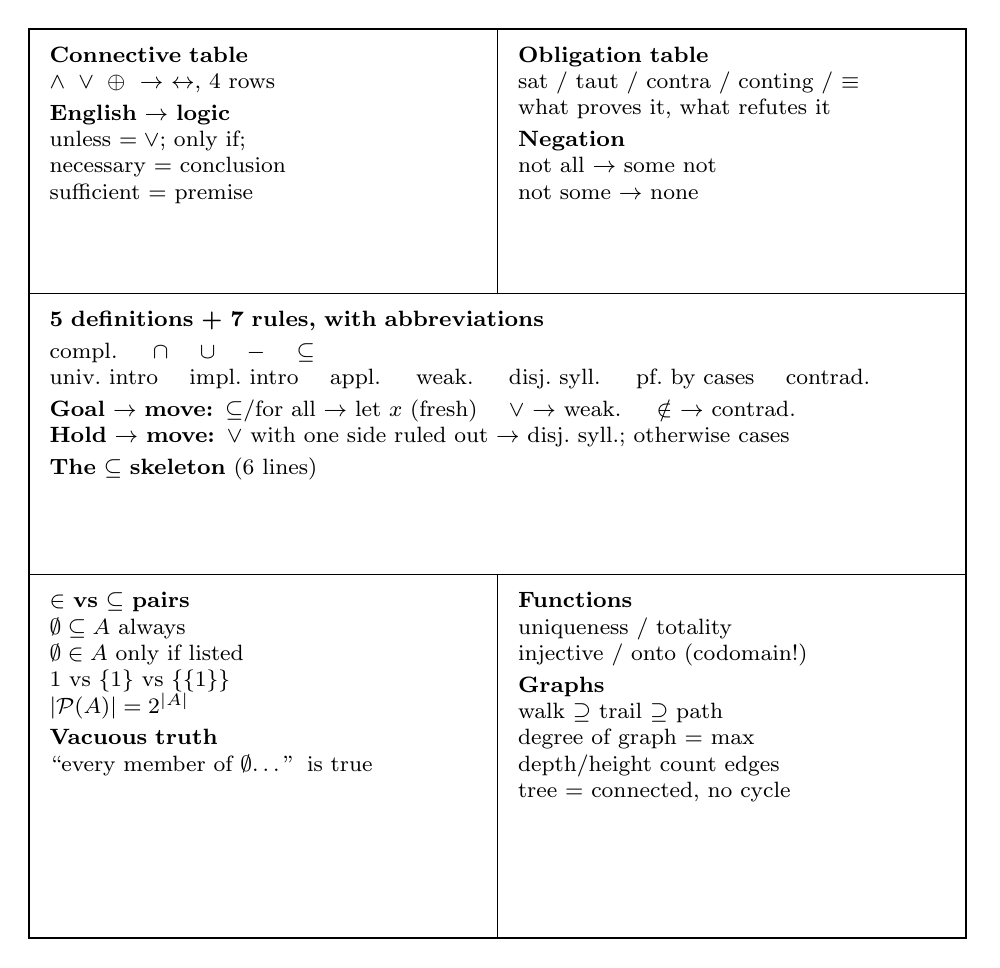
\begin{tikzpicture}[x=1.4cm,y=1.05cm,every node/.style={font=\footnotesize,align=left,anchor=north west}]
  \draw[line width=0.8pt] (0,0) rectangle (8.5,-11);
  \draw (0,-3.2) -- (8.5,-3.2);
  \draw (4.25,0) -- (4.25,-3.2);
  \draw (0,-6.6) -- (8.5,-6.6);
  \draw (4.25,-6.6) -- (4.25,-11);
  \node[text width=5.6cm] at (0.1,-0.1) {\textbf{Connective table}\\ $\land\ \lor\ \oplus\ \to\ \leftrightarrow$, 4 rows\\[2pt] \textbf{English $\to$ logic}\\ unless $=\lor$; only if;\\ necessary = conclusion\\ sufficient = premise};
  \node[text width=5.6cm] at (4.35,-0.1) {\textbf{Obligation table}\\ sat / taut / contra / conting / $\equiv$\\ what proves it, what refutes it\\[2pt] \textbf{Negation}\\ not all $\to$ some not\\ not some $\to$ none};
  \node[text width=11.6cm] at (0.1,-3.3) {\textbf{5 definitions + 7 rules, with abbreviations}\\[2pt]
    compl. \quad $\cap$ \quad $\cup$ \quad $-$ \quad $\subseteq$\\
    univ.\ intro \quad impl.\ intro \quad appl. \quad weak. \quad disj.\ syll. \quad pf.\ by cases \quad contrad.\\[2pt]
    \textbf{Goal $\to$ move:} $\subseteq$/for all $\to$ let $x$ (fresh) \quad $\lor$ $\to$ weak. \quad $\notin$ $\to$ contrad.\\
    \textbf{Hold $\to$ move:} $\lor$ with one side ruled out $\to$ disj.\ syll.; otherwise cases\\[2pt]
    \textbf{The $\subseteq$ skeleton} (6 lines)};
  \node[text width=5.6cm] at (0.1,-6.7) {\textbf{$\in$ vs $\subseteq$ pairs}\\ $\emptyset\subseteq A$ always\\ $\emptyset\in A$ only if listed\\ $1$ vs $\{1\}$ vs $\{\{1\}\}$\\ $|\mathcal{P}(A)|=2^{|A|}$\\[2pt] \textbf{Vacuous truth}\\ ``every member of $\emptyset$\dots'' is true};
  \node[text width=5.6cm] at (4.35,-6.7) {\textbf{Functions}\\ uniqueness / totality\\ injective / onto (codomain!)\\[2pt] \textbf{Graphs}\\ walk $\supseteq$ trail $\supseteq$ path\\ degree of graph = max\\ depth/height count edges\\ tree = connected, no cycle};
\end{tikzpicture}
\caption{One side of the note sheet. Notice what's missing: no worked proofs. If you need a full proof on the sheet to write one, that's the signal to do more practice, not to write smaller.}
\end{figure}

Write it by hand even if printed is allowed. Making the sheet is studying; printing it isn't.

\subsection{During the test}
\begin{enumerate}
\item \textbf{Read every question once before starting.} Do the compute-something questions first. They're fast and they calm you down.
\item \textbf{For a true/false claim, decide what kind of claim it is before deciding the answer.} ``For all'' claims need a general argument to prove but only one counterexample to refute. ``There exists'' claims are the other way around.
\item \textbf{For a proof, write the claim, then the first and last lines.} The first line is set by the goal's shape, and the last line is the conclusion you're aiming at. Fill in the middle afterwards. That alone is often worth partial credit.
\item \textbf{When stuck,} check three things in order. Am I using the right rule for the shape of the goal? Did I miscopy the claim, or make an earlier mistake? Is the claim actually false? If it might be false, try to make the premise true and the conclusion false with tiny sets.
\item \textbf{Don't bluff.} An honest, unfinished proof with no errors gets more credit than a ``complete'' one with a wrong step. Write ``I'd finish by showing \dots'' and move on.
\end{enumerate}

\subsection{The last 48 hours}
\begin{table}[H]\centering\small
\begin{tabularx}{\linewidth}{@{}p{2.6cm}L@{}}
\toprule
\textbf{When} & \textbf{What}\\
\midrule
Two days out & Practice sets from Chapters 2 and 3, cold and timed. Mark everything you missed.\\
Review session & Bring the missed list. Ask the scope questions: are functions and graphs on it? Is the sheet two-sided?\\
Night before & Write the note sheet. Redo only the problems you missed. No new material after that.\\
Morning of & One easy proof, one truth table, then stop. Eat something.\\
\bottomrule
\end{tabularx}
\end{table}

\vfill
\begin{center}\small
Found a mistake? Open an issue or a pull request on the repo. Corrections are welcome.
\end{center}


\end{document}
